\documentclass{ctuthesis}
\usepackage[table]{xcolor}
\usepackage{tabularx}
\usepackage{pifont}
\usepackage{fontawesome5}
\usepackage{algorithm}
\usepackage[noend]{algpseudocode}
\usepackage{listings}
\usepackage{caption, subcaption}
\newcommand{\algorithmautorefname}{Algorithm}

\ctusetup{
    xdoctype = B,
    xfaculty = F3,
    mainlanguage = english,
    titlelanguage = english,
    title-english = {Web application for managing group expenses},
    title-czech = {Webová aplikace pro správu a rozdělování výdajů ve skupině},
    department-english = {Department of Computer Science},
    author = {Stanislav Sadílek},
    supervisor = {Ing. Martin Ledvinka, Ph.D.},
    fieldofstudy-english = {Software Engineering and Technology},
    month = 5,
    year = 2026,
    keywords-czech = {skupinové výdaje, zjednodušení dluhů, správa výdajů, webová aplikace, Java, Spring Boot, React, REST, PostgreSQL},
    keywords-english = {group expenses, debt simplification, expense management, web application, Java, Spring Boot, React, REST, PostgreSQL}
}
    
\ctuprocess

\begin{thanks}
    I would like to thank my supervisor, Ing. Martin Ledvinka, Ph.D., for his expert guidance, valuable insights, and the time dedicated to our consultations. I truly appreciated his consistently supportive approach throughout the process. I would also like to thank my family and my girlfriend for their unwavering support.
\end{thanks}

\begin{declaration}
    I hereby declare that I have authored this bachelor's thesis independently and used only the sources listed at the end of the work, in accordance with the Methodological guideline on Adherence to Ethical Principles in Preparation of Graduation Theses.
    
\bigskip

    In Prague, 18th May 2026
\end{declaration}

\begin{abstract-english}
    Managing shared group expenses manually is a time-consuming and error-prone process. This thesis addresses these problems by developing SplitHappens, a web application that automates cost distribution and expense tracking.

    The thesis includes an analysis of user needs and current market alternatives to establish a foundation for a more effective, feature-rich solution. The resulting application provides a responsive interface and an optimized algorithm designed to settle debts with a minimal number of transactions. Evaluation through user testing confirmed that the application successfully simplifies shared expense tracking.
\end{abstract-english}
    
\begin{abstract-czech}
    Manuální správa výdajů ve skupině je časově náročný proces náchylný k chybám. Tato práce adresuje tyto problémy vývojem webové aplikace SplitHappens, která automatizuje rozdělování nákladů a sledování výdajů.

    Práce zahrnuje analýzu potřeb uživatelů a současných alternativ na trhu, aby vytvořila základ pro efektivní a funkční řešení. Výsledná aplikace poskytuje responzivní rozhraní a optimalizovaný algoritmus navržený k urovnání dluhů s minimálním počtem plateb. Hodnocení prostřednictvím uživatelského testování potvrdilo, že aplikace úspěšně zjednodušuje sledování společných výdajů.
\end{abstract-czech}

\begin{document}

\maketitle

\chapter{Introduction}
In groups of people, whether they are friends, family, or colleagues, situations often arise in which it is necessary to manage and divide group expenses; for example when shopping together, sharing accommodation, or traveling. Members of the group take turns covering various costs, after which the debts should be settled. However, handling this process manually is time-consuming and demanding and, more importantly, it is prone to inaccuracies and errors.

By leveraging modern technologies, this process can be simplified through a web application that automatically distributes expenses and provides each member with an overview of their balance.

\section{Objective}
The objective of this thesis is to design and implement a web application that not only clearly collects these group expenses but also minimizes the number of payments needed to fully settle all debts within the group. The design and functionality of the application are based on thorough research of already existing applications.  

\chapter{Analysis}
This chapter focuses on defining the scope of the project and its functionalities. First, user stories are described and divided into epics. The user stories are then further broken down into functional requirements, which are also assigned a priority based on their importance. 

Finally, a research of existing solutions was conducted, focusing on the most popular expense-sharing applications on the market. The research covered their advantages and disadvantages, as well as the availability of important features listed in functional requirements.

\section{User roles}
In the system, user roles determine the scope of accessible functionalities. This structure ensures both security and clarity of responsibilities. The application defines the following user roles:
\begin{itemize}
    \item \textbf{Guest} - has limited access, restricted to registration and signing in
    \item \textbf{User} - represents registered and logged in individual with full access to standard features, like group management or balance tracking
    \item \textbf{Admin} - a privileged user responsible for maintaining the system
\end{itemize}

\section{User Stories}
In software development, a user story describes a specific functionality of a software system using natural language~\cite{US1}. Written from the user's point of view, user stories put the user at the center of the development process and clearly outline the value the feature provides to the end user~\cite{US2, US3}. User stories follow a simple structure: As a <who>, I want <what> so that I <why>~\cite{US4}. This format provides developers with essential context while remaining understandable to everyone by using non-technical language~\cite{US3}.

For better organization, user stories were grouped into epics, which are used to create a hierarchy in the development process~\cite{Epic}. There are five epics:

\begin{itemize}
    \item User management
    \item Group management
    \item Expense management
    \item Payments and settlement
    \item Statistics and notifications
\end{itemize}


\subsection{Epic 1 - User management}
This epic covers basic user account operations, such as registration, login, and account maintenance. Guests can create new accounts or sign in, while administrators can manage user data. Authenticated users can also add friends.

\subsubsection{US01 - Registration}
As a Guest, I want to be able to create an account so I can start using the application.

\subsubsection{US02 - Login}
As a Guest, I want to be able to log in to my account using my credentials.

\subsubsection{US03 - Remove an account}
As an Admin, I want to view, edit, or delete accounts so that I can ensure system security and data integrity.

\subsubsection{US04 - Edit account information}
As a User, I want to edit my personal information so that my account details remain accurate and up to date.

\subsubsection{US05 - Add a friend}
As a User, I want to be able to add friends so that I can record non-group expenses and simplify adding people to new groups.


\subsection{Epic 2 - Group management}
Groups represent the core context for shared expenses. The second epic defines how users manage them within the application. Users can create groups, add members with existing accounts as well as placeholder members, and leave groups.
\subsubsection{US06 - Create a group}
As a User, I want to create a new group so that I can start tracking expenses.

\subsubsection{US07 - Invite registered users as members}
As a User, I want to be able to invite others to an existing group so that I can share expenses with them. New members can be added through a search.

\subsubsection{US08 - Leave a group}
As a User, I want to be able to leave a group when I no longer participate in its expenses so that I can keep my list of active groups clean and organized.

\subsection{Epic 3 - Expense management}
This epic outlines how users organize and record shared expenses within groups. Each expense can involve one or more payers and a selected set of participants. Users can categorize, filter and edit expenses to maintain accurate and well-organized data.

\subsubsection{US09 - Add an expense}
As a User, I want to add a new expense to a group so it can be shared among members. The payment can have one or more payers and any subset of members as participants, with the amount split between them by fixed amounts, percentages, or equal shares.

\subsubsection{US10 - Categorizing expenses}
As a User, I want to assign categories to expenses so that I can group payments with a similar purpose. 

\subsubsection{US11 - Filter and search expenses}
As a User, I want to search and filter through expenses by category or date so that I can quickly find specific transactions. 

\subsubsection{US12 - Edit or delete an expense}
As a User, I want to be able to edit or delete an expense in case I made a mistake.

\subsection{Epic 4 - Payments and settlement}
The fourth epic defines how debts resulting from payments are settled. Users are able to see their current balance at all times. The settlement process is simplified by automated calculations and the option to generate a QR code for quicker payments.

\subsubsection{US13 - View personal balance}
As a User, I want to see my personal balance across all groups I am part of, as well as my balance in every individual group by itself, so I have a clear overview of how much I owe or am owed.

\subsubsection{US14 - Simplify debts}
As a User, I want the system to simplify the debts between members so that the number of payments needed for settlement is minimal.

\subsubsection{US15 - Record a payment}
As a User, I want to record a payment to another user so that I can settle my debts.

\subsubsection{US16 - Generate a QR code for payment}
As a User, I want to be able to generate a QR code with payment information so that I settle debts quickly, whether I am sending money or receiving it from other users.

\subsection{Epic 5 - Statistics and notifications}
The last epic provides users with additional utilities, such as analytical insights and notifications related to their financial balance.
\subsubsection{US17 - Statistics and analytics}
As a User, I want a statistics dashboard so that I can analyze my spending across groups or categories. 

\subsubsection{US18 - Reminder notifications}
As a User, I want to send a notification to the users who owe me so that I can remind them to settle their debts.


\section{Functional Requirements}
Functional requirements are used to describe the features and functions of the system~\cite{FR1}. Unlike the user stories defined in the previous section, they are told from the system's point of view. Functional requirements are based directly on user stories. They are useful not only for defining the scope of the project in more detail, but also to help developers communicate with stakeholders~\cite{FR2}.

It is useful to prioritize functional requirements, as it highlights the crucial functionality of the system~\cite{FR2}. For this application, each requirement is assigned a priority value ranging from 1 (lowest) to 10 (highest). Based on these scores, the requirements are categorized into three priority levels. A complete list of prioritized functional requirements can be found in~\autoref{table:frq}.

\begin{itemize}
    \item \textbf{Core requirements} (8-10) represent essential functionality without which the system cannot meet its primary purpose.
    \item \textbf{Important requirements} (5-7) add significant value and improve the overall user experience. 
    \item \textbf{Enhancement requirements} (1-4) focus on optional, nice-to-have features.
\end{itemize}

\begin{table}[ht!]
\centering
\begin{tabularx}{\textwidth}{|X|p{2.7cm}|l|}
\hline
\textbf{Requirement} & \textbf{Priority group} & \textbf{Priority} \\ \hline

FRQ01 - Registration & Core & 10 \\ \hline
FRQ02 - Authentication and authorization & Core & 10 \\ \hline
FRQ08 - Group viewing & Core & 10 \\ \hline
FRQ11 - Group detail & Core & 10 \\ \hline
FRQ14 - Adding an expense & Core & 10 \\ \hline
FRQ15 - Expense detail & Core & 10 \\ \hline
FRQ22 - Personal balance & Core & 10 \\ \hline
FRQ23 - Debt simplification algorithm & Core & 10 \\ \hline
FRQ24 - Recording a payment & Core & 10 \\ \hline
FRQ03 - User management & Core & 9 \\ \hline
FRQ04 - Edit a profile & Core & 9 \\ \hline
FRQ09 - Group management & Core & 9 \\ \hline
FRQ12 - Add members to a group & Core & 9 \\ \hline
FRQ21 - Expense editing and deletion & Core & 9 \\ \hline
FRQ05 - User listing and search & Core & 8 \\ \hline
FRQ13 - Leaving a group & Core & 8 \\ \hline
FRQ20 - Expense filtering and search & Core & 8 \\ \hline

FRQ18 - Expense categories & Important & 7 \\ \hline
FRQ26 - Generating QR codes & Important & 7 \\ \hline
FRQ06 - Adding a friend & Important & 6 \\ \hline
FRQ07 - Friend request handling & Important & 6 \\ \hline
FRQ27 - Group statistics & Important & 6 \\ \hline
FRQ16 - Non-group expenses & Important & 5 \\ \hline

FRQ29 - Notifications & Enhancement & 4 \\ \hline
FRQ19 - Custom categories & Enhancement & 3 \\ \hline
FRQ25 - Multi-group friend debt settling & Enhancement & 3 \\ \hline
FRQ30 - Sending a reminder & Enhancement & 3 \\ \hline
FRQ17 - Multi currency support & Enhancement & 2 \\ \hline
FRQ28 - User statistics & Enhancement & 2 \\ \hline
FRQ10 - Group permissions & Enhancement & 1 \\ \hline

\end{tabularx}
\caption{Functional requirements sorted by priority}
\label{table:frq}
\end{table}



\subsubsection{FRQ01 - Registration (Core)}
The system will allow new users to create an account by filling out a registration form with their personal data and credentials.

\subsubsection{FRQ02 - Authentication and authorization (Core)}
The system must provide secure login functionality for all users using role based access control to ensure appropriate access permissions.

\subsubsection{FRQ03 - User management (Core)}
The system shall give administrators the ability to edit or delete other accounts.

\subsubsection{FRQ04 - Edit a profile (Core)}
The system offers the option to edit a profile with all personal information.

\subsubsection{FRQ05 - User listing and search (Core)}
The system allows users to list and search through other users.

\subsubsection{FRQ06 - Adding a friend (Important)}
The system will allow users to add other users as friends.

\subsubsection{FRQ07 - Friend request handling (Important)}
The system offers the option to a user who has received a friend request with the choices to accept or reject.

\subsubsection{FRQ08 - Group Viewing (Core)}
The system provides users with a list of all groups they are part of. Groups that are settled and inactive for a long time are pushed to the bottom of the list.

\subsubsection{FRQ09 - Group management (Core)}
The system allows users to create or edit groups. Administrators can also delete them, but the group must be settled before it can be deleted. 

\subsubsection{FRQ10 - Group permissions (Enhancement)}
The system shall let users to choose between two permission types when creating a group. In soft mode (default), everyone can edit all expenses and add or remove other members. On the other hand, if the group is set to strict mode, members can only edit their own expenses, and only the owner (or members chosen by the owner) can add or remove other members.

\subsubsection{FRQ11 - Group detail (Core)}
The system provides users with a group overview page, where they can see their balance, as well as recent expenses and payments.

\subsubsection{FRQ12 - Add members to a group (Core)}
The system will allow users to add new members to an existing group. Adding a member does not affect existing expenses or balances.

\subsubsection{FRQ13 - Leaving a group (Core)}
The system gives users the option to leave a group. A user must be settled in that group to be able to leave it. 

\subsubsection{\label{frq:14}FRQ14 - Adding an expense (Core)} 
The system allows users to add an expense to a group. They can set any number of members of the group as the payers (members who paid the expense) and as participants (members among whom the expense is split). The amount can be divided between both payers and participants by fixed amounts, percentages, or equal shares.

\subsubsection{FRQ15 - Expense detail (Core)}
The system grants access to expense details, where users can see all information about the specific expense, including the participants, the payers, and their respective shares.

\subsubsection{\label{frq:16}FRQ16 - Non-group expenses (Important)}
The system gives users the option to add a non-group expense. This type of expense can only be recorded between two users (friends) and cannot be shared or split among multiple participants.

\subsubsection{FRQ17 - Multi currency support (Enhancement)}
The system provides multi currency support, which means that users can add expenses in various currencies in one group. The system automatically calculates the currency exchange based on the current rate at the time the expense is created. The resulting balance is shown in the default currency of the group, which is set during group creation.

\subsubsection{FRQ18 - Expense categories (Important)}
The system offers to divide the expenses into categories. This can be done either when adding an expense or later during editing.

\subsubsection{FRQ19 - Custom categories (Enhancement)}
The system supports creating custom categories to make categorization more flexible. Custom categories are kept separately for each group.

\subsubsection{FRQ20 - Expense filtering and search (Core)}
The system will allow users to search for expenses and filter them by category. Expenses are also automatically grouped into expandable sections by month.

\subsubsection{FRQ21 - Expense editing and deletion (Core)}
The system allows users to edit or delete existing expenses and payments based on group permission settings. Users can edit or delete all expenses in soft mode, whereas in strict mode, they can only modify and remove their own expenses.

\subsubsection{FRQ22 - Personal balance (Core)}
The system provides users with a clear overview of their balance. It is shown both in the group list, which summarizes the balance across all groups, and within a group overview.

\subsubsection{FRQ23 - Debt simplification algorithm (Core)}
The system implements an algorithm for simplifying debts within a group, so the least number of payments must be made to settle the entire group's debts. This optimization may produce outcomes that look counterintuitive. For example, one user may owe money to another who did not directly pay for them.

\subsubsection{FRQ24 - Recording a payment (Core)}
The system allows users to record a payment to settle their debts.

\subsubsection{FRQ25 - Multi-group friend debt settling (Enhancement)}
The system offers the option to settle a debt with another user via the friends list.

\subsubsection{FRQ26 - Generating QR codes (Important)}
The system provides an interface for generating a QR code with the necessary banking information to enable quick and simple payment. It is worth noting that a bank account is not required when creating an account, therefore this feature might not be available for all users.

\subsubsection{FRQ27 - Group statistics (Important)} 
The system provides users with group statistics that contain detailed information about expenses based on categories, spending, or payments.

\subsubsection{FRQ28 - User statistics (Enhancement)}
The system provides users with an overview of their personal spending in all groups. This view includes totals or category breakdowns.

\subsubsection{\label{frq:29}FRQ29 - Notifications (Enhancement)}
The system supports sending notifications to users when important events occur, such as when a user was added to a group, was involved in a new expense, or received a friend request.

\subsubsection{\label{frq:30}FRQ30 - Sending a reminder (Enhancement)}
The system offers users the ability to send reminders to other members about outstanding balances. A reminder notifies the recipient about unpaid debts, including relevant context such as group or amount owed.

\section{Existing solutions}
There are various applications on the market that focus on group expense management, differing in both functionality and user interface. This chapter provides an overview of some of the most popular ones. These applications were selected based on the number of downloads on Google Play, with each of them having more than one million downloads. It is worth noting that these are mobile applications — some of which also offer a web interface. At the end of this chapter, a comparison table summarizing their key features is included. The following four applications were chosen:
\begin{itemize}
    \item Splitwise
    \item Tricount
    \item Settle Up
    \item Splid
\end{itemize}

\subsection{Splitwise}
Splitwise is one of the most well-known expense-tracking apps worldwide, with over 10 million downloads~\cite{Split1, Split2}. Its popularity makes it an excellent choice when forming a new group, as many users already have the app installed, unlike some less popular alternatives. Splitwise offers a wide range of features, such as splitting an expense among multiple payers. You can also manage expenses in multiple currencies.

One of the biggest drawbacks of Splitwise is that its free version is lately becoming increasingly limited. The app has received significant criticism for limiting the number of added expenses, which is a reason why many users are looking for other options~\cite{Split3}. Additionally, Splitwise may feel too complex for users seeking basic functionality.

Splitwise does not offer any connection to payment systems. Although this might seem like a flaw, some users prefer to manage payments separately without being tied to specific payment platforms. Screenshots from the Splitwise mobile application are shown in~\autoref{fig:split}.
\subsubsection{Pros}
\begin{itemize}
    \item Wide range of functionalities
    \item Large user base
\end{itemize}

\subsubsection{Cons}
\begin{itemize}
    \item Aggressive free version limitations
    \item May feel heavyweight
\end{itemize}

\begin{figure}[h]
    \centering
    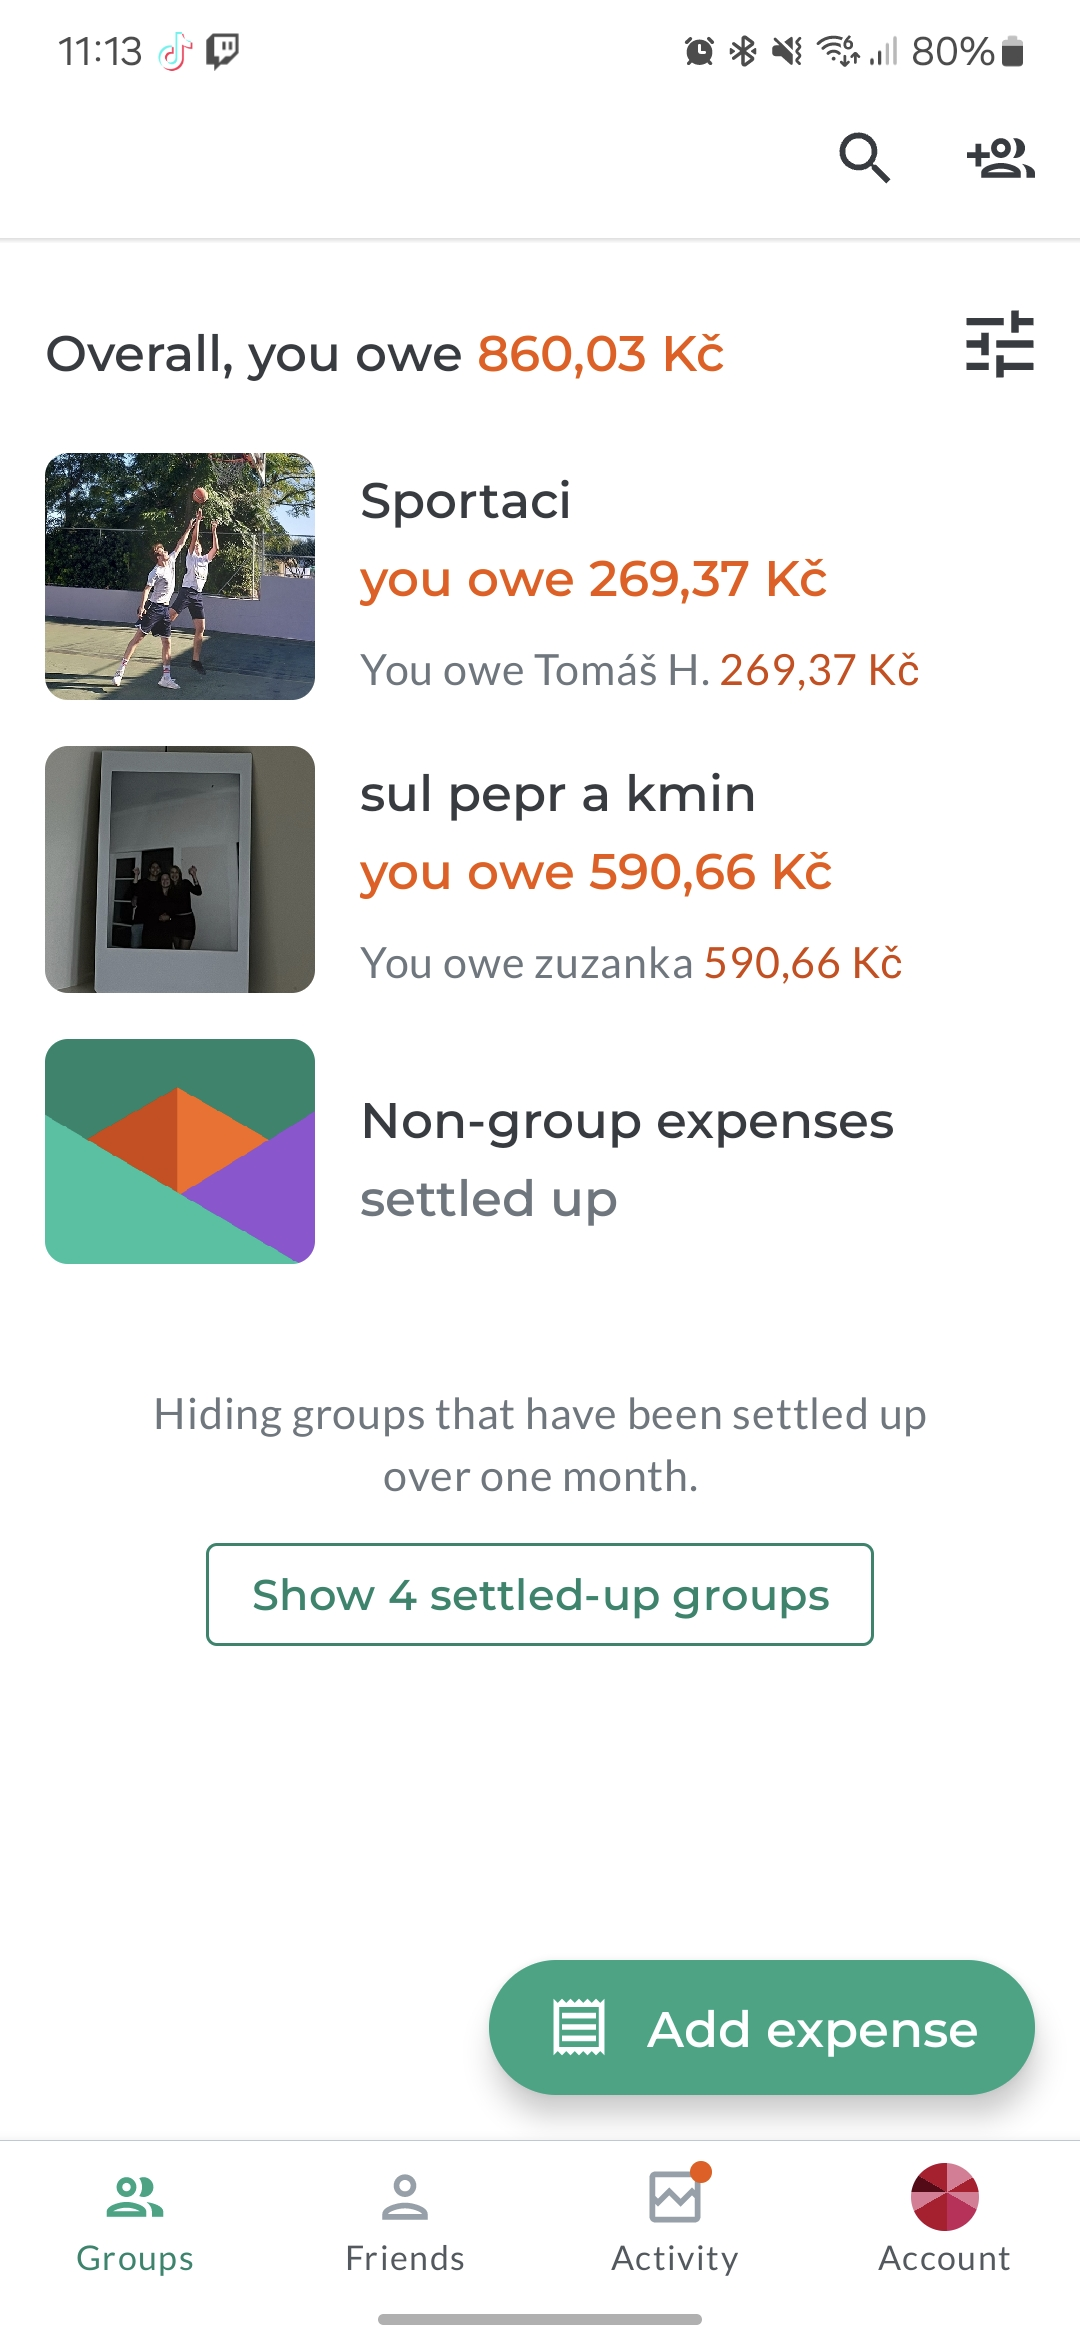
\includegraphics[scale=0.11]{images/existing/split1.jpg}
    \hspace{35pt}
    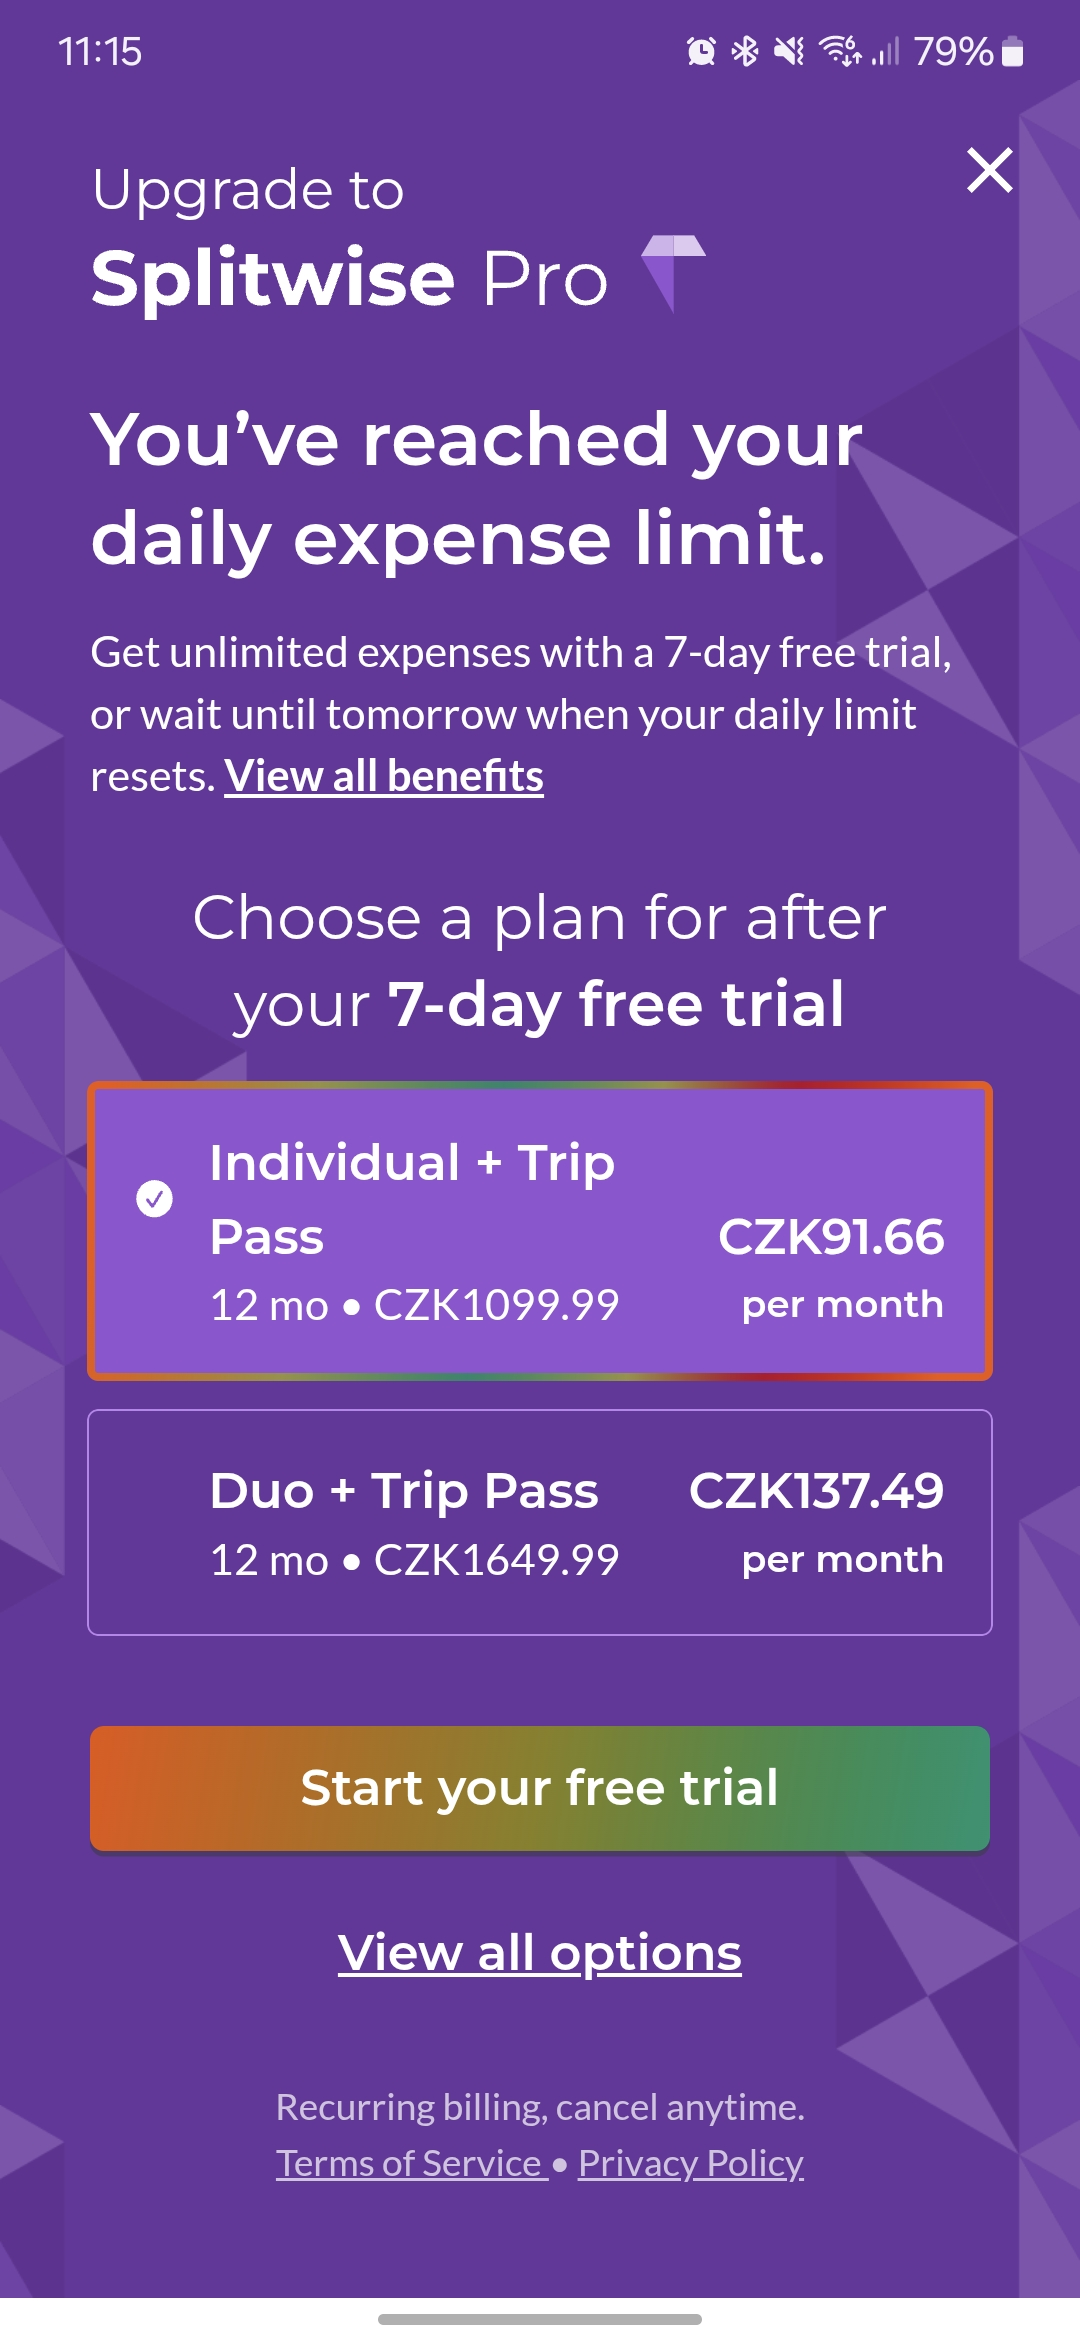
\includegraphics[scale=0.11]{images/existing/split2.jpg}
    \caption{Splitwise screenshots showcasing group list and hitting the daily expense limit. Source: Author}
    \label{fig:split}
\end{figure}

\subsection{Tricount}
Tricount is one of the biggest competitors to Splitwise. It takes a more lightweight approach to shared expense management. There is no required account registration, so users can get started immediately~\cite{Tri1}. Additionally, the app has recently moved away from a paid subscription, and all its features are available for free. It can even be used offline — expenses will be synced automatically when the user is back online. Tricount also supports adding expenses in multiple currencies within one group~\cite{Tri2}. To make switching platforms easier, the app offers the option to import existing data from Splitwise, attracting more users who are dissatisfied with Splitwise. 

However, Tricount also comes with notable downsides. Some more complex features, such as splitting a single expense between multiple payers, are not supported. Furthermore, Tricount does not have a web-based application and can only be used on mobile devices. These limitations make Tricount less suitable for users who need advanced control over their expenses in more complicated scenarios.

Tricount supports bank account connections for quick and simple payments. It also offers a virtual credit card that automatically records and splits expenses when used~\cite{Tri3}. \autoref{fig:tricount} showcases group details and payment addition process in the Tricount mobile application.

\subsubsection{Pros}
\begin{itemize}
    \item Unlimited free access
    \item Offline mode
    \item No registration needed
\end{itemize}

\subsubsection{Cons}
\begin{itemize}
    \item No web-application
    \item Lacks advanced expense splitting
\end{itemize}

\begin{figure}[h]
    \centering
    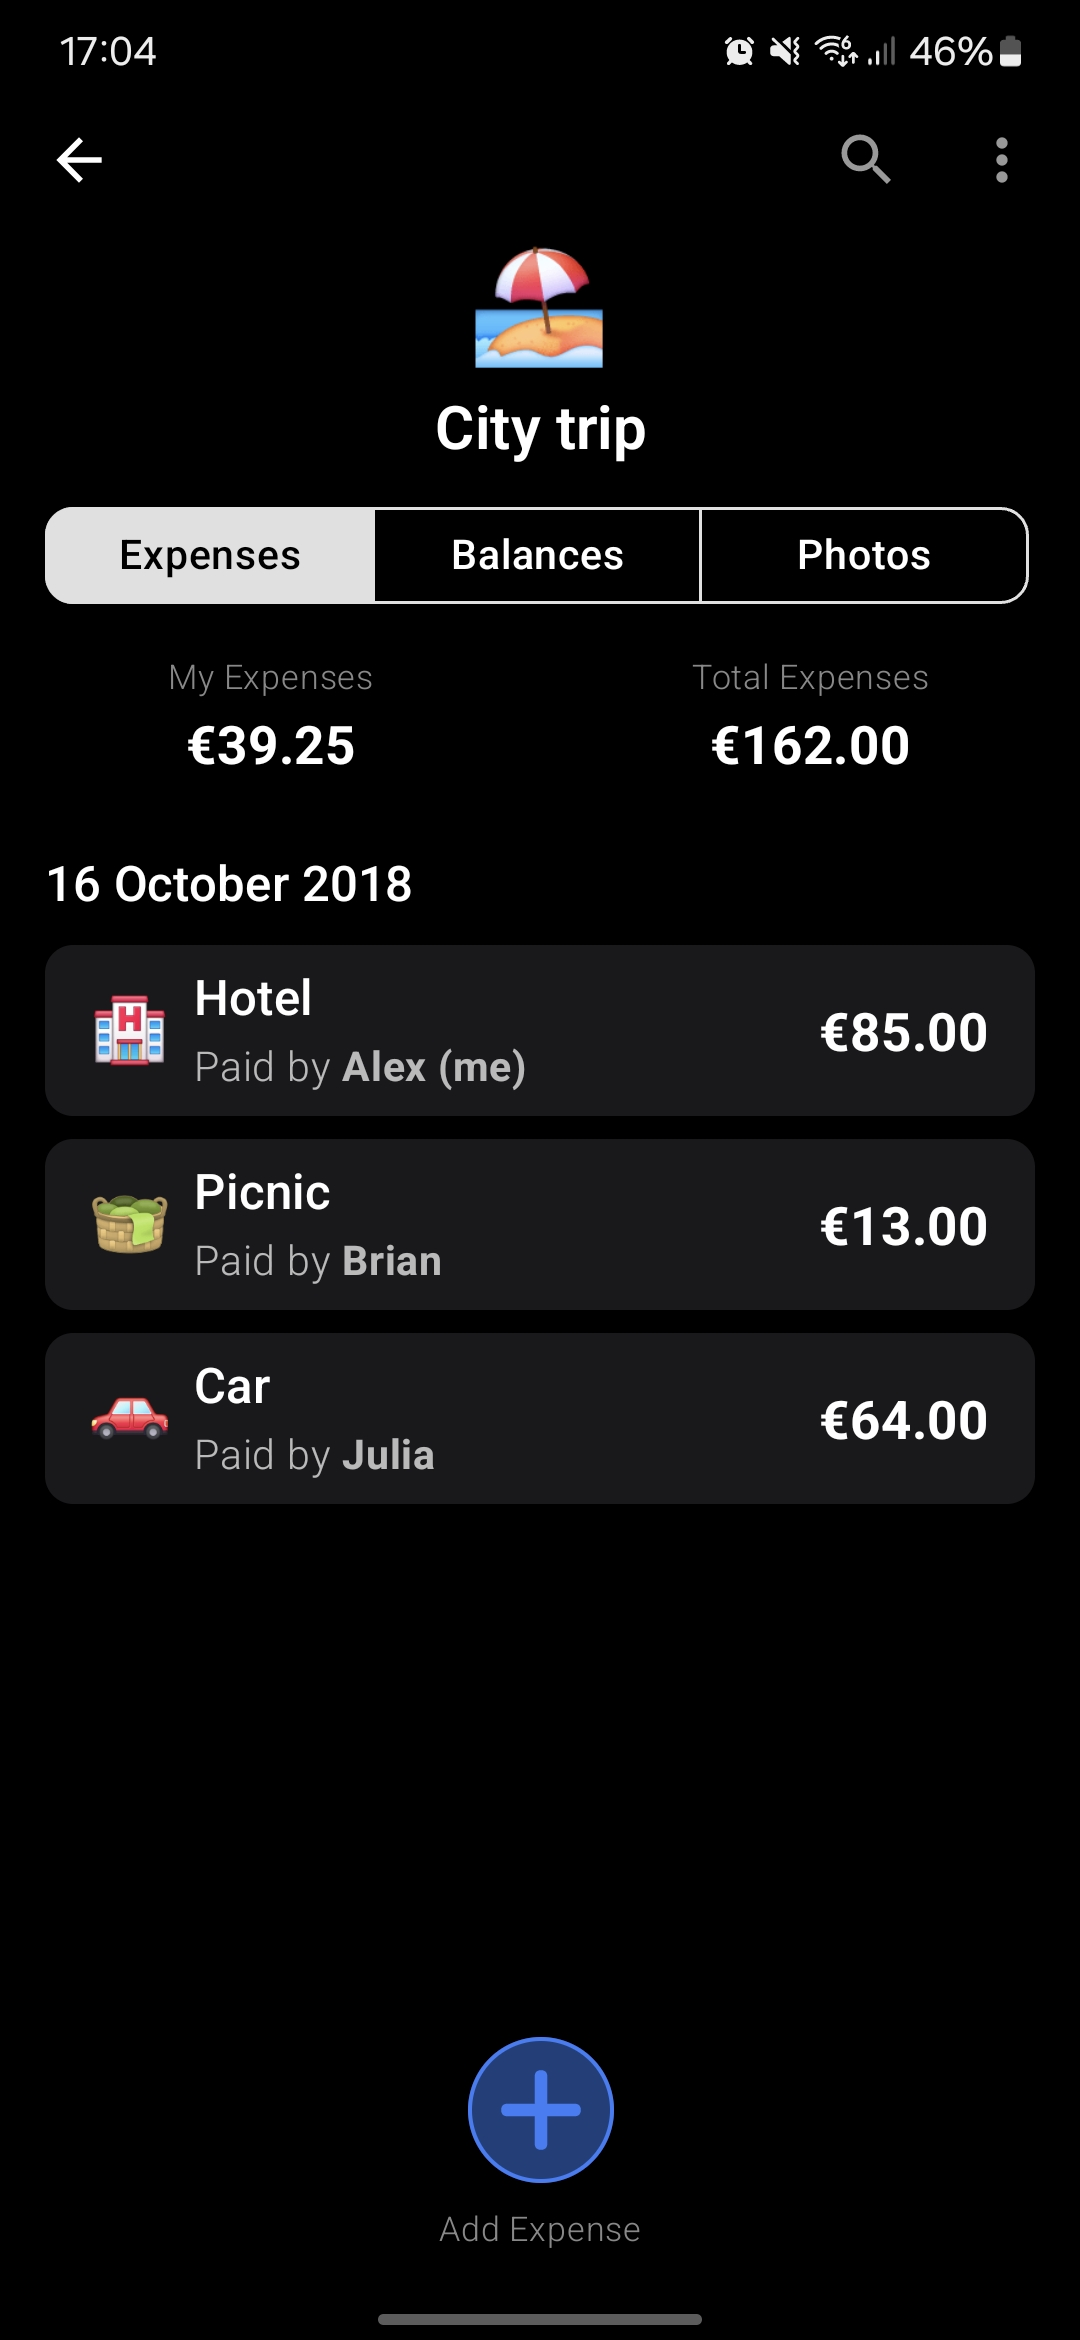
\includegraphics[scale=0.11]{images/existing/tricount1.jpg}
    \hspace{35pt}
    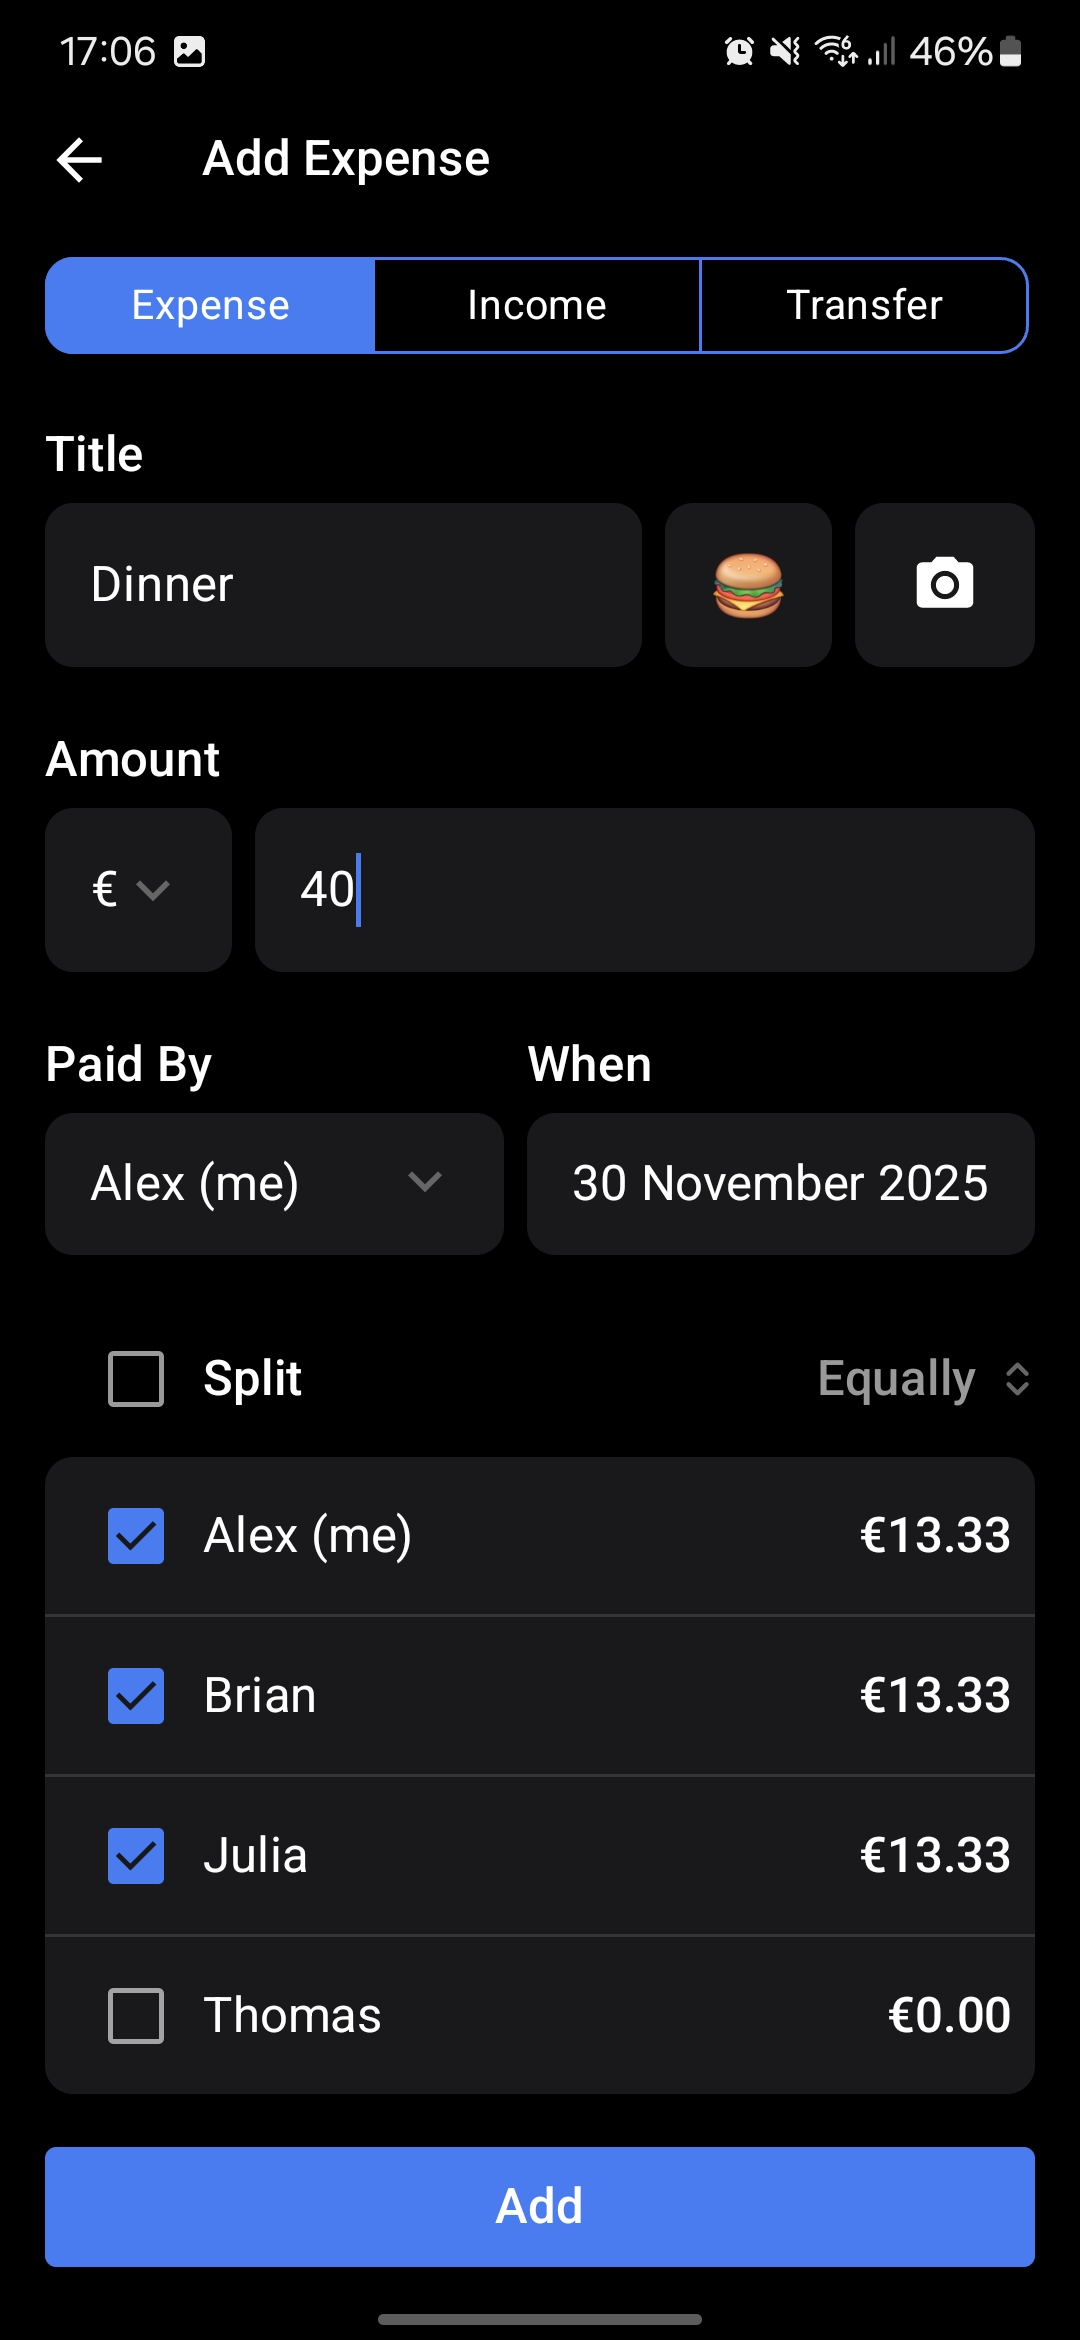
\includegraphics[scale=0.11]{images/existing/tricount2.jpg}
    \caption{Tricount screenshots of group detail and the interface for adding expenses. Source: Author}
    \label{fig:tricount}
\end{figure}

\subsection{Settle Up}
Another popular tool for managing expenses in groups is Settle Up. It offers a wide range of features, including group permissions, built-in currency conversion, and advanced expense splitting, allowing users to assign multiple payers to a single expense~\cite{SettleUp1}.

Nevertheless, many of its features are locked behind a paywall. Functionalities like categories, statistics, image upload (for example, for receipts) or reminders are available for premium users only. The subscription offers two plans: Individual, which applies to a single user with monthly or yearly billing, and Group, which applies to a group and provides a lifetime purchase option on top of weekly, monthly and yearly billing~\cite{SettleUp2}. Additionally, Settle Up does not support adding friends and non-group expenses.

Unlike Tricount, Settle Up does not provide direct bank account connections. Instead, the app includes the functionality to generate QR codes to settle debts. Screenshots from Settle Up can be seen in \autoref{fig:settleup}.

\subsubsection{Pros}
\begin{itemize}
    \item Advanced expense splitting
    \item Has a web application
\end{itemize}

\subsubsection{Cons}
\begin{itemize}
    \item Paywall for many features
    \item Requires registration
\end{itemize}

\begin{figure}[h]
    \centering
    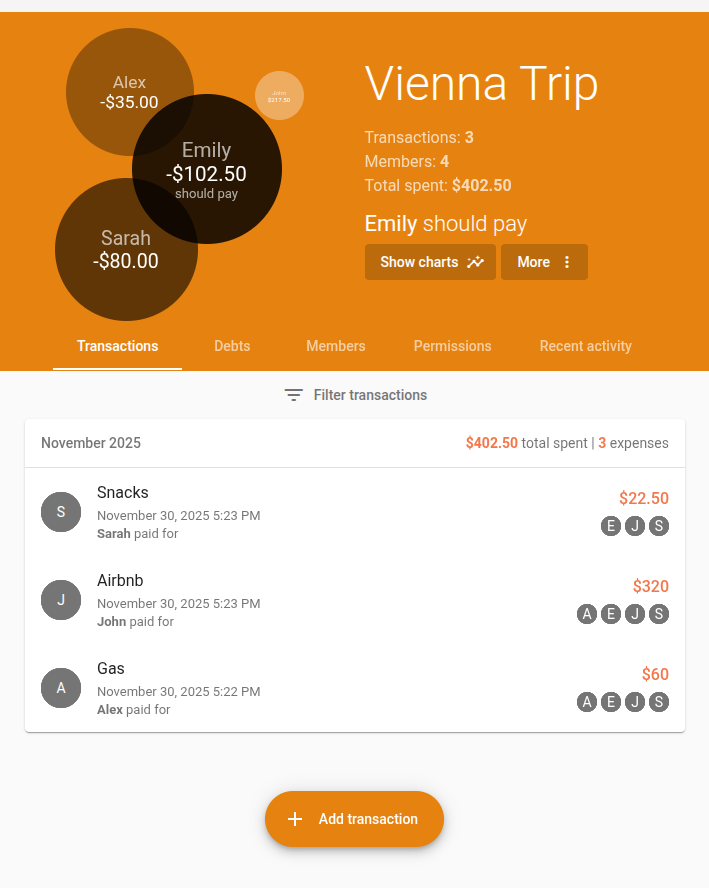
\includegraphics[scale=0.25]{images/existing/settleup1.png}
    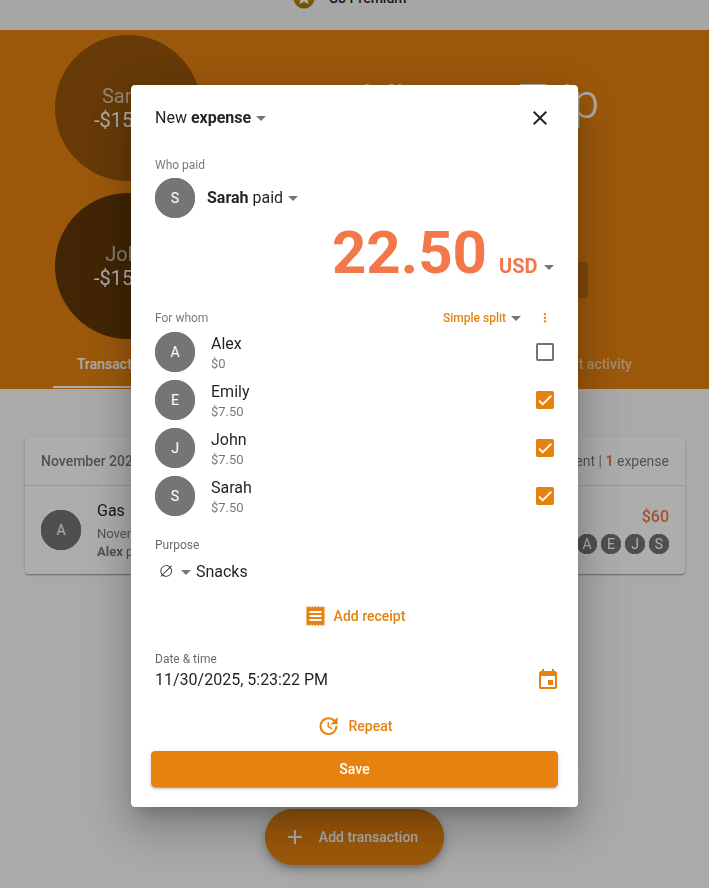
\includegraphics[scale=0.25]{images/existing/settleup2.png}
    \caption{Settle Up screenshots showcasing group detail and adding an expense. Source: Author}
    \label{fig:settleup}
\end{figure}

\subsection{Splid}
The last application covered in this analysis is Splid. Splid offers a clean and simple interface focused on the core purpose: tracking shared expenses. It does not require user registration, making it very easy to set up. Splid also supports data export to PDF and Excel, although Excel export is available in the premium version only.

However, Splid is not the best option for users looking for a desktop version, as it works only as a mobile app. Some features are also limited to the premium version, such as creating more than two groups, Excel export, or advanced statistics.

The app does not include any payment integration, so settling balances must be done outside the platform. \autoref{fig:splid} illustrates the user interface of Splid mobile app.

\subsubsection{Pros}
\begin{itemize}
    \item Offline mode
    \item Export to PDF
\end{itemize}

\subsubsection{Cons}
\begin{itemize}
    \item Fewer features
    \item Lower user base
\end{itemize}

\begin{figure}[h]
    \centering
    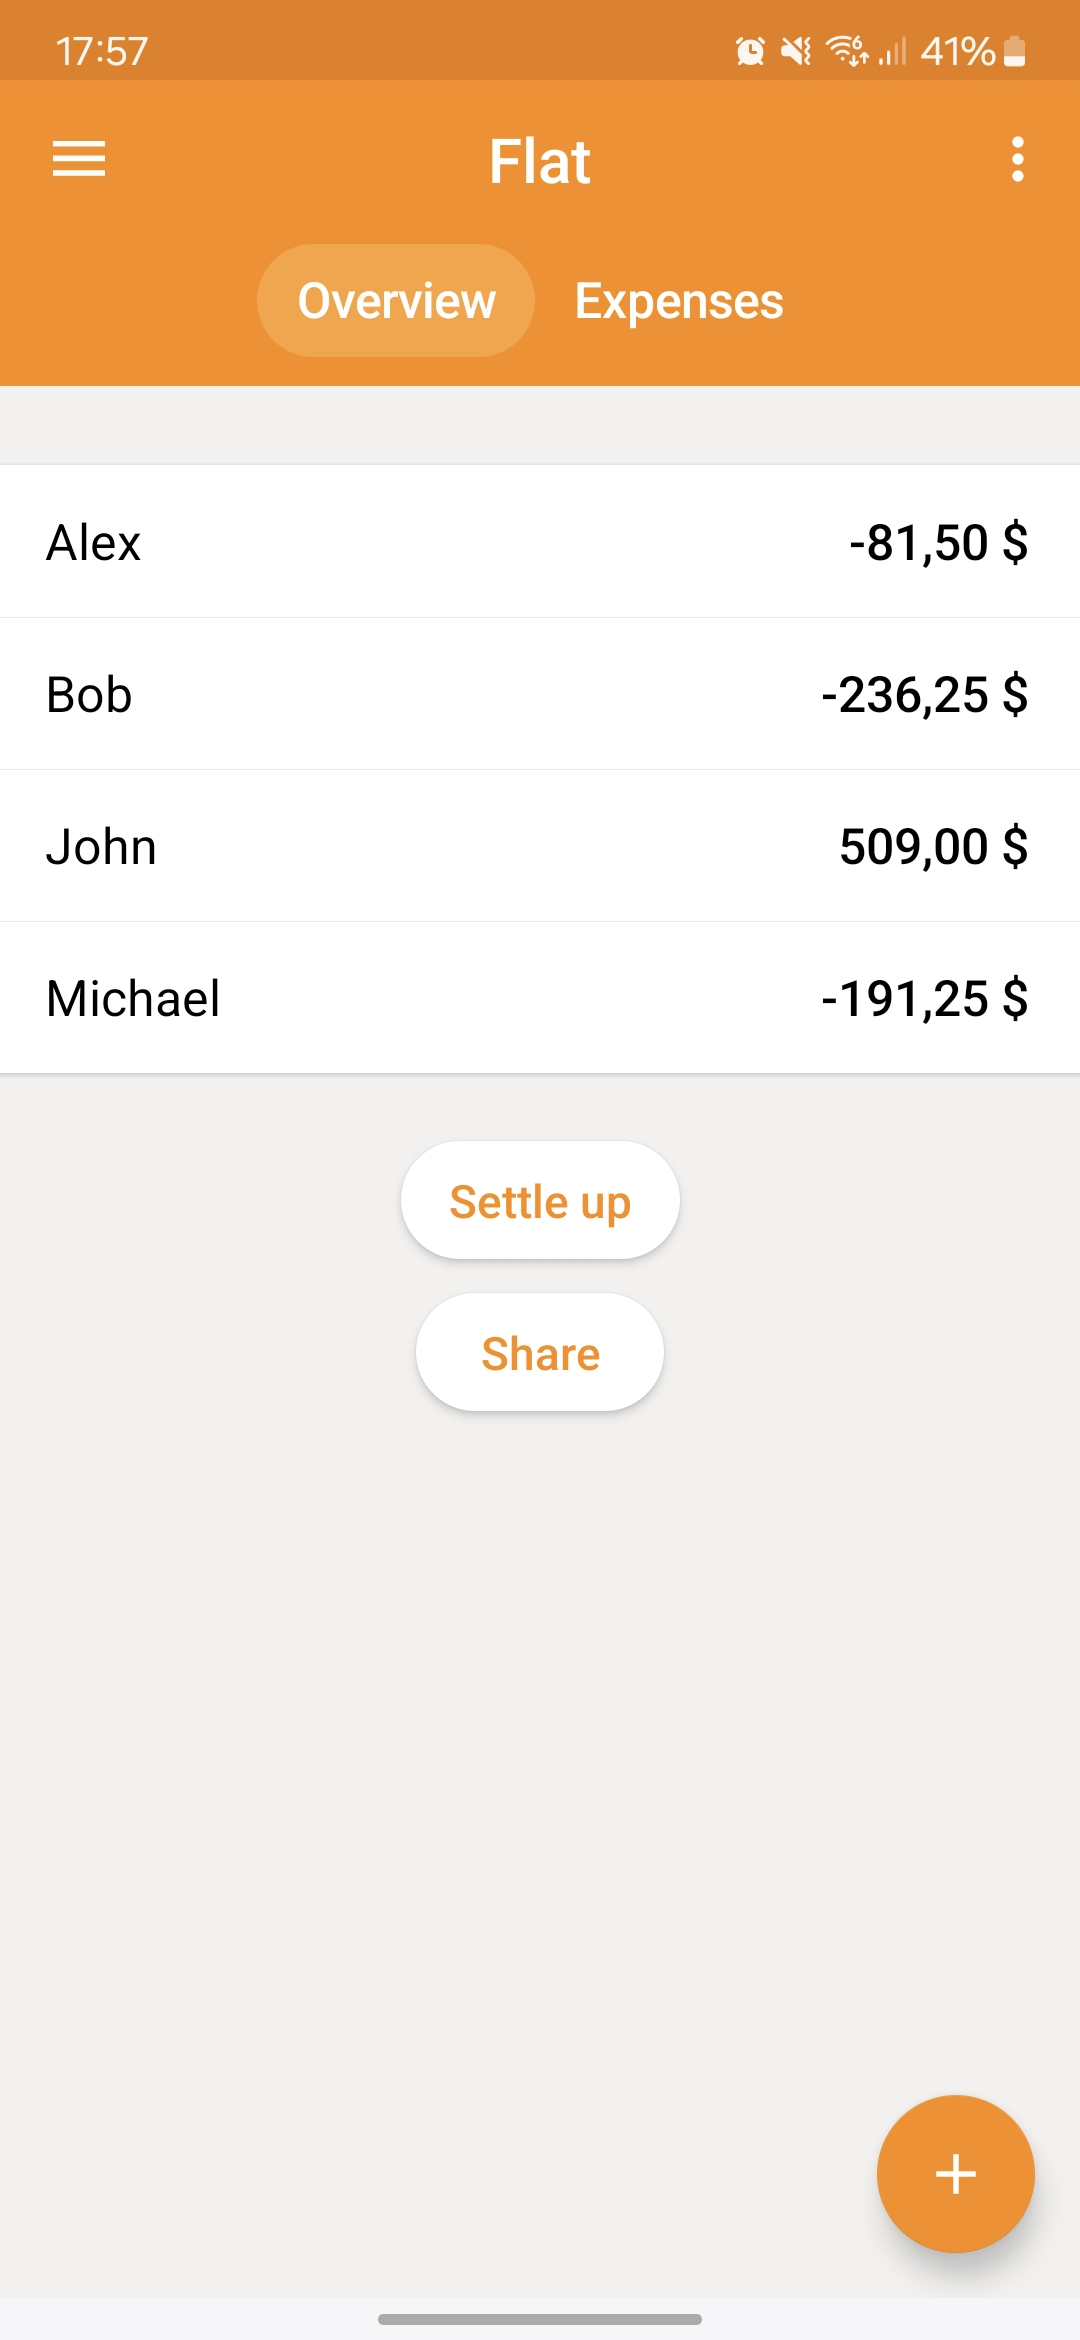
\includegraphics[scale=0.11]{images/existing/splid1.jpg}
    \hspace{35pt}
    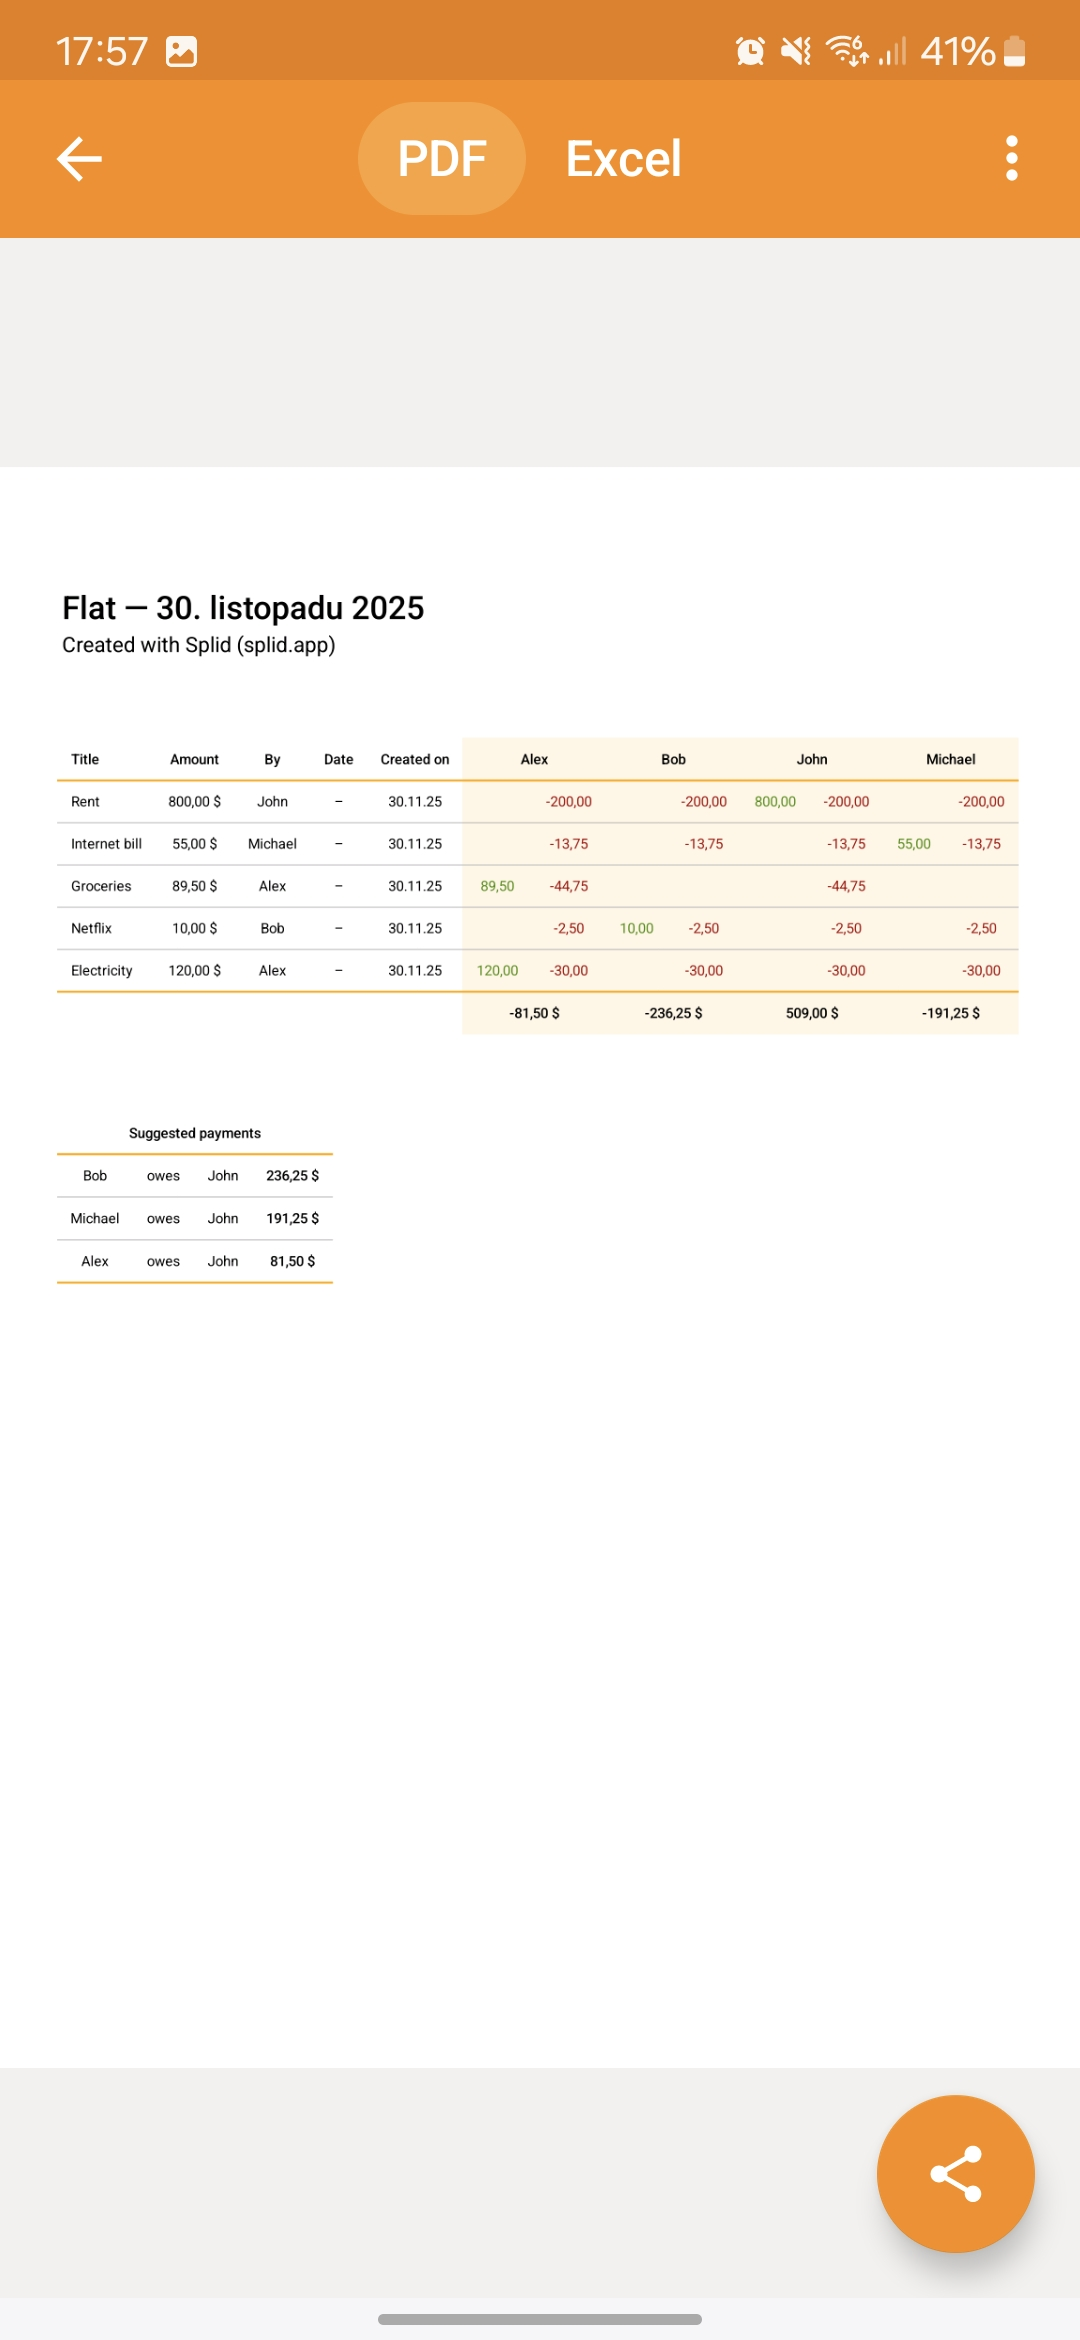
\includegraphics[scale=0.11]{images/existing/splid2.jpg}
    \caption{Splid screenshots featuring group detail and export to PDF. Source: Author}
    \label{fig:splid}
\end{figure}

\subsection{Summary}
To provide a clearer overview of the strengths and weaknesses of existing solutions, \autoref{table:features_apps} compares the key features of the selected applications. The comparison highlights their similarities and differences.
\begin{table}[ht!]
    \begin{tabularx}{\textwidth}{|l||>{\centering}X|>{\centering}X|>{\centering}X|>{\centering\arraybackslash}X|}
     \hline
     & \textbf{Splitwise}  & \textbf{Tricount} & \textbf{Settle up} & \textbf{Splid} \\  
     \hline
     Full free access      & \ding{55}   & \ding{51} & \ding{55}   & \ding{55} \\  
     \hline
     Advance expense splitting    & \ding{51}   & \ding{55} & \ding{51}   & \ding{51} \\ 
     \hline
     Expense categories    & \ding{51}   & \ding{55} & \textbf{\$} & \ding{55} \\  
     \hline
     Friends    & \ding{51}   & \ding{55} & \ding{55}   & \ding{55} \\ 
     \hline
     Statistics            & \textbf{\$} & \ding{51} & \textbf{\$} & \textbf{\$} \\
     \hline
     Non-group expenses    & \ding{51}   & \ding{55} & \ding{55}   & \ding{55} \\ 
     \hline
     Multi-currency        & \ding{51}   & \ding{51} & \ding{51}   & \ding{55} \\  
     \hline
     Usable without registration & \ding{55}   & \ding{51} & \ding{55}   & \ding{51} \\ 
     \hline
     Web access            & \ding{51}   & \ding{55} & \ding{51}   & \ding{55} \\  
     \hline
     Payment integration   & \ding{55}   & \ding{51} & \ding{51}   & \ding{55} \\  
     \hline
     Custom categories    & \ding{55}   & \ding{55} & \ding{55}   & \ding{51} \\ 
     \hline
     Group permissions    & \ding{55}   & \ding{55} & \ding{51}   & \ding{55} \\ 
    \hline
    \end{tabularx}
    \raggedright
    \footnotesize
    \textbf{Legend:} \ding{51} = Feature available, \ding{55} = Feature not available, \textbf{\$} = Paid feature.
    \caption{Features of existing applications}
    \label{table:features_apps}
\end{table}

\chapter{Design}
This chapter focuses on the next step of the development process, moving from analysis to design. Firstly, the choice of architecture will be covered, followed by a demonstration of the user interface prototype, showcasing the design of key parts of the application.

\section{Architecture style}
This section outlines the architecture of the system, which is designed as a web application based on the client-server model to prioritize cross-platform accessibility. The server-side logic follows a layered architecture for maintainability reasons. These choices are detailed in the following subsections with a further description of the system in the domain model and the component diagram.

\subsection{Platform}
Based on the market analysis in the last chapter, it was observed that the majority of existing solutions are native mobile applications. To differentiate the proposed solution and maximize accessibility, the decision was made to develop a web application. This allows users to access the system via any device with a web browser without the need for installation.

\subsection{Client-server model}
The client-server architecture is a fundamental approach that divides the functionality of a system between a client and a server~\cite{fundamentals}. This is an efficient way to separate different parts of a software application. The client part focuses on the user interface and presentation, while the server manages the core logic and data storage. Visualization of this architecture can be seen in \autoref{fig:clientserver}.

\begin{figure}[h]
    \centering
    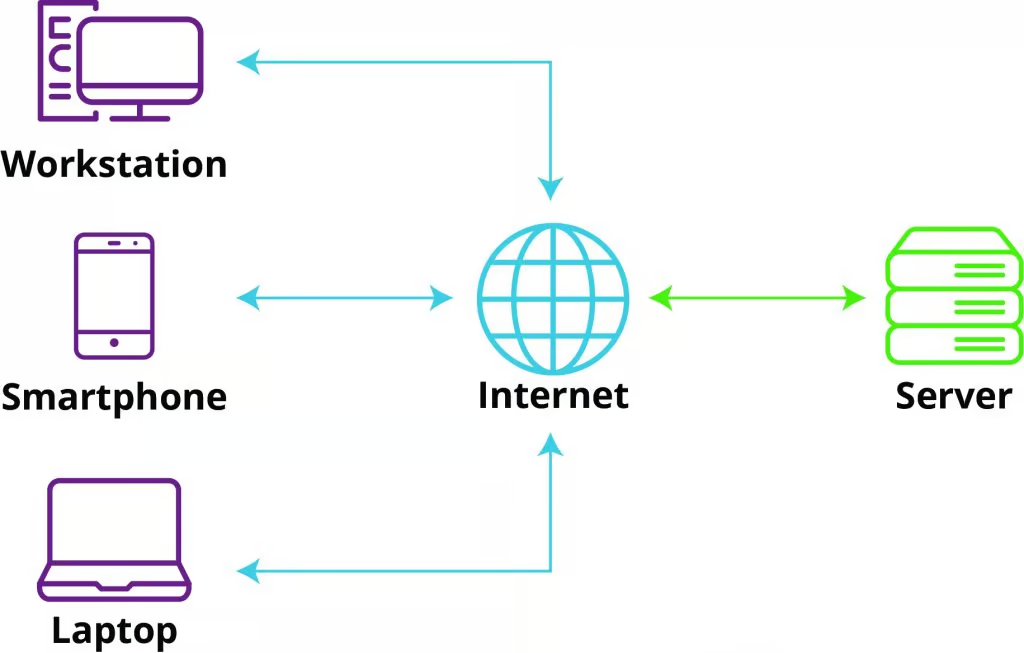
\includegraphics[width=0.7\linewidth]{images/architecture/client-server.png}
    \caption{Client-server architecture~\cite{clientserver}}
    \label{fig:clientserver}
\end{figure}

This centralized design simplifies system management by keeping all data in one place. However, the same centralization creates a single point of failure vulnerability (SPOF), meaning that a server crash can shut down the whole system~\cite{clientserver}.

The client-server architecture was chosen for this application mainly for its simplicity of design and maintenance that outweighs the problem of SPOF, which can be mitigated through replication.

\subsection{Layered architecture}
Layered architecture is one of the most used architecture styles in software development~\cite{fundamentals}. The components of the system are organized into horizontal layers, where each layer has a specific role. In a strict layered architecture, each layer should only interact with the layer directly below it~\cite{patterns}. This structure promotes the separation of concerns, which means that business rules remain independent of the user interface and the database. Layered architecture typically consists of three layers~\cite{patterns}.
\begin{itemize}
    \item \textbf{Presentation layer} handles the interaction between the client and the application.
    \item \textbf{Business logic layer} contains the business logic of the system and performs validations. 
    \item \textbf{Data source layer} handles the communication with the database to retrieve and store data.
\end{itemize}

For this application, the layered architecture was chosen because it provides a clear and maintainable structure.

\subsection{\label{domain-model}Domain model}
A domain model is a network of connected objects that represent specific entities and their attributes~\cite{patterns}. The diagram presented in~\autoref{fig:class} illustrates the UML class diagram for this application, defining core entities such as users, groups, and transactions, and the relationships between them. 

\begin{figure}[h]
    \centering
    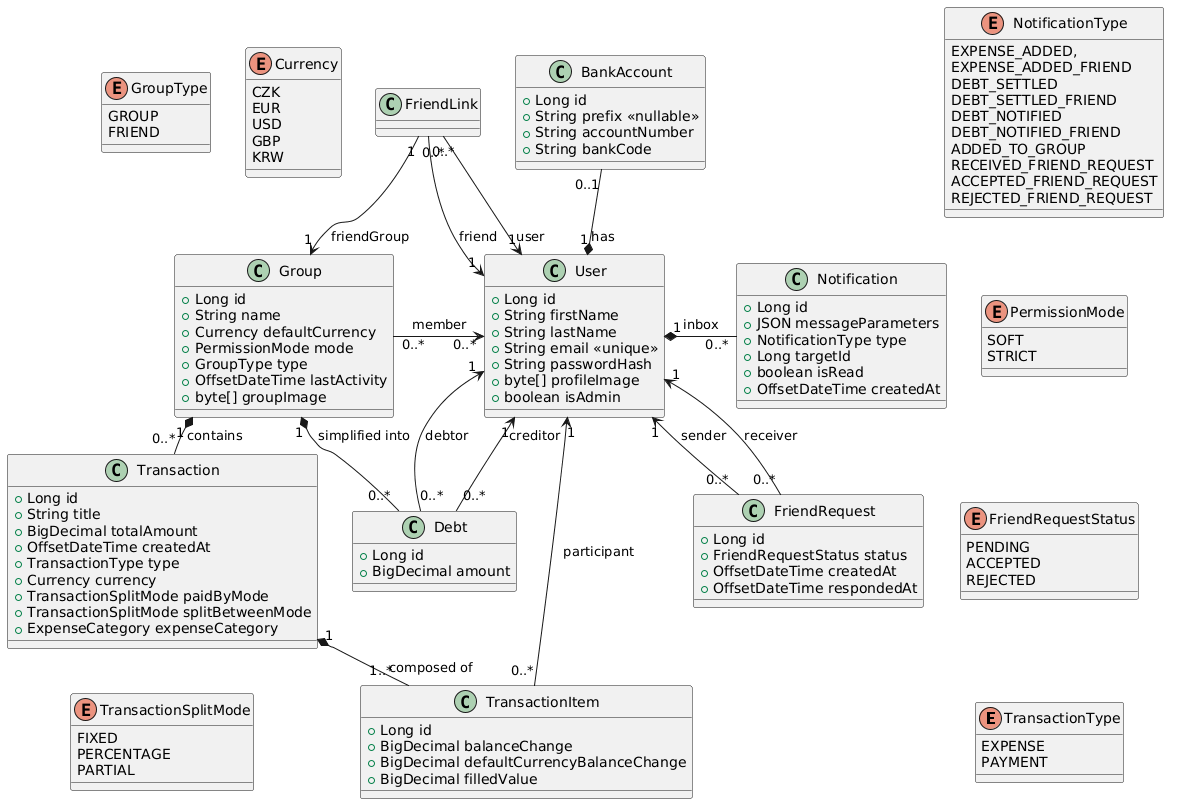
\includegraphics[width=1.05\linewidth]{images/architecture/class_new2.png}
    \caption{UML class diagram featuring core entities of the system}
    \label{fig:class}
\end{figure}

Expenses and payments are merged into a single \emph{Transaction} entity, since they are technically handled the same way. Their only difference is in their business purpose, an expense records a spending, while a payment, on the other hand, serves for settling debts.

Every \emph{Transaction} consists of a number of \emph{Transaction items}. This entity represents the actual effect on a user's balance and is created for every user involved in the transaction. Payers therefore have a positive balance change, and participants have a negative balance change. The sum of all balance changes of a transaction has to be zero. This ensures the advanced expense splitting mentioned in \emph{\hyperref[frq:14]{FRQ14 - Adding an expense}}.

A \emph{Debt} is a helper entity that represents the result of the settlement engine. While a \emph{Transaction} is a permanent history of an event, \emph{Debts} track the current state of ``who owes what to whom'' after simplification. After adding, modifying, or deleting a \emph{Transaction}, all \emph{Debts} in that group are deleted and recalculated, so the group state is always up to date. Although these balances could be computed at runtime and cached, the \emph{Debt} entities are persisted to avoid higher response times and synchronization risks.

For managing non-group expenses (\emph{\hyperref[frq:16]{FRQ16 - Non-group expenses}}), a special Group with the type FRIEND is created for friends. Therefore, the exact same logic that exists in Group can be reused, which is very useful, for example, for counting the overall balance of a user.

\subsection{Component diagram}

A component diagram provides an overview of the structure of the system by decomposing it into high-level functional blocks, components. Every component should have its singular purpose and its own responsibility~\cite{comp}. The component diagram for this application can be seen in~\autoref{fig:comp}.

\begin{figure}[htbp]
    \centering
    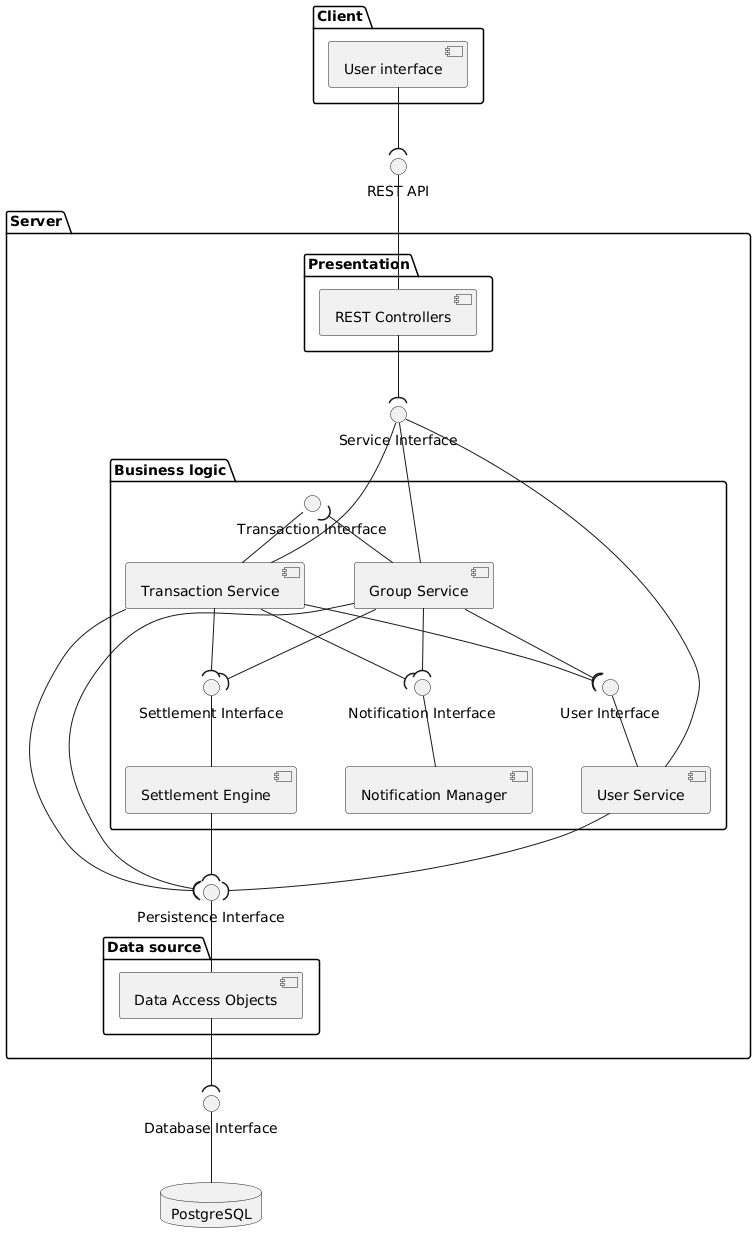
\includegraphics[width=0.75\textwidth]{images/architecture/comp3.png}
    \caption{UML component diagram illustrating the interactions between core parts of the system. For readability, REST controllers and Data Access Objects (DAO) have been grouped into singular components.}
    \label{fig:comp}
\end{figure}

\section{Debt simplification algorithm}
One of the most important parts of the system is the settlement engine. Its main goal is to achieve the lowest number of payments needed to settle all debts in a group. There are two different ways to approach this. The first is the subset sum problem, which is the perfect mathematical approach, always resulting in the absolute minimum number of payments. However, it is very slow for large groups; therefore, a greedy solution is often used as a fast alternative, although it does not always find the optimal solution.

In both options, only the total net balance is important, not individual transactions. Regardless of the algorithm used, the first step is to aggregate all transactions for each member. This divides the group members into two categories: debtors, with a negative balance, and creditors, with a positive balance. If a member has a balance of zero, they are not further involved in the settlement process. The total value of both categories is always equal. \autoref{fig:group-vis} illustrates the transition from a complex network of original transactions to a simple view of the two categories based on their balance. In the diagram, creditors are labeled as ``givers'' and debtors as ``receivers.''

\begin{figure}[h]
    \centering
    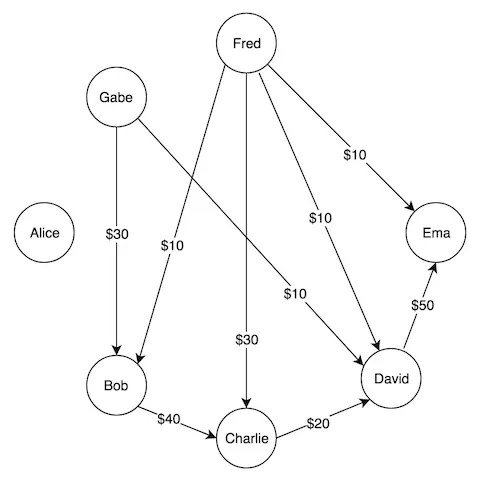
\includegraphics[width=0.45\textwidth]{images/architecture/group1.png}
    \hfill
    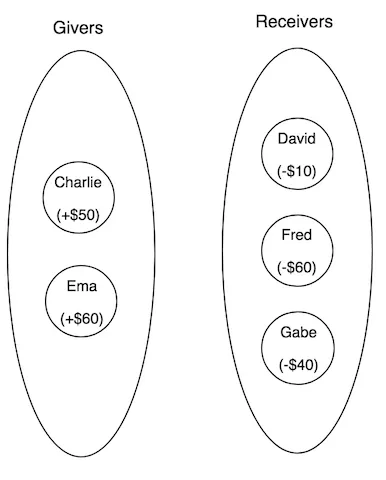
\includegraphics[width=0.45\textwidth]{images/architecture/group2.png}
    \caption{Different visualization of debts in a group~\cite{group-vis}}
    \label{fig:group-vis}
\end{figure}

\subsection{Subset sum problem}
In its general formulation, the subset sum problem involves a set of positive integers $S$ and a target integer $T$. The goal is to determine whether there is a subset $S' \subseteq S$ whose elements sum exactly to $T$~\cite{CLRS}. This problem is known to be NP-complete, which means that there is no known algorithm that can find a solution in polynomial time~\cite{np}.

Debt simplification is a variant of this problem. Instead of a set consisting of only positive integers, negative numbers are also allowed, representing the set of net balances of all group members. The target $T$ is set to zero; we are looking for subsets that have a zero sum. The goal is not to find a single subset, but to partition the group into as many disjoint subsets as possible, each of which sums to zero.

In a group of $n$ members divided into $k$ zero-sum subsets, the entire group can be settled in exactly $n-k$ payments. Therefore, maximizing $k$ is equivalent to minimizing the number of payments. The worst case scenario is $n-1$ payments, when no subset other than the entire group is found.

Since every subset must be checked, this method results in an exponential time complexity of $O(2^n)$. Although this ensures the optimal solution, the computational cost doubles with each additional member, making this method difficult to scale for larger groups.

\subsection{Greedy solution}
Given these scaling challenges, a more efficient alternative is needed. This is where greedy strategy comes in. A greedy algorithm works by making the best possible choice at every step, in the hope that these locally optimal decisions will lead to a globally optimal result~\cite{CLRS}. Although it might not always find the perfect mathematical solution, it is significantly faster. They are used when performance is more important than finding the absolutely best solution. Greedy algorithms provide the outcome that is the best or at least ``good  enough.''

In a group of $n$ members, this algorithm almost always results in $n-1$ payments required to settle the entire group. With the usage of the correct algorithms and data structures, the complete sort with complexity $O(n\ log\ n)$ only needs to be done once at the beginning of the process. Maintaining the order of the remaining members (popping the debtor and the creditor and pushing one of them back) takes only logarithmic time per step and occurs at most $n-1$ times. The total complexity is the sum of the initial sort and the pairing loop, $O(n\ log\ n) + O(n\ log\ n)$ or simply $O(n\ log\ n)$.

\subsection{Selection of the settlement algorithm}
For this application, the greedy approach was chosen primarily for its efficiency, which guarantees high performance even as the number of group members grows. The pseudocode of the algorithm is detailed in \autoref{alg:greedy}.

To justify this decision, a performance testing was conducted to compare the two approaches. The metrics evaluated are the execution time and the number of payments required to settle the group based on the number of members of the group $n$. For every $n$ from 2 to 25, the results represent the average of 20 test runs. The results of this test are shown in \autoref{table:performance_comparison}.

\begin{table}[htbp]
\centering
\caption{Performance comparison between the Greedy (G) and Perfect (P) settlement algorithms containing average execution time [ms] and average number of payments to settle all members of the group.}
\label{table:performance_comparison}
\begin{tabular}{|l|r|r|r|r|}
\hline
\textbf{Size} & \textbf{G-Exec time} & \textbf{P-Exec time} & \textbf{G-Payments} & \textbf{P-Payments} \\
\hline
2  & 0.0083 & 0.0272     & 1.00  & 1.00  \\
3  & 0.0132 & 0.0487     & 2.00  & 2.00  \\
4  & 0.0176 & 0.0873     & 3.00  & 3.00  \\
5  & 0.0210 & 0.1514     & 4.00  & 4.00  \\
6  & 0.0147 & 0.1908     & 5.00  & 5.00  \\
7  & 0.0291 & 0.6397     & 6.00  & 6.00  \\
8  & 0.0369 & 1.0381     & 6.95  & 6.95  \\
9  & 0.0355 & 2.2317     & 7.95  & 7.90  \\
10 & 0.0462 & 4.7962     & 9.00  & 8.75  \\
11 & 0.0510 & 10.2621    & 9.95  & 9.90  \\
12 & 0.0427 & 18.1265    & 10.95 & 10.70 \\
13 & 0.0459 & 37.1334    & 11.90 & 11.20 \\
14 & 0.0499 & 76.8242    & 12.80 & 12.15 \\
15 & 0.0502 & 161.3048   & 13.80 & 12.80 \\
16 & 0.0467 & 274.9712   & 14.65 & 13.75 \\
17 & 0.0420 & 481.0159   & 15.80 & 14.50 \\
18 & 0.0470 & 1 006.2907 & 16.45 & 15.05 \\
19 & 0.0507 & 2 121.0147 & 17.70 & 16.00 \\
20 & 0.0510 & 4 449.9533 & 18.80 & 16.65 \\
21 & 0.0566 & 9 485.1819 & 19.65 & 17.15 \\
22 & 0.0580 & 20 312.6722 & 20.70 & 18.15 \\
23 & 0.0577 & 42 449.3168 & 21.60 & 18.90 \\     
24 & 0.0600 & 87 106.9004 & 22.35 & 19.60 \\
25 & 0.0655 & 181 541.3340 & 23.35 & 20.40 \\ 
\hline
\end{tabular}
\end{table}

The results clearly show that the subset sum variant starts to really struggle around 18 members, taking over one second on average to compute the debts, while only saving approximately one to two payments for the larger groups. The execution time then doubles with every additional member, consistent with its $O(2^n)$ complexity.

Some could argue that in most cases the groups are much smaller than this. Although this is true, the results also show that for these smaller groups, even the greedy algorithm usually finds the most optimal solution (usually $n-1$ payments). The difference in payments becomes noticeable only for large groups, where the perfect algorithm loses in performance. For these reasons, the greedy algorithm was selected for this application.

\begin{algorithm}[h]
\caption{Greedy debt simplification algorithm pseudocode}
\label{alg:greedy}
\begin{algorithmic}
\Require A set of $members$ where each $m \in members$ has a $balance$
\Ensure A series of transactions settling all debts
\State $debtors \gets []$
\State $creditors \gets []$
\For{each $m \in members$}
    \If{$m.balance < 0$}
        \State $debtors.add(m)$
    \ElsIf{$m.balance > 0$}
        \State $creditors.add(m)$
    \EndIf
\EndFor
\State
\State $debtors.sort(ASC)$
\State $creditors.sort(DESC)$
\State
\While{$debtors$ is not empty \textbf{and} $creditors$ is not empty}
    \State $d \gets debtors.pop()$
    \State $c \gets creditors.pop()$
    \State
    \State $amount \gets \min(|d.balance|, c.balance)$
    \State $recordDebt(d, c, amount)$
    \State
    \State $d.balance \gets d.balance + amount$
    \State $c.balance \gets c.balance - amount$
    \State
    \If{$d.balance \neq 0$}
        \State $debtors.insertSorted(d)$
    \EndIf
    \If{$c.balance \neq 0$}
        \State $creditors.insertSorted(c)$
    \EndIf
\EndWhile
\end{algorithmic}
\end{algorithm}

\section{UI/UX Prototype}
To demonstrate the design of the application, the Figma\footnote{Available at: \url{https://www.figma.com/}. Accessed 2025-12-27.} tool     was used to create a high-fidelity user interface prototype. As the application is intended to be used on both mobile and desktop platforms, a high priority is responsiveness; therefore, all screens were created in both views to illustrate how the layout adapts to different screen sizes. This section contains a few key pages, the rest can be seen in \autoref{app:a}.

The interface was designed to match the established usability conventions. This includes, for example, positioning the application logo in the top-left corner, placing the primary menu across the top of the screen, and the secondary menu at bottom-left (e. g. group details tabs). The currently selected menu item is reversed in color to work as a clear ``You are here'' indicator~\cite{DMMT}.

\autoref{fig:homepage} represents the home page of the application. The core components are the menu from which the user can navigate the entire application, a grid with a few groups, and a log with recent activity.

\begin{figure}[htbp]
    \centering
    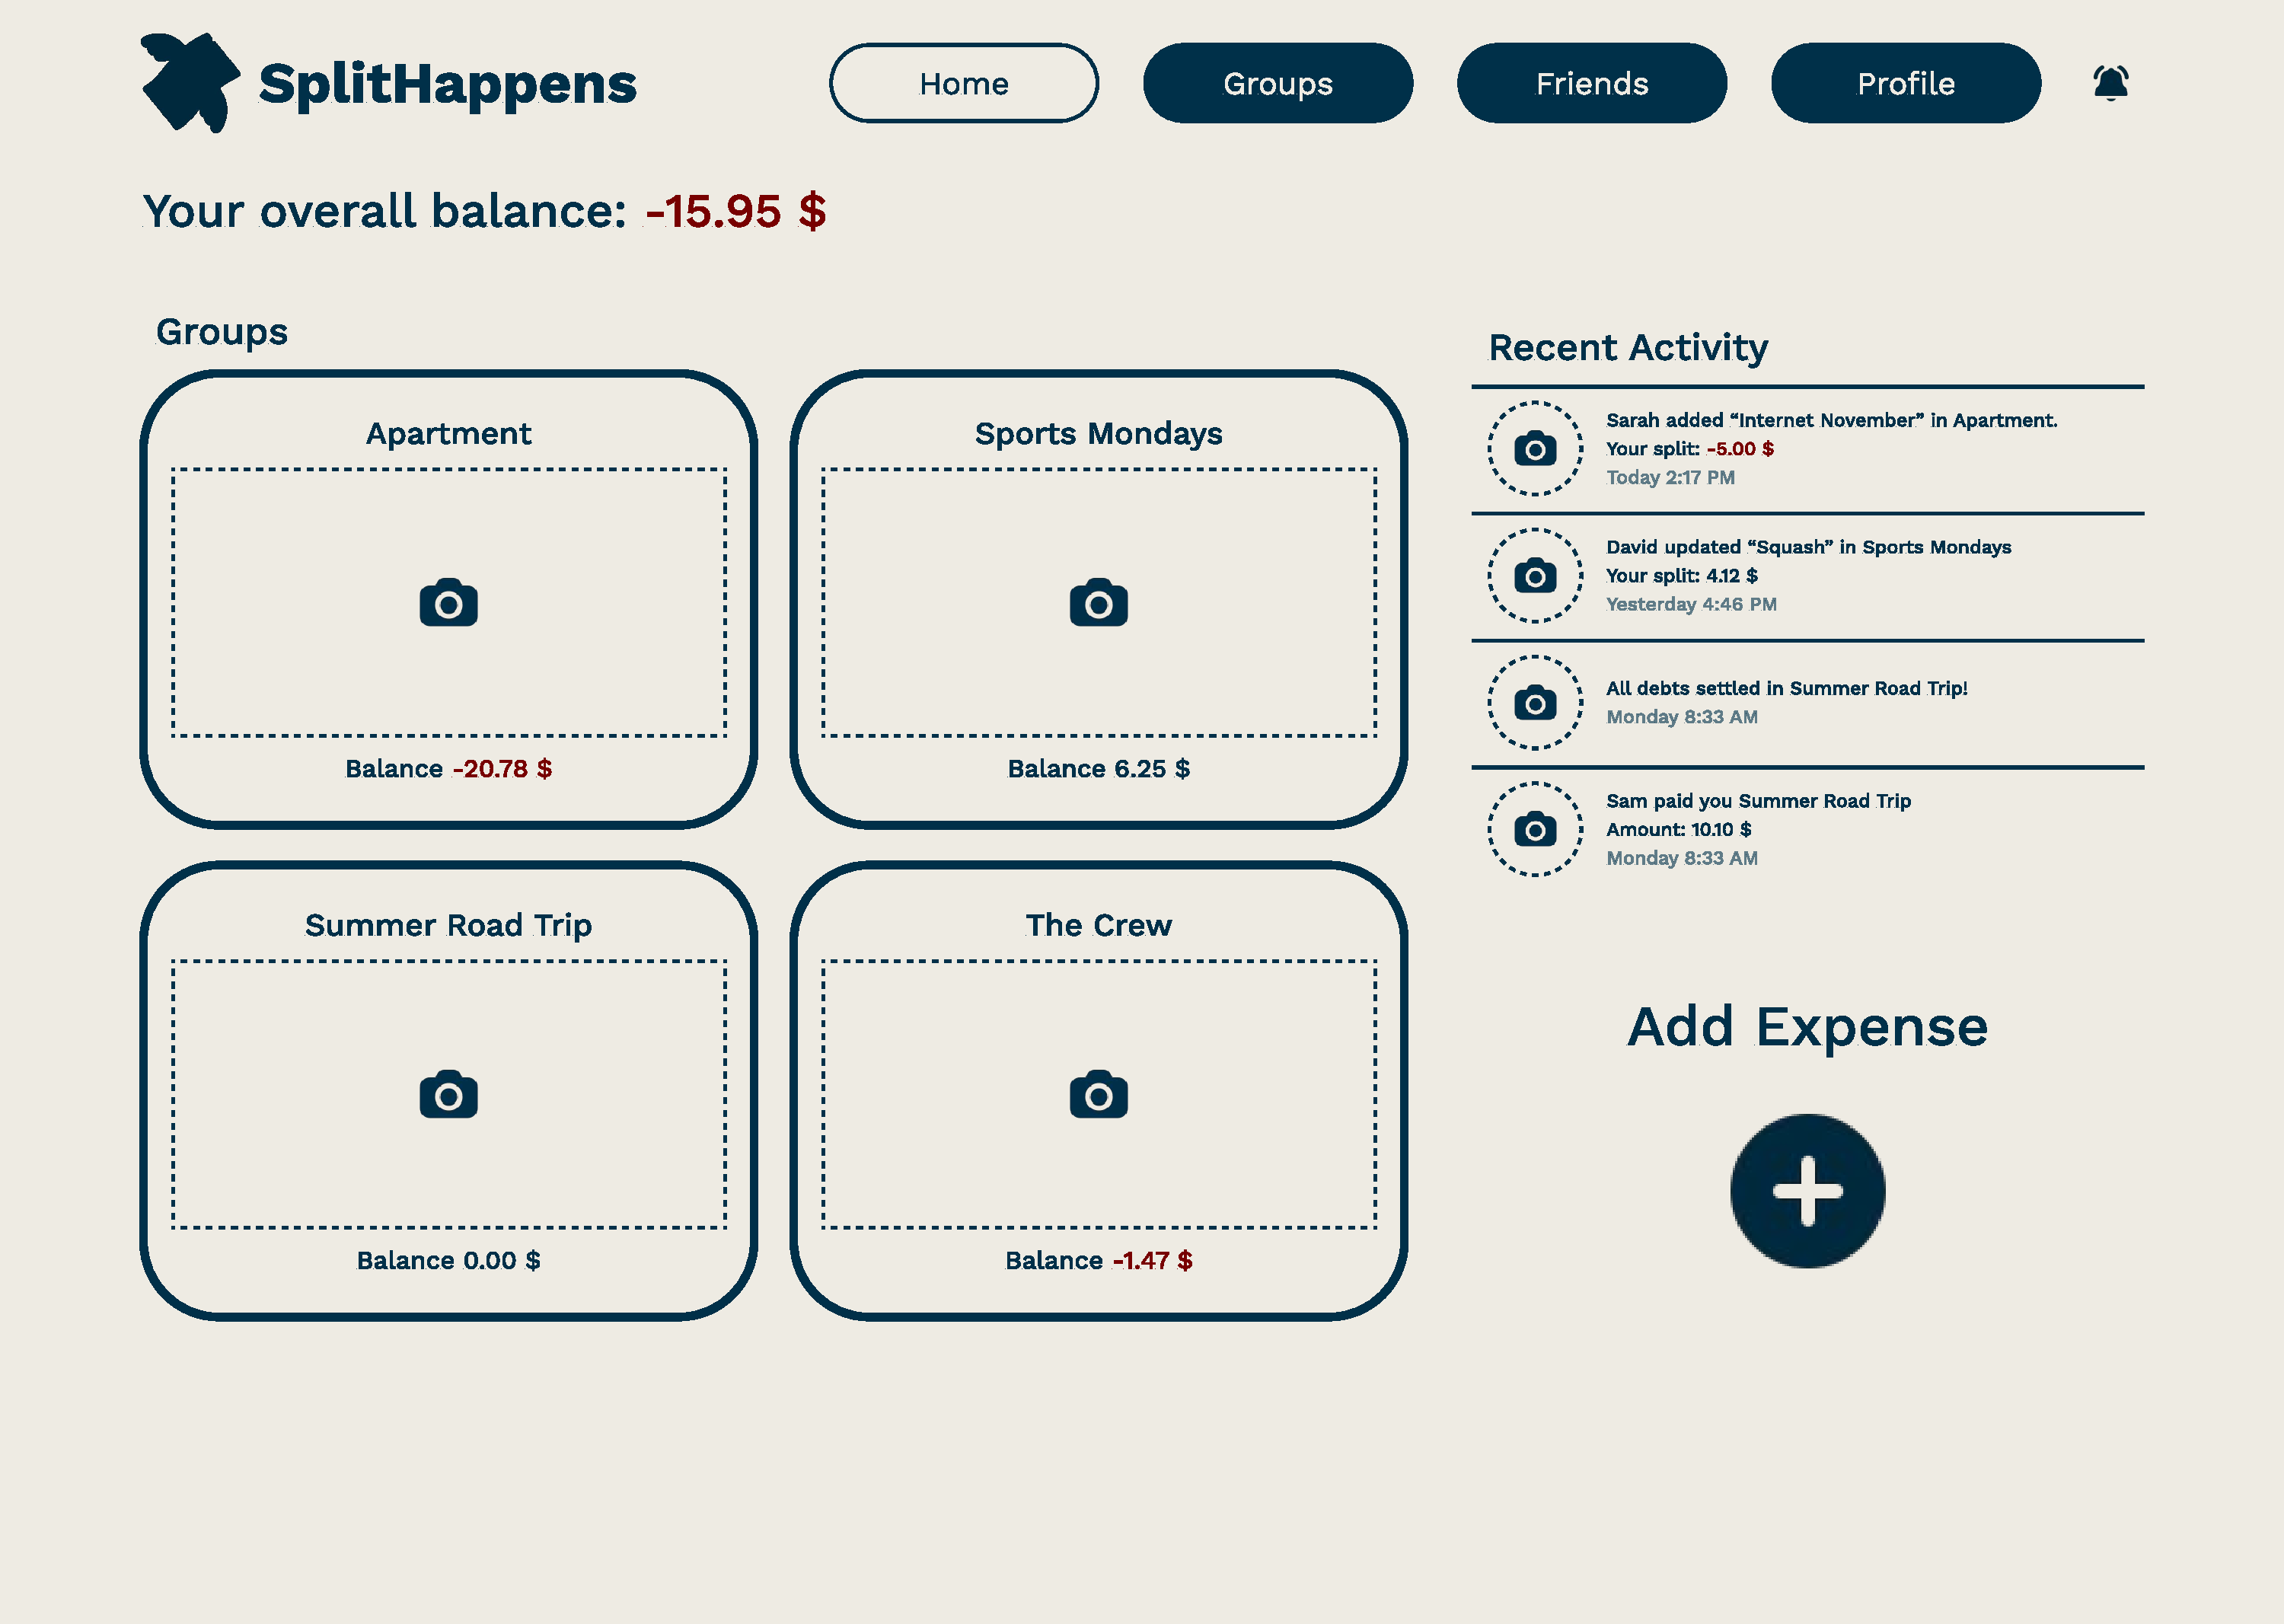
\includegraphics[width=0.9\textwidth]{images/prototype/Homepage.pdf}
    \caption{UI prototype - Desktop home page featuring group cards, recent activity log and quick add expense button}
    \label{fig:homepage}
\end{figure}

The most important feature is adding new expenses. This is showcased in \autoref{fig:add_exp}. The form allows users to split the expense in a very flexible way in multiple modes: by a fixed amount, by parts, or by percentage. Users can also assign a category.

\begin{figure}[hbtp]
    \centering
    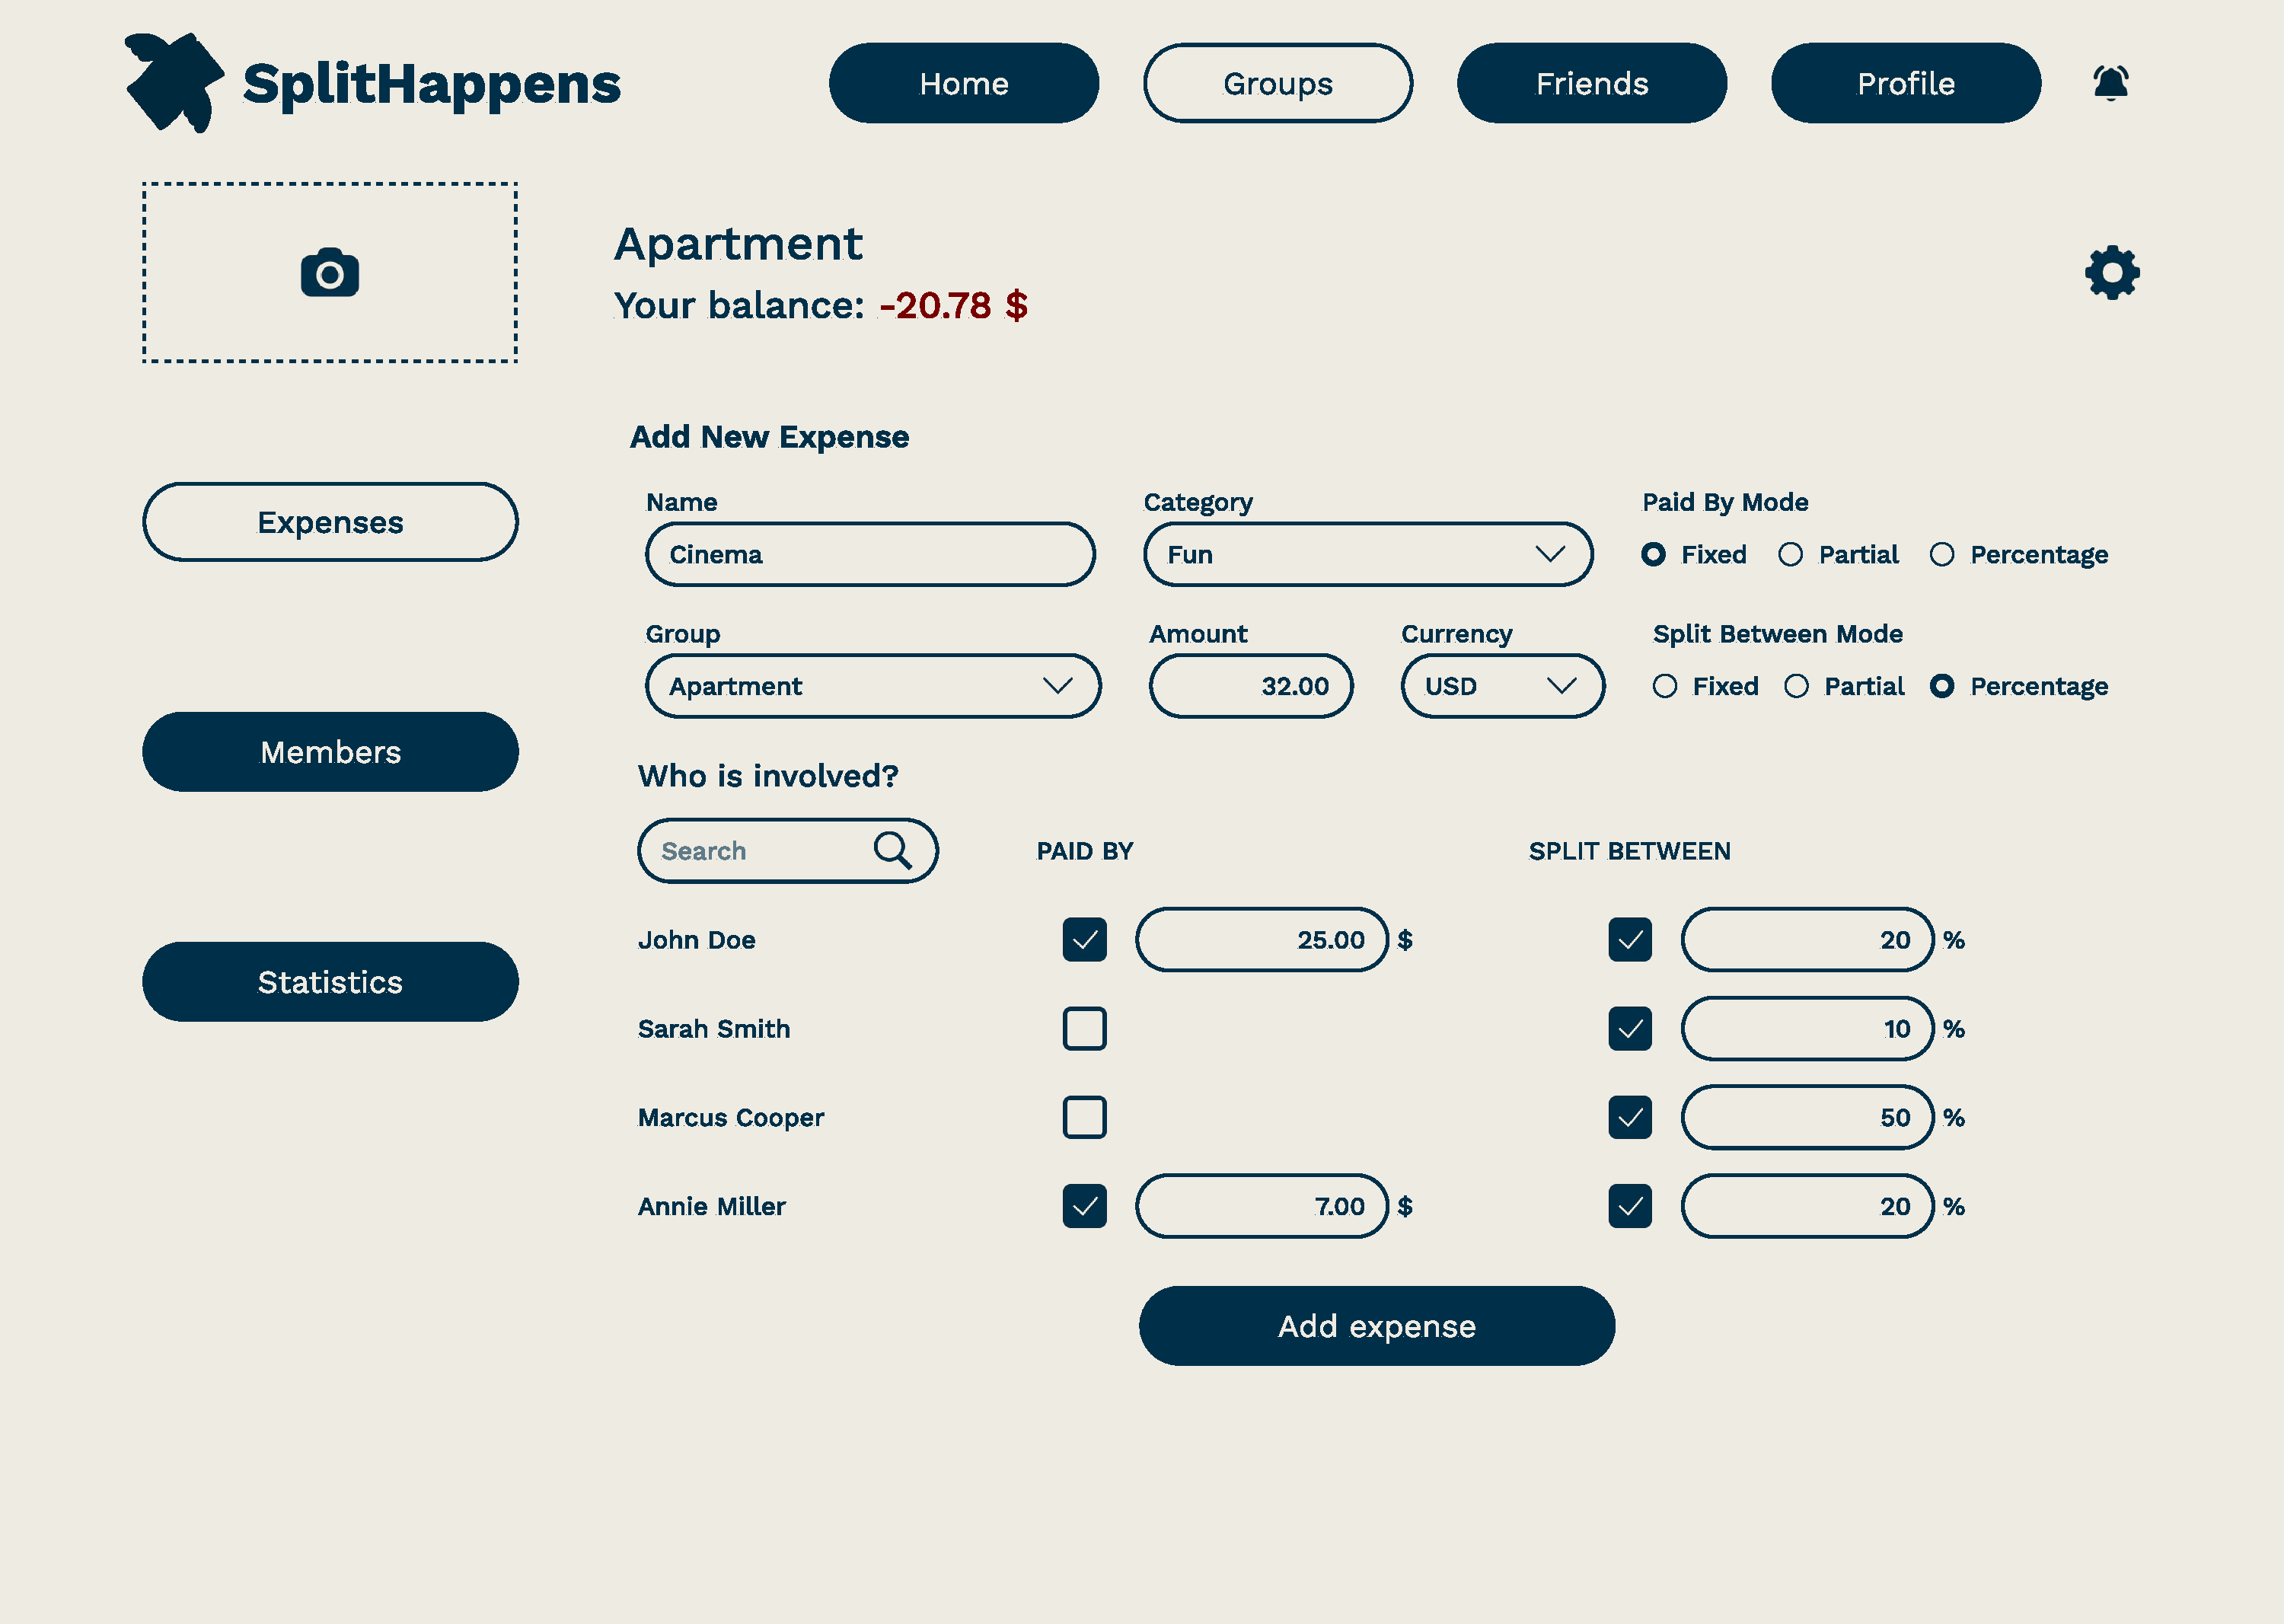
\includegraphics[width=0.9\textwidth]{images/prototype/Group Detail - Add expense.pdf}
    \caption{UI prototype - Add new expense form with example expense that is split between all members by percentages}
    \label{fig:add_exp}
\end{figure}

As an example for a mobile screen, \autoref{fig:mob_members} highlights the list of all group members. After clicking the arrow button on the right, all debts related to that user appear, including buttons to pay the debt, generate a QR code, or remind the debtor, as shown in \autoref{fig:mob_member_balance}.

\begin{figure}
    \centering
    \begin{subfigure}{0.4\textwidth}
        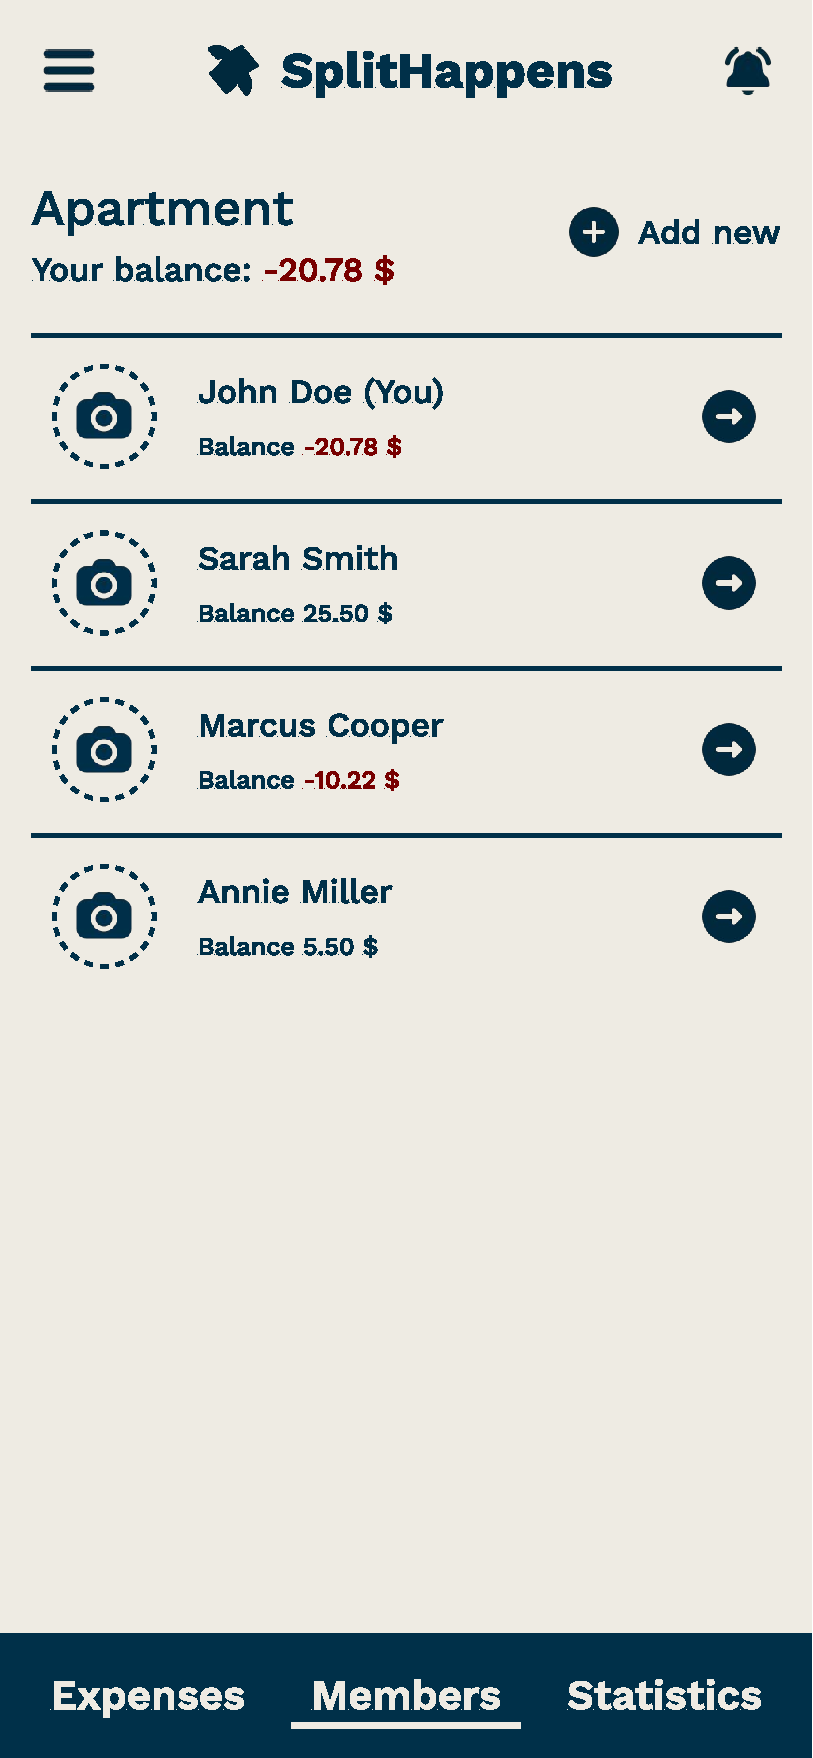
\includegraphics[width=\textwidth]{images/prototype/Mobile Group Detail - Members.pdf}
        \caption{Members list}
        \label{fig:mob_members}
    \end{subfigure}
    \hspace{35pt}
    \begin{subfigure}{0.4\textwidth}
        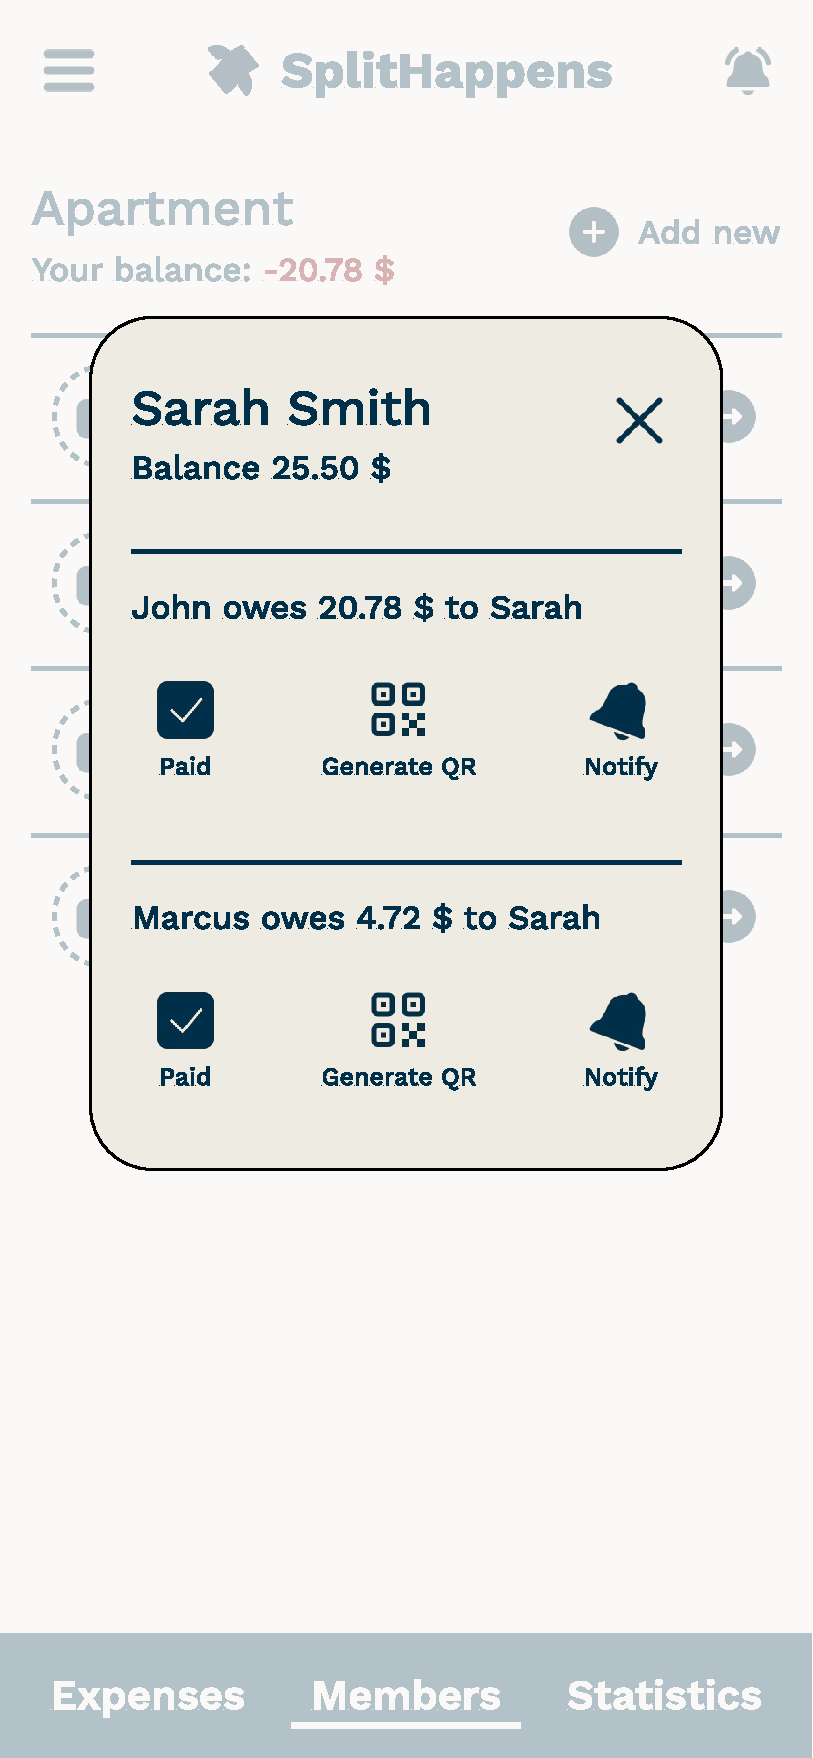
\includegraphics[width=\textwidth]{images/prototype/Mobile Group Detail - Member balances.pdf}
        \caption{Member balance}
        \label{fig:mob_member_balance}
    \end{subfigure}
    \caption{UI prototype - Mobile screen example}
    \label{fig:mobile_example}
\end{figure}

\subsection{Prototype testing}
Based on this prototype, a simple testing with two individuals was conducted before starting the development. The goal was to get feedback on the overall user experience as early as possible in the process, since the cost of change is the lowest at this point in the development. 

This testing raised several important discussion points. Some of these suggestions were immediately applied to the prototype, while others need further investigation and will be addressed during development.
\begin{itemize}
    \item An Add expense button was added to the homepage because it is a primary task and should be easily accessible.
    \item The color palette was also brought up for discussion. The app must provide enough contrast while keeping the design attractive. The color palette might change in the future with more testing.
    \item Button labels were discussed to make the app more intuitive. As a result, some labels were added and some were removed.
    \item The option to filter expenses was missing.
    \item The member balances felt too overwhelming when showing the information and actions buttons for all debts at once. Now, only the debts of the logged-in user are shown right away, while the rest can be displayed via the Show debts button.
    \item The button icon to show more information in mobile view was unified throughout the prototype.
    \item The button to add an expense in the group submenu was hidden to avoid confusion, as there would otherwise be two Add expense buttons, one for creating a new expense and one for submitting the form.
    \item Several minor errors were fixed, such as typos or inconsistent design in shared components.
\end{itemize}

\chapter{Implementation}
Following the architectural and functional design described previously, this chapter details the practical realization of the application. It justifies the selection of the technology stack, covers the deployment process, and explains the specific design patterns applied during development. Finally, the chapter provides an overview of all the successfully implemented features relative to the initial functional requirements. The source code for the application is available at \url{https://gitlab.fel.cvut.cz/sadilsta/split-happens}.

\section{Technology stack}
As established in the design phase, the application follows a layered architecture. The system utilizes PostgreSQL for data persistence, Java with Spring Boot for a secure and scalable backend API, and React for a modular, responsive frontend interface. This core stack is further supported by several specialized tools and libraries.

\subsection{Database}
PostgreSQL was selected as the relational database management system for the application. This technology is currently the most popular choice among developers globally~\cite{postgresql}. Due to this and its unmatched strict transactional integrity, it was chosen over other alternatives such as MySQL.

\subsection{Backend}
Java, specifically utilizing the Spring Boot framework, remains a leading choice for enterprise applications due to its long-standing reputation for stability and security in core infrastructure~\cite{java}. These advantages, along with the developer's previous experience with the language, made Java the definitive choice for the backend.

The backend functionality is supported by several specialized libraries, tools, and frameworks chosen to handle infrastructure requirements such as database versioning, security, and API documentation.
\begin{itemize}
    \item \textbf{Spring Boot} - As the de facto industry standard for modern Java development, this framework provides the infrastructure and orchestration of the application, like managing security or database connectivity. It simplifies development through automatic configuration, removing the overhead of manual boilerplate setup. In addition, its use of starter dependencies ensures that all required libraries are compatible and correctly versioned~\cite{springboot}. This allows development to remain focused on the core business logic and specific requirements of the application.
    \item \textbf{Liquibase} - Liquibase is an open-source database version control tool that manages schema changes by recording every modification in a centralized, state-aware changelog. It ensures that the PostgreSQL database structure remains synchronized across all environments, allowing for automated and repeatable deployments without the risk of manual error or schema inconsistencies~\cite{liquibase}.
    \item \textbf{JWT} - User authorization is managed through JSON Web Tokens. This standard (RFC 7519) defines a compact way to securely transmit information between the client and the server~\cite{jwt}. It provides a stateless authorization, where the token carries verified claims of the user, eliminating the need for server-side session storage.
    \item \textbf{OpenAPI} - REST endpoints are described using the OpenAPI specification, a language agnostic standard that provides a formal definition of the API's structure and behavior, and the associated DTOs (Data Transfer Object)~\cite{openapi}.
    \item \textbf{MapStruct} - This compile-time code generation library automates the mapping between database entities and Data Transfer Objects (DTOs)~\cite{mapstruct}. It reduces boilerplate code while helping to maintain a clean separation of concerns, ensuring that the database schema is not directly exposed through the REST API.
\end{itemize}

\subsection{Frontend}
For the client-side, React was selected primarily for its component-based approach and a relatively accessible learning curve. In addition, it is also a very popular option within the industry~\cite{react}, making it a clear choice for developing modern web applications.

The following tools and libraries were integrated to support the frontend infrastructure:
\begin{itemize}
    \item \textbf{TanStack React Query} - This library serves data management purpose, handling asynchronous data fetching, caching, and synchronization with the REST API. That is crucial due to loading states and background updates that require the UI to remain consistent with the backend data~\cite{tanstack}. 
    \item \textbf{QR codes API} - The application uses an external API to generate payment QR codes that conform to established Czech banking specifications~\cite{qr}. This integration enables a low-effort payment process by allowing users to scan the code with a mobile banking application, reducing the risk of manual entry errors.
    \item \textbf{Zod} - This library is used as a schema declaration and validation tool, which is critical for the application's complex parts, such as the add expense form. Zod provides runtime verification of user input before processing by the backend.
    \item \textbf{React Intl} - To address the requirement for multi-currency support, React Intl was integrated to standardize formatting, like showing currency symbols or balances accurately across different group contexts.
    \item \textbf{Material UI} - MUI is a comprehensive component library that implements the Material Design system. It provides a consistent, responsive user interface by reusing prebuilt UI components~\cite{mui}.
\end{itemize}

\section{Deployment}
The application is designed according to a three-tier containerized architecture. The individual components — the database, backend, and frontend — are decoupled and independent. This approach allows the system to be deployed in different environments, from a single local server to a distributed cloud infrastructure.

These independent modules are linked via standardized protocols, specifically JDBC for the database and REST over HTTPS for client-server communication. These connections are established at runtime using environment variables to inject the necessary hostnames, connection strings, and security credentials.

The application's production environment is currently divided into three distinct hosting providers, which were selected primarily for the availability of a functional free tier and previous experience with the platforms.
\begin{itemize}
    \item \textbf{Database} - The PostgreSQL database is hosted on Neon\footnote{Available at: \url{https://neon.com/}. Accessed 2026-04-26.}, a serverless cloud database platform. Two different database instances were used during development to separate the development and production environments.
    \item \textbf{Backend} - The Java Spring Boot application is deployed on Render\footnote{Available at: \url{https://render.com/}. Accessed 2026-04-26.} as a containerized service. The deployment process builds a Docker image, which is then stored in a Docker Hub repository, from which Render pulls and deploys the image.
    \item \textbf{Frontend} - The React frontend is hosted on Vercel\footnote{Available at: \url{https://vercel.com/}. Accessed 2026-04-26.}, using the Vercel CLI to handle the compilation and deployment. The application can be accessed via this link \url{https://splithappens-fel.vercel.app/}.
\end{itemize}

\subsection{CI/CD}
The project implements a Continuous Integration and Continuous Deployment pipeline using GitLab CI/CD. The pipeline is triggered automatically on every commit and is organized into four stages:
\begin{itemize}
    \item \textbf{Build} - Compiles and builds the backend and frontend separately.
    \item \textbf{Test} - Runs the automated tests and creates a coverage report.
    \item \textbf{Publish (main branch only)} - Creates a Docker image and pushes it to Docker Hub.
    \item \textbf{Deploy (main branch only)} - Notifies Render via a webhook to pull and run the latest container image, and deploys the frontend using the Vercel CLI.
\end{itemize}

\section{Design patterns}
The \textbf{Strategy} is utilized to define a family of algorithms, encapsulate each one, and make them interchangeable. It is used when related classes differ in their behavior~\cite{gof}. This application offers three different modes for splitting an expense: fixed amounts, partial shares, and percentages. Each of these modes is assigned a split strategy which then calculates the actual balance change for every involved group member.

The \textbf{Facade} design pattern provides a unified, higher level interface to a complex set of functionalities, making it easier to use from the outside~\cite{gof}. In this application, the settlement engine serves as a facade by hiding all the complexities of the simplification algorithm behind a single, simplified method.

\section{Implemented features}
To deliver a functional system within the project's schedule, the implementation phase focused on developing features based on their priority, defined in~\autoref{table:frq}. From the set of described features, all functional requirements categorized as Core and Important have been successfully completed, which means that the application is fully functional for its primary purpose. Regarding the Enhancement category, these features were implemented selectively based on their impact and the required development time. Specifically, the implemented Enhancement features are \emph{\hyperref[frq:29]{FRQ29 - Notifications}} and \emph{\hyperref[frq:30]{FRQ30 - Sending a reminder}}. The overview of all the features implemented is provided in \autoref{table:impl}.

\begin{table}[ht!]
\centering
\begin{tabularx}{\textwidth}{|X|p{2.7cm}|l|}
\hline
\textbf{Requirement} & \textbf{Priority group} & \textbf{Priority} \\ \hline

\rowcolor{green!15} FRQ01 - Registration & Core & 10 \\ \hline
\rowcolor{green!15} FRQ02 - Authentication and authorization & Core & 10 \\ \hline
\rowcolor{green!15} FRQ08 - Group viewing & Core & 10 \\ \hline
\rowcolor{green!15} FRQ11 - Group detail & Core & 10 \\ \hline
\rowcolor{green!15} FRQ14 - Adding an expense & Core & 10 \\ \hline
\rowcolor{green!15} FRQ15 - Expense detail & Core & 10 \\ \hline
\rowcolor{green!15} FRQ22 - Personal balance & Core & 10 \\ \hline
\rowcolor{green!15} FRQ23 - Debt simplification algorithm & Core & 10 \\ \hline
\rowcolor{green!15} FRQ24 - Recording a payment & Core & 10 \\ \hline
\rowcolor{green!15} FRQ03 - User management & Core & 9 \\ \hline
\rowcolor{green!15} FRQ04 - Edit a profile & Core & 9 \\ \hline
\rowcolor{green!15} FRQ09 - Group management & Core & 9 \\ \hline
\rowcolor{green!15} FRQ12 - Add members to a group & Core & 9 \\ \hline
\rowcolor{green!15} FRQ21 - Expense editing and deletion & Core & 9 \\ \hline
\rowcolor{green!15} FRQ05 - User listing and search & Core & 8 \\ \hline
\rowcolor{green!15} FRQ13 - Leaving a group & Core & 8 \\ \hline
\rowcolor{green!15} FRQ20 - Expense filtering and search & Core & 8 \\ \hline

\rowcolor{green!15} FRQ18 - Expense categories & Important & 7 \\ \hline
\rowcolor{green!15} FRQ26 - Generating QR codes & Important & 7 \\ \hline
\rowcolor{green!15} FRQ06 - Adding a friend & Important & 6 \\ \hline
\rowcolor{green!15} FRQ07 - Friend request handling & Important & 6 \\ \hline
\rowcolor{green!15} FRQ27 - Group statistics & Important & 6 \\ \hline
\rowcolor{green!15} FRQ16 - Non-group expenses & Important & 5 \\ \hline

\rowcolor{green!15} FRQ29 - Notifications & Enhancement & 4 \\ \hline
\rowcolor{red!15}   FRQ19 - Custom categories & Enhancement & 3  \\ \hline
\rowcolor{red!15}   FRQ25 - Multi-group friend debt settling & Enhancement & 3  \\ \hline
\rowcolor{green!15} FRQ30 - Sending a reminder & Enhancement & 3 \\ \hline
\rowcolor{red!15}   FRQ17 - Multi currency support & Enhancement & 2  \\ \hline
\rowcolor{red!15}   FRQ28 - User statistics & Enhancement & 2  \\ \hline
\rowcolor{red!15}   FRQ10 - Group permissions & Enhancement & 1  \\ \hline

\end{tabularx}
\caption{Overview of functional requirements and implementation progress. Features highlighted in green are completed, while red background indicates not implemented features.}
\label{table:impl}
\end{table}

\chapter{Testing}
This chapter describes the testing of the developed SplitHappens application. It explains automated tests used and integrated into the CI/CD pipeline, followed by the results and feedback from user testing.

\section{Automated tests}
To make sure that the application remains reliable and easy to maintain as it grows, a suite of automated tests was developed that combine unit tests to verify isolated logic with integration tests to check the full API flow. These tests are integrated into the GitLab CI pipeline and are executed automatically on every commit to verify that no regressions are introduced during the development process.

\subsection{Unit tests}
Unit testing is a fast, low-level practice used to verify isolated business logic without relying on the full application runtime. Unit tests for this application focus primarily on the backend service layer, where the core domain rules live, and on components that are easy to validate independently, such as security-related logic or split computation strategies. 

\subsection{Integration tests}
Unlike unit tests, integration tests validate the behavior of the entire backend, from the presentation layer downward. For this application, the main focus of integration testing was the Transaction, User, and Auth controllers. The tests validate that the endpoints behave correctly as a whole, including request validation, authentication and authorization behavior, and correct HTTP response codes.

\subsection{Code coverage}
Code coverage is tracked using the JaCoCo plugin. The coverage report provides a practical overview of which areas are well-tested, starting from package level down to individual methods. The backend of this application achieves 85\% line coverage. The report is also generated during the test stage of the GitLab pipeline.

\section{User testing}
In addition to automated tests, the developed application has undergone user testing. This section introduces the group of participants and the testing process, followed by the scenarios and feedback received.

\subsection{Testing group}
The testing group consisted of twelve participants, providing a diverse spread in terms of age and professional background. Nine of them were university students (aged 22-26) of various disciplines, such as IT, architecture, law, or marketing. The remaining three participants represented a more senior generation (aged 55-57). Although the professional background differs, all participants are daily users of digital technology.

\subsection{Testing process}
For the testing itself, five test scenarios were defined to test the functionality of the application. Each scenario consists of a short set of tasks that testing participants must complete. The scenarios were intentionally kept simple with no extra guidance to simulate the experience of real users navigating the interface and finding specific features. All scenarios are detailed in \autoref{app:b}.

User testing was conducted in two rounds. The first included scenarios 1 through 3, while the remaining two scenarios were tested in the second round. The testing itself was performed either on a video call where immediate feedback could be provided or asynchronously based on written instructions. Nine of the participants completed the scenarios on desktop devices, while the rest tested on mobile phones to test the responsiveness of the application as well. The participants recorded the time taken to complete the scenario.

After completing each testing scenario, participants were asked to fill out a form on how long it took them to finish the scenario and answered two closed questions on a scale of 1 (easy to use, intuitive) to 5 (difficult to use, unintuitive). These questions focused on how easy it was to complete the task and how intuitive the app felt. Finally, a couple of open questions allowed participants to include any further comments on how to improve the application or if they got stuck somewhere in the scenario.

The test scenarios are the following:
\begin{enumerate}
    \item \textbf{User management} - Participants were asked to create an account and personalize it by uploading a profile image.
    \item \textbf{Group management} - This scenario involved group related tasks, like creating a new group or managing its members.
    \item \textbf{Expenses and payments} - This is the core workflow, users added shared expenses, generated QR codes, and recorded payments.
    \item \textbf{Friends} - This scenario focused on friends, requiring participants to send or respond to friend requests and add non-group expenses.
    \item \textbf{Statistics and Notifications} - Participants review their spending through the application's data visualization and evaluate real-time event notifications.
\end{enumerate}

\subsection{Results}
This section presents the results of the user testing. For all scenarios, a summary of the average completion time and the average scores from the scaled questions is provided in~\autoref{table:usertesting}. Additionally, each scenario is discussed in more detail, including qualitative feedback from the open questions and addressing functional or UI/UX improvements.

\begin{table}
\centering
\begin{tabularx}{\textwidth}{|X|l|l|l|}
\hline
\textbf{Scenario} & \textbf{Avg. time} & \textbf{Ease of use} & \textbf{Intuitiveness} \\ \hline

User management              & 02:20 & 1.13 & 1.33 \\ \hline
Group management             & 02:34 & 1.54 & 1.75 \\ \hline
Expenses and payments        & 06:34 & 2.54 & 2.00 \\ \hline
Friends                      & 02:46 & 1.71 & 1.75 \\ \hline
Statistics and Notifications & 03:12 & 1.04 & 1.08 \\ \hline

\end{tabularx}
\caption{Overview of the quantitative results of the user testing.}
\label{table:usertesting}
\end{table}

\subsubsection{Test Scenario 1 - User management}
The first scenario was very clear for users, achieving fast completion times and strong ease of use and intuitiveness ratings.

Despite the positive results, the participants pointed out some areas where the interface could be improved. Specifically, it was unclear during the registration that certain fields were related to a bank account, especially the Prefix field. To address this, a heading was added to clearly indicate that these fields belong to bank account information. Despite being a widely recognized convention, a legend explaining that an asterisk marks a mandatory field was added. The users also reported the absence of a language switcher (EN/CS) in the registration and login forms. Finally, some of the participants found the Edit Profile pencil icon too small, so it was made larger for better visual clarity.

\subsubsection{Test Scenario 2 - Group management}
The second scenario achieved slightly lower ratings than the first, primarily due to a usability issue reported by multiple participants. Many users found the action to add members to a group to be unintuitive, which resulted in one user not being able to complete the scenario at all. To resolve this, a dedicated button was added, visible at all times on the group details page.

\subsubsection{Test Scenario 3 - Expenses and payments}
Given its complexity and importance to the application, the third scenario received the most extensive feedback and required the longest time for participants to complete.

The primary feedback focused on the expense management forms. Users suggested that the Add expense form should, by default, automatically split the total amount equally among all involved group members, for both payers and participants. These calculated splits can, of course, be overridden by manual action, which then excludes the modified values from following automatic calculations. Additionally, several issues were identified in the Edit expense flow. The split data was not prefilled correctly because the selected ``Split'' or ``Paid by'' modes were not being persisted, requiring users to manually select and fill the data again. To address this, the transaction backend entity was extended to include these modes, and the frontend form was refined to show all the data correctly. To assist users with the various splitting modes, informational helpers were added to explain Fixed, Partial, and Percentage splits. Finally, the category field was made optional, defaulting the expense to category OTHER if none is provided.

The settlement and payment process was also improved based on reports that the Settle action was difficult to find. Therefore, the Members tab on the group detail page was renamed to Balances to better guide the users to their current debts. To prevent accidental settlements, a confirmation modal was added. Finally, the QR code generation feature was enhanced by adding the option to save the QR code, allowing users to store or share it as needed.

\subsubsection{Test Scenario 4 - Friends}

The users identified several issues, such as the absence of a back button to navigate from the friend detail view back to the friend list. Another suggestion was to separate incoming and outgoing friend requests to make accepting friend requests more intuitive. The participants also noted that the option to remove a friend from the friend detail view was missing, as it was only available from the friend list interface. An issue similar to the accidental settling of debts was also identified regarding the removal of friends; to address this, a confirmation modal was added.

\subsubsection{Test Scenario 5 - Statistics and Notifications}

Statistics and notifications encountered only a few minor problems. The graph types used were discussed, specifically pie charts versus bar charts, as human perception of pie charts is often inaccurate. 

Regarding notifications, users suggested that clicking on an added expense notification should open the expense details, rather than just the group where the expense was added. The received friend request notification also seemed that users were already accepting the request by clicking the ``Mark as read'' check icon.

\subsubsection{General}
Across all scenarios, participants who tested on mobile devices recorded approximately 22\% longer completion times and also reported slightly worse ratings compared to the average. This included especially the add expense form, where fitting so many input fields on such a small screen proved to be more challenging.

It is also worth noting that during the second round of testing (scenarios 4 and 5), users provided highly positive feedback regarding the automatic calculation of splits, as this simplified the part of the process that users previously found the most demanding.

\chapter{Conclusion}
The core problem in this thesis is the complexity of manual shared group expenses. Firstly, the need for an automated solution was justified.

The development process followed a structured methodology, starting with the analysis of user stories, functional requirements, and a comparison of existing similar applications, such as Splitwise or Tricount. During the design phase, the architecture of the system was defined, and a high-fidelity UI prototype was created to propose a responsive user interface for both desktop and mobile platforms. Finally, the SplitHappens application was implemented using a technology stack consisting of PostgreSQL, Java with Spring Boot, and React.

The settlement engine implements a greedy algorithm to achieve the lowest number of payments required to settle the group. It focuses on the total net balance of each member, rather than the specific transactions. The algorithm usually returns $n-1$ payments, where $n$ is the number of members of the group.

The assignment of the thesis is considered successfully completed as the application meets its primary objectives. Although not all functional requirements were implemented, thanks to the priority based approach, only a small number of secondary functions are left unfinished.

Finally, SplitHappens underwent user testing that involved twelve participants of various backgrounds. This testing provided vital feedback, which is very valuable for future development.

\section{Future steps}
Regarding the already mentioned future development, there is a lot of room to grow, starting with the uncompleted low priority requirements defined in this thesis. This includes custom categories, multi-currency support (in one group), user statistics, and group permissions. The friend relation can aggregate debt data from mutual groups, allowing friends to settle in multiple groups at once. The user interface could also be further improved by adding skeleton screens for loading components, instead of just simple loading text.

Several other nice-to-have features were pointed out by users during testing. This was for example group invite links, which would make it easier to add new members to group, or an expense image upload feature, allowing users to attach pictures to expenses (e.g. receipts).

\begin{thebibliography}{1}
\bibitem{US1} VISUAL PARADIGM. \emph{What is User Story?} Online. Available at: https://www.visual-paradigm.com/guide/agile-software-development/what-is-user-story/. [accessed 2025-11-11].
\bibitem{US2} SCALED AGILE FRAMEWORK. \emph{Story.} Online. 2025-01-27. Available at: https://framework.scaledagile.com/story. [accessed 2025-11-11].
\bibitem{US3} REHKOPF, Max. \emph{User stories with examples and a template.} Online. Available at: https://www.atlassian.com/agile/project-management/user-stories. [accessed 2025-11-11].
\bibitem{US4} MOUNTAIN GOAT SOFTWARE. \emph{User stories.} Online. 2025-10-28. Available at: https://www.mountaingoatsoftware.com/agile/user-stories. [accessed 2025-11-11].
\bibitem{Epic} PRODUCTBOARD. \emph{What is an Epic in agile?} Online. Available at: https://www.productboard.com/glossary/epics/. [accessed 2025-11-11].
\bibitem{FR1} PAVLENKO, Maria. \emph{Functional Requirements in Software Development: Types and Best Practices.} Online. 2023-07-20. Available at: https://www.altexsoft.com/blog/functional-requirements/. [accessed 2025-11-24].
\bibitem{FR2} INTERACTION DESIGN FOUNDATION. \emph{Functional Requirements.} Online. Available at: https://www.interaction-design.org/literature/topics/functional-requirements. [accessed 2025-11-24].
\bibitem{Split1} PANGREKAR, Aditi. \emph{Seven of the best money-splitting apps.} Online. 2024. Available at: https://uk.finance.yahoo.com/news/best-money-splitting-apps-060025118.html. [accessed 2025-10-28].
\bibitem{Split2} GOOGLE LLC. \emph{Splitwise.} Online. Available at: https://play.google.com/store/apps/details?id=com.Splitwise.SplitwiseMobile. [accessed 2025-10-28].
\bibitem{Split3} TRUSTPILOT GROUP PLC. \emph{Splitwise Reviews.} Online. Available at: https://www.trustpilot.com/review/splitwise.com. [accessed 2025-10-28].
\bibitem{Tri1} PARAB, Pranay. \emph{The Five Best Free Alternatives to Splitwise.} Online. 2024-02-19. Available at: https://lifehacker.com/tech/best-free-splitwise-alternatives. [accessed 2025-11-24].
\bibitem{Tri2} TRICOUNT. \emph{Discover all the features.} Online. Available at: https://tricount.com/expense-tracker-features. [accessed 2025-11-24].
\bibitem{Tri3} TRICOUNT. \emph{Automatic Expense Tracking with Your Free tricount Card.} Online. Available at: https://tricount.com/free-credit-card. [accessed 2025-11-27].
\bibitem{SettleUp1} BAYRAK, Nazlinur. \emph{Best Bill-Splitting Apps in 2025.} Online. 2024-03-16. Available at: https://globalfintechmarket.com/blog/best-bill-splitting-apps/. [accessed 2025-11-28].
\bibitem{SettleUp2} SETTLE UP. \emph{Settle Up Premium.} Online. Available at: https://settleup.app/premium. [accessed 2025-11-30].
\bibitem{fundamentals} RICHARDS, Mark and FORD, Neal. \emph{Fundamentals of Software Architecture: An Engineering Approach.} O'Reilly Media, 2020. ISBN 978-1492043454.
\bibitem{clientserver} MOLLOY, Joseph. \emph{Guide to Client-server Architecture or Model.} Online. Available at: https://www.liquidweb.com/blog/client-server-architecture/. [accessed 2025-12-22].
\bibitem{patterns} FOWLER, Martin. \emph{Patterns of Enterprise Application Architecture.} Addison-Wesley, 2002. ISBN 0321127420.
\bibitem{comp} VISUAL PARADIGM. \emph{What is Component Diagram?} Online. Available at: https://www.visual-paradigm.com/guide/uml-unified-modeling-language/what-is-component-diagram/. [accessed 2025-12-22].
\bibitem{group-vis} MOHAN, Mithun. \emph{Algorithm Behind Splitwise’s Debt Simplification Feature.} Online. 2019-12-19. Available at: https://medium.com/@mithunmk93/algorithm-behind-splitwises-debt-simplification-feature-8ac485e97688. [accessed 2025-12-27].
\bibitem{CLRS} CORMAN, Thomas H.; LEISERSON, Charles E.; RIVEST, Ronald L. and STEIN, Clifford. \emph{Introduction to Algorithms.} 3rd. The MIT Press, 2009. ISBN 9780262033848.
\bibitem{np} GAREY, Michael R. and JOHNSON, David S. Computers and Intractability: A Guide to the Theory of NP-Completeness. W. H. Freeman, 1979. ISBN 0716710455.
\bibitem{DMMT} KRUG, Steven. \emph{Don’t Make Me Think, Revisited: A Common Sense Approach to Web Usability.} 3rd. New Riders, 2014. ISBN 0321965515.
\bibitem{postgresql} STACK OVERFLOW. \emph{2025 Stack Overflow Developer Survey.} Online. Available at: https://survey.stackoverflow.co/2025/technology. [accessed 2026-04-26].
\bibitem{java} BJIT. \emph{7 Reasons Why Java Remains the Best Choice for Software Development in 2025.} Online. 2025. Available at: https://bjitgroup.com/blog-details/7-reasons-why-java-remains-the-best-choice-for-software-development-in-2025. [accessed 2026-04-26].
\bibitem{springboot} C. Walls. \emph{Spring Boot in Action.} Manning Publications,
2015. ISBN 9781617292545.
\bibitem{liquibase} LIQUIBASE. \emph{How Liquibase Works.} Online. Available at: https://www.liquibase.com/how-liquibase-works. [accessed 2026-04-26].
\bibitem{jwt} AUTH0. \emph{JSON Web Tokens.} Online. Available at: https://auth0.com/docs/secure/tokens/json-web-tokens. [accessed 2026-04-26].
\bibitem{openapi} OPENAPI INITIATIVE. \emph{What is OpenAPI?} Online. Available at: https://www.openapis.org/what-is-openapi. [accessed 2026-04-26].
\bibitem{mapstruct} MAPSTRUCT. \emph{What is it?} Online. Available at: https://mapstruct.org/. [accessed 2026-04-26].
\bibitem{react} STATISTA. \emph{Most used web frameworks among developers worldwide, as of 2025.} Online. Available at: https://www.statista.com/statistics/1124699/worldwide-developer-survey-most-used-frameworks-web/. [accessed 2026-04-26].
\bibitem{tanstack} TANSTACK. \emph{TanStack Query.} Online. Available at: https://tanstack.com/query/latest. [accessed 2026-04-26].
\bibitem{qr} QR PLATBA. \emph{Pro vývojáře.} Online. Available at: https://qr-platba.cz/pro-vyvojare/. [accessed 2026-04-26].
\bibitem{mui} MATERIAL UI. \emph{Material UI - Overview.} Online. Available at: https://mui.com/material-ui/getting-started/. [accessed 2026-04-26].
\bibitem{gof} GAMMA, Erich; HELM, Richard; JOHNSON, Ralph and VLISSIDES, John. \emph{Design Patterns: Elements of Reusable Object-Oriented Software.} Addison-Wesley Professional, 1994. ISBN 0201633612.

\end{thebibliography}

\appendix
\chapter{UI prototype}
\label{app:a}
\section{Desktop screens}
\begin{figure}[htbp]
    \centering
    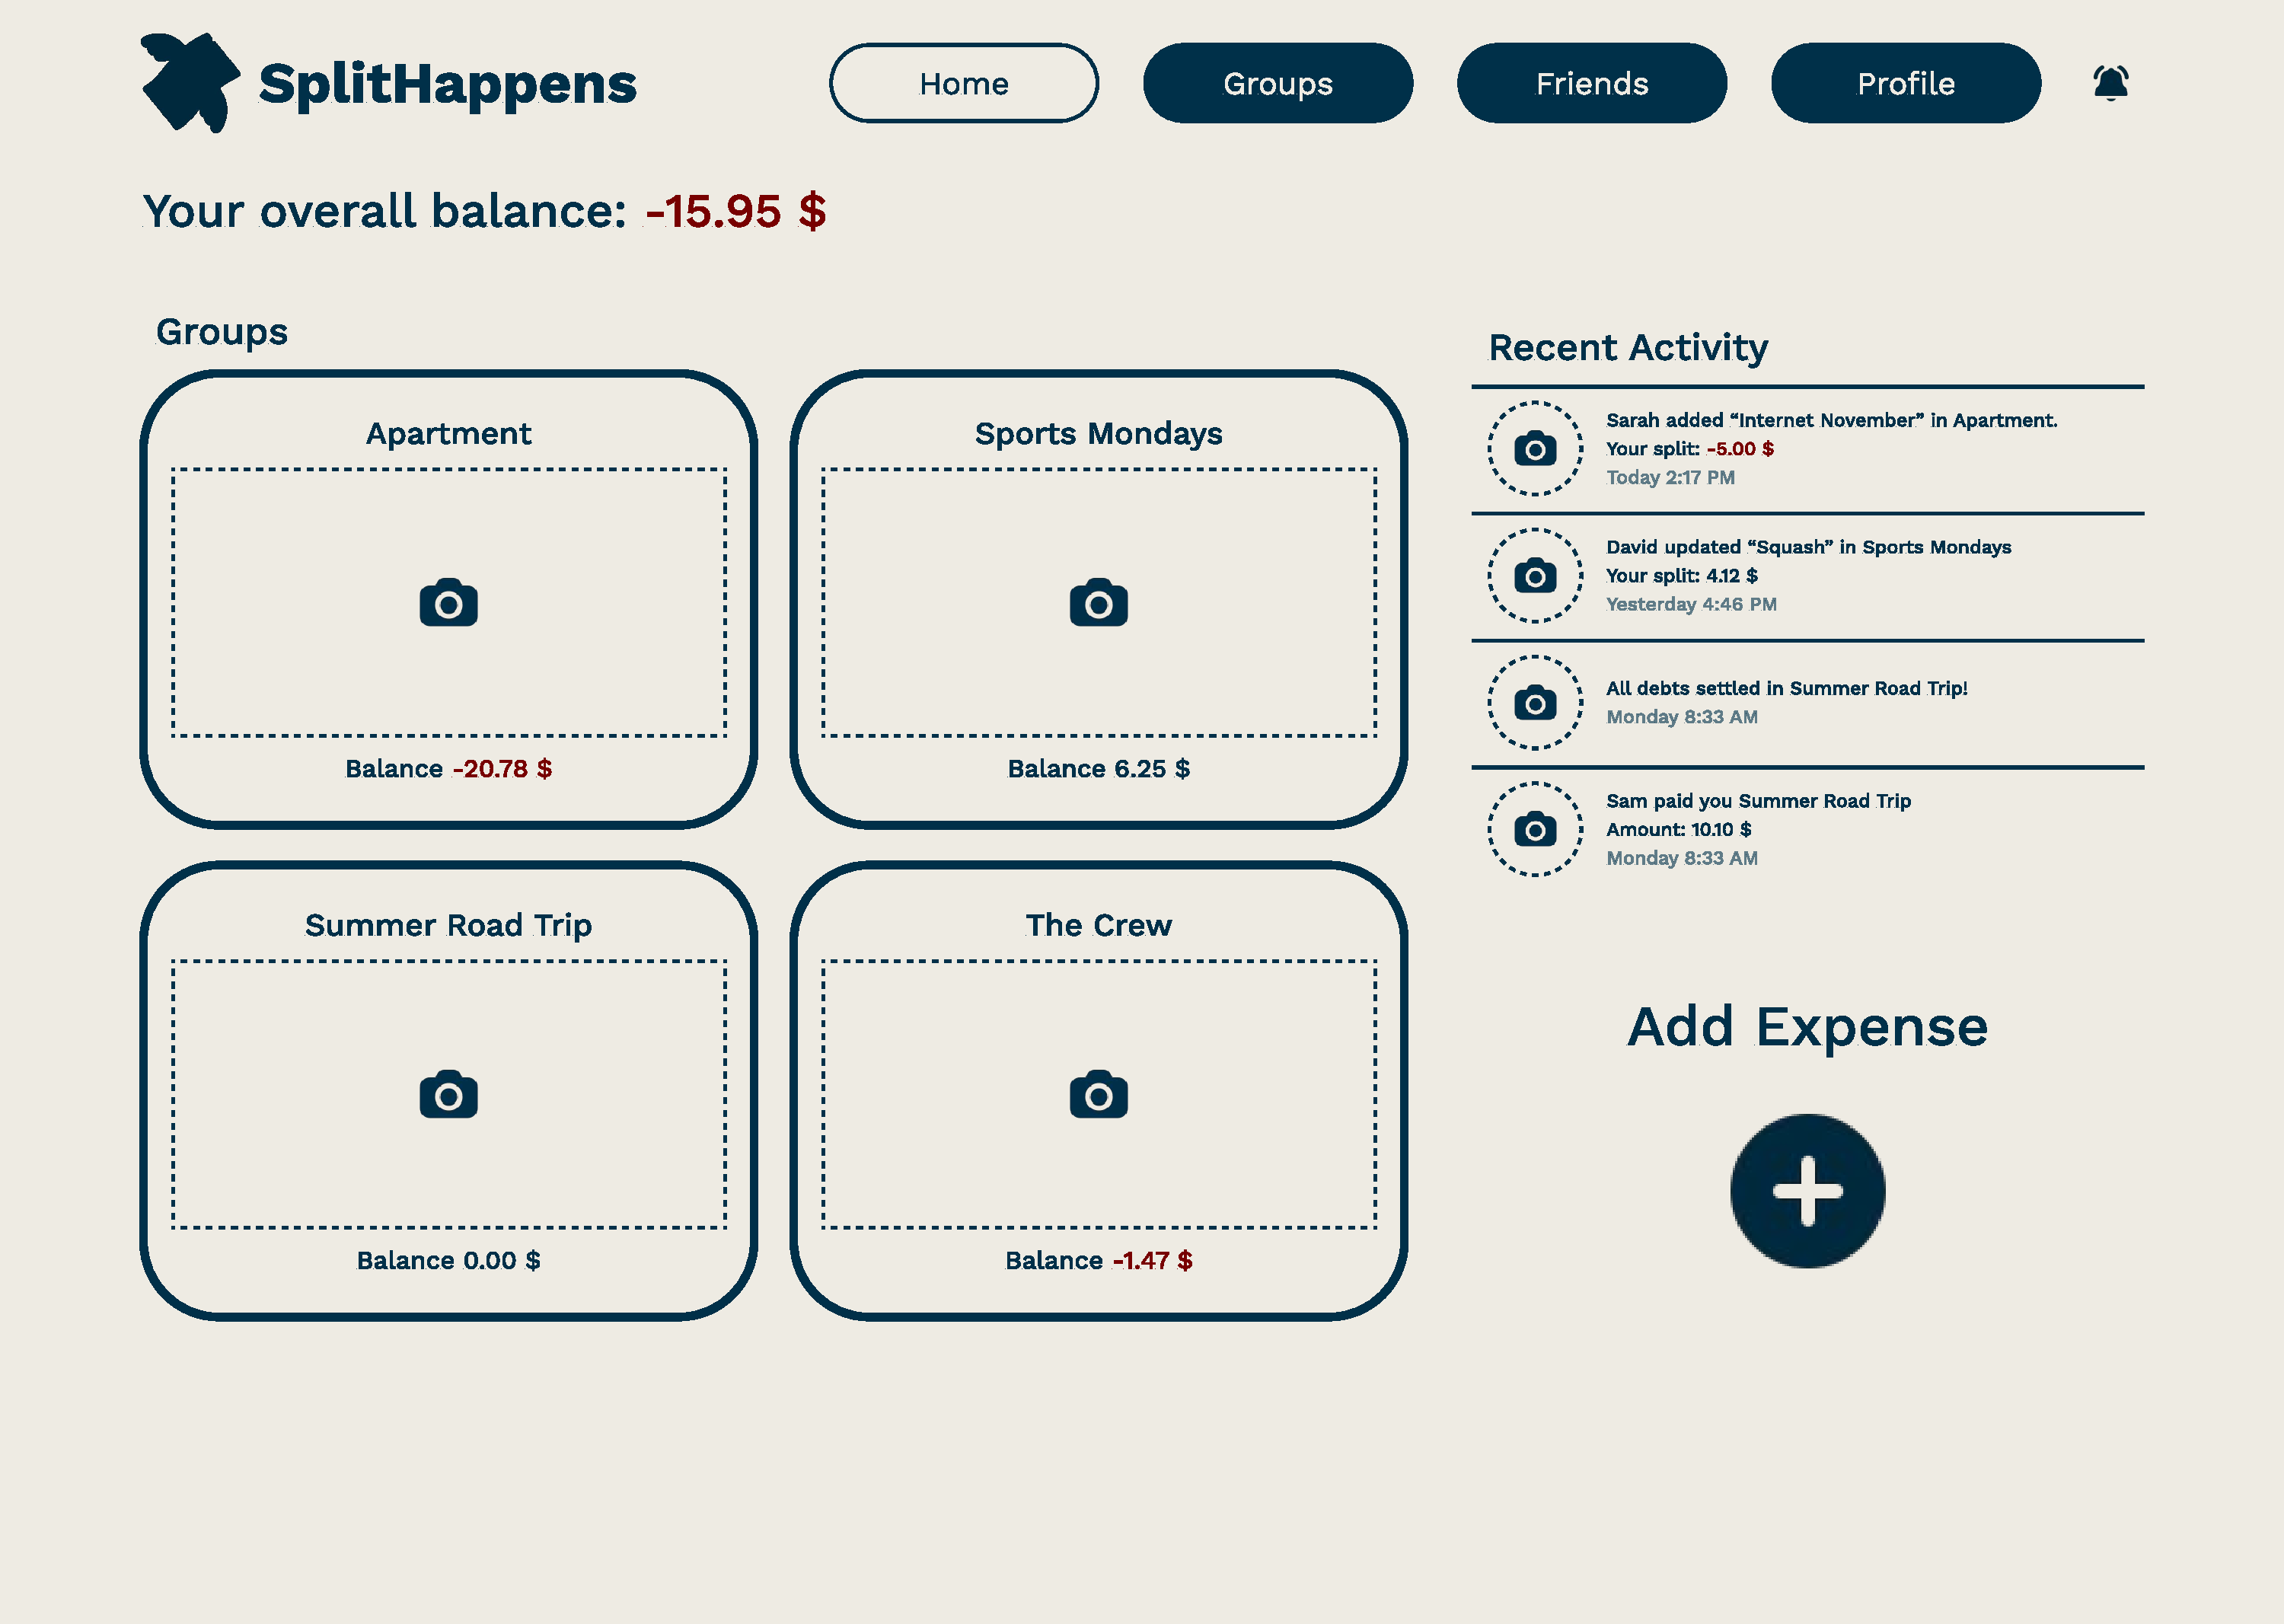
\includegraphics[width=0.9\textwidth]{images/prototype/Homepage.pdf}
    \caption{UI prototype - Desktop home page}
\end{figure}

\begin{figure}[H]
    \centering
    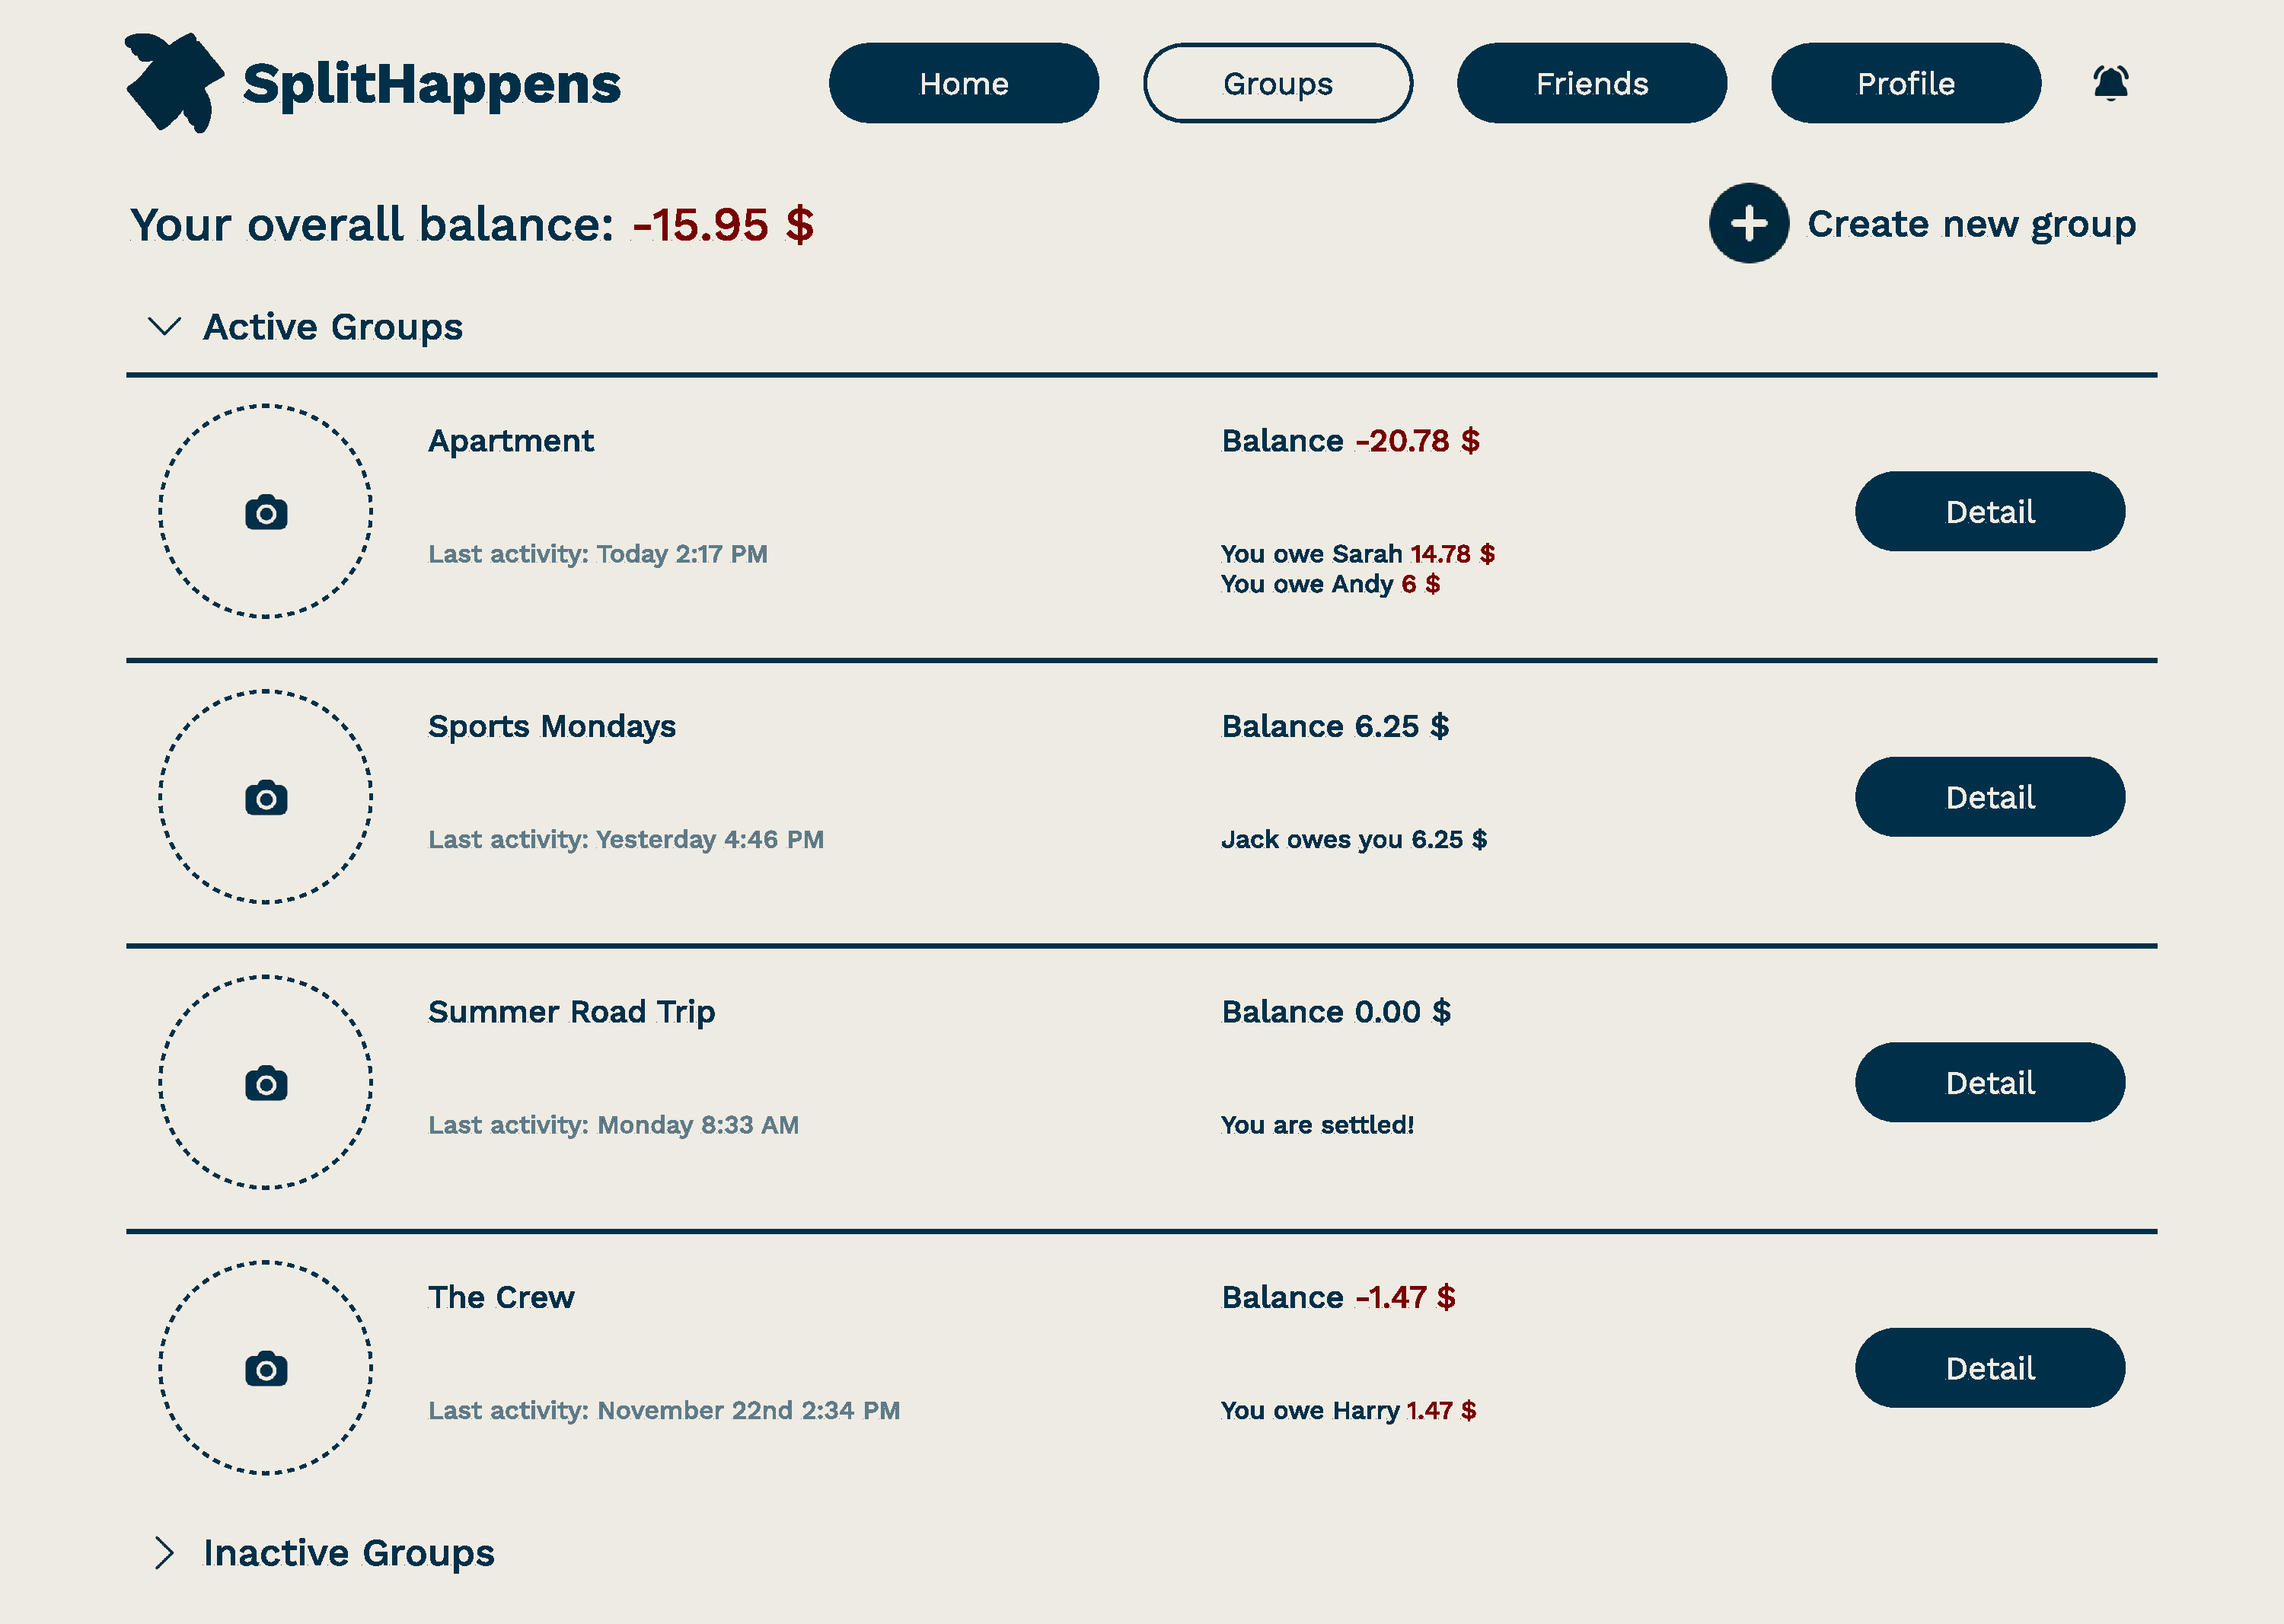
\includegraphics[width=0.9\textwidth]{images/prototype/Groups.pdf}
    \caption{UI prototype - Desktop groups}
\end{figure}

\begin{figure}[H]
    \centering
    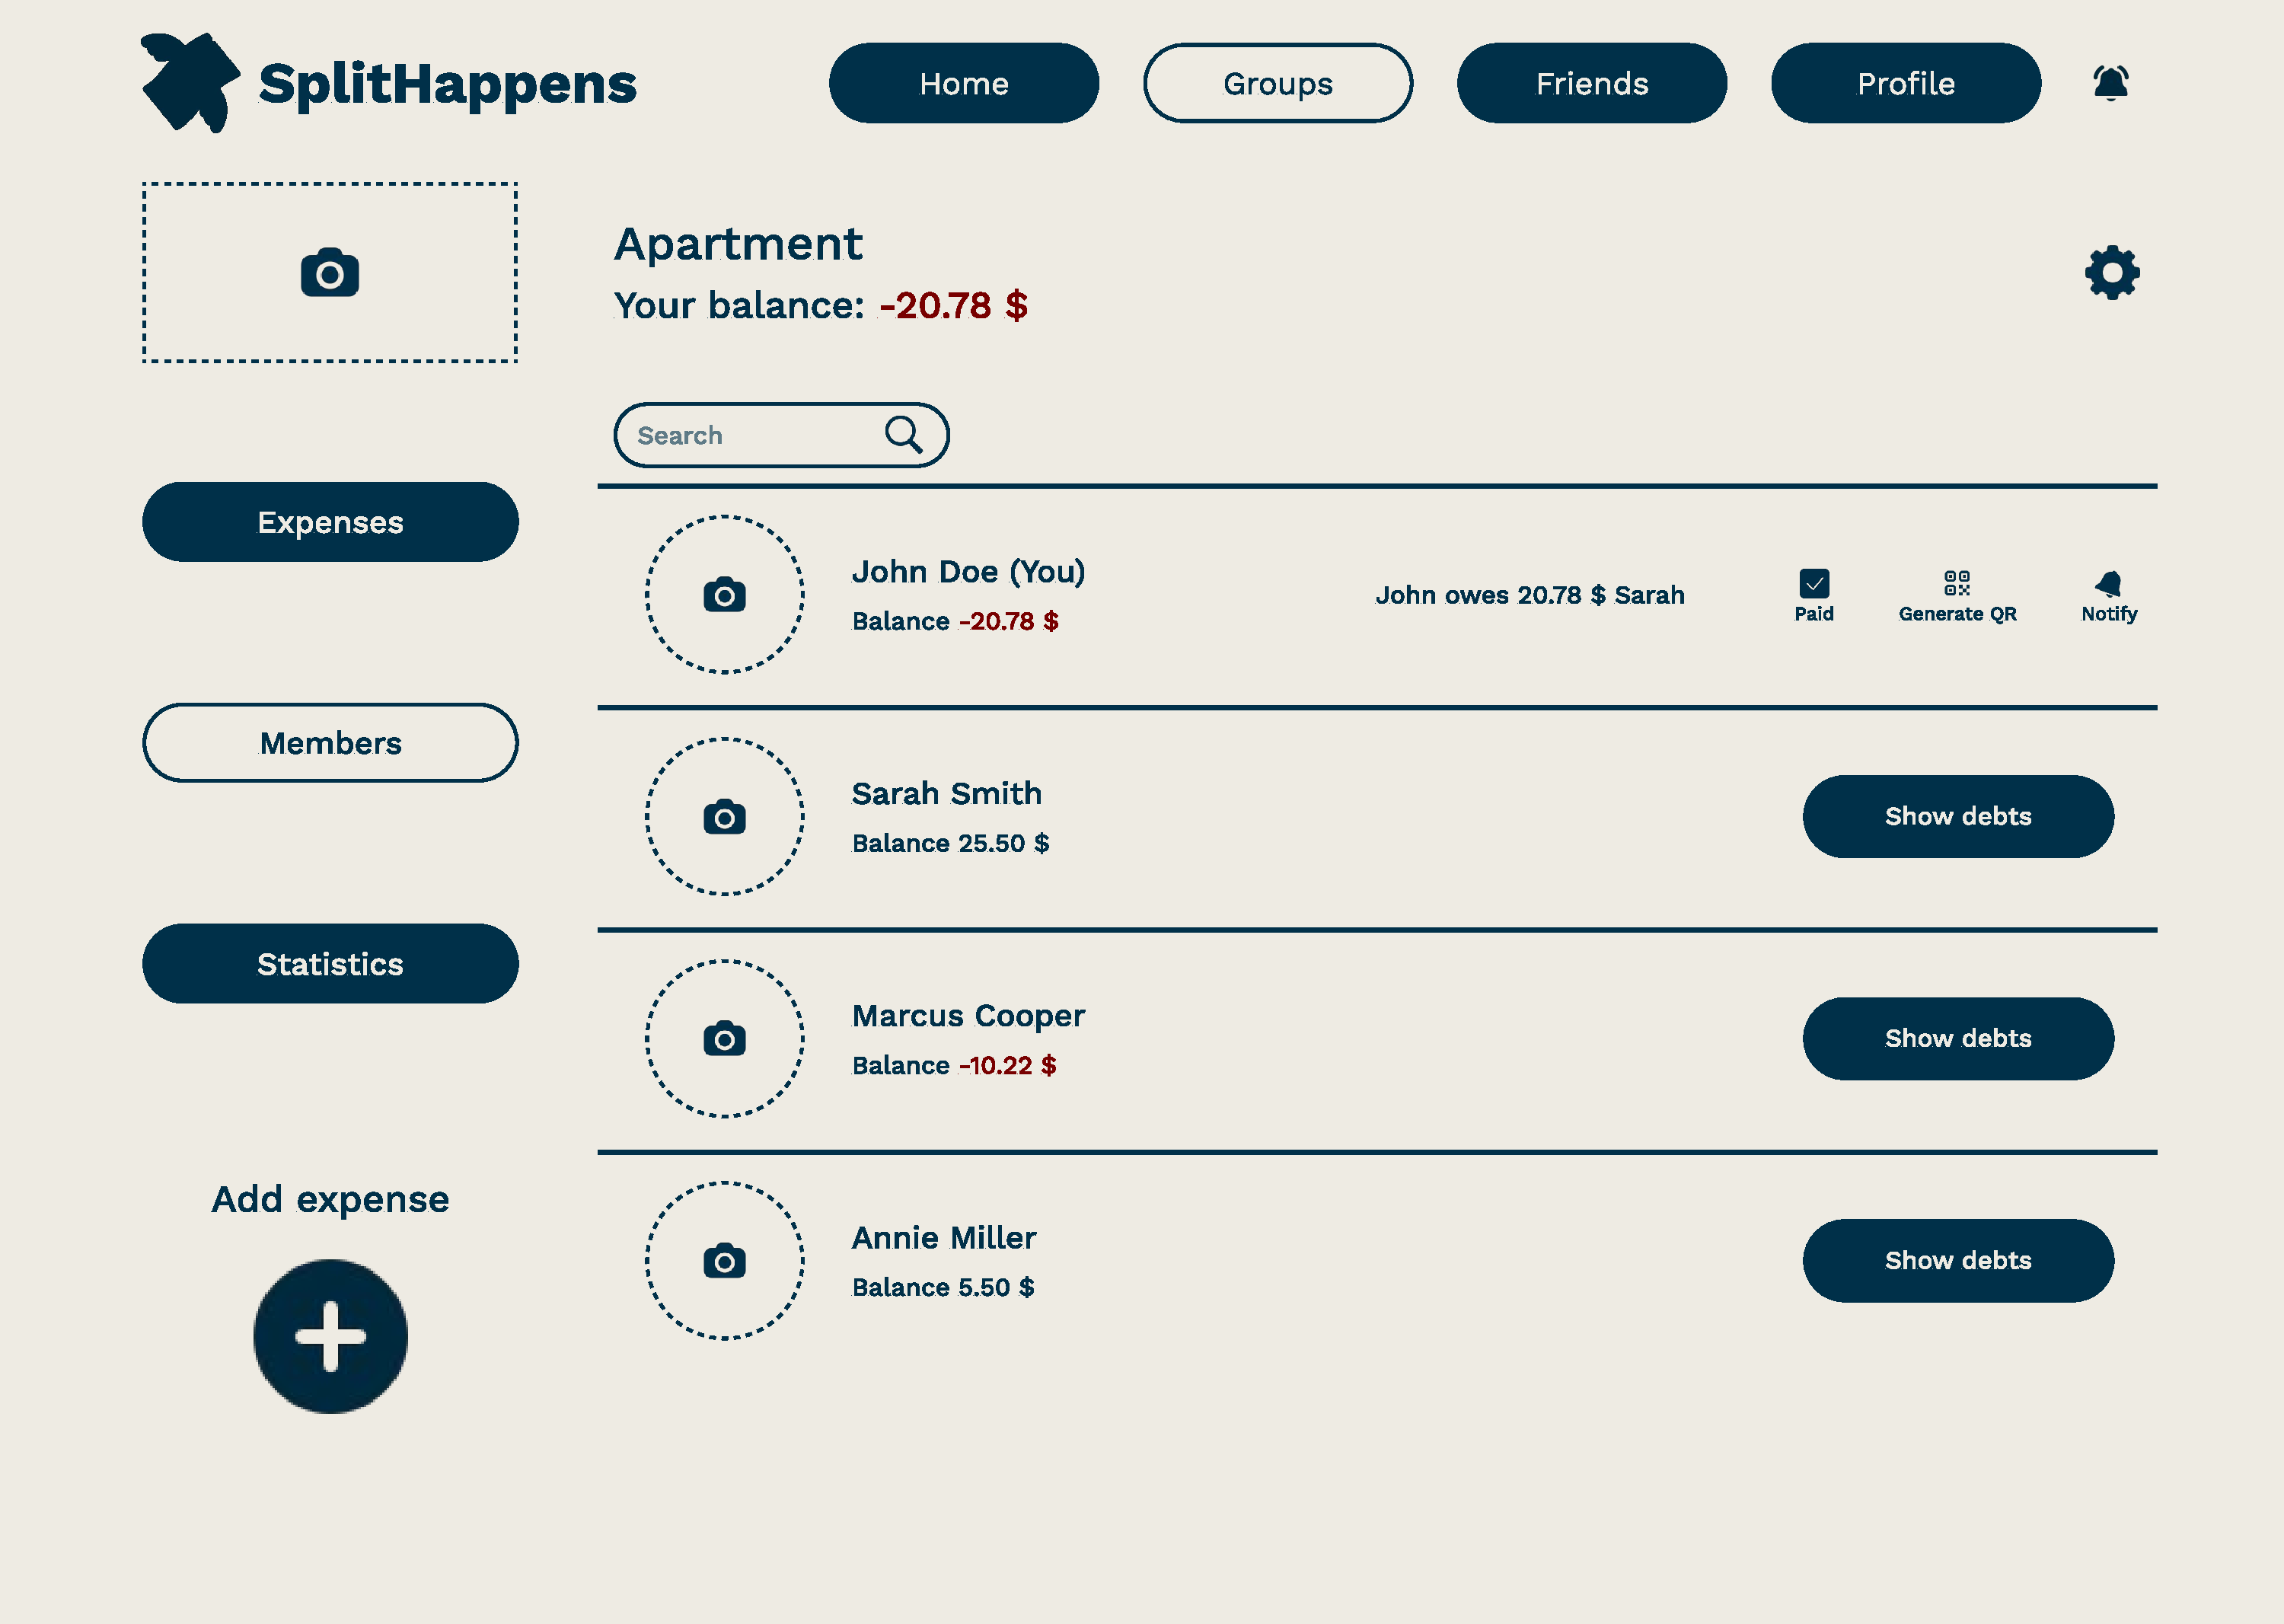
\includegraphics[width=0.9\textwidth]{images/prototype/Group Detail - Members.pdf}
    \caption{UI prototype - Desktop group members}
\end{figure}

\begin{figure}[H]
    \centering
    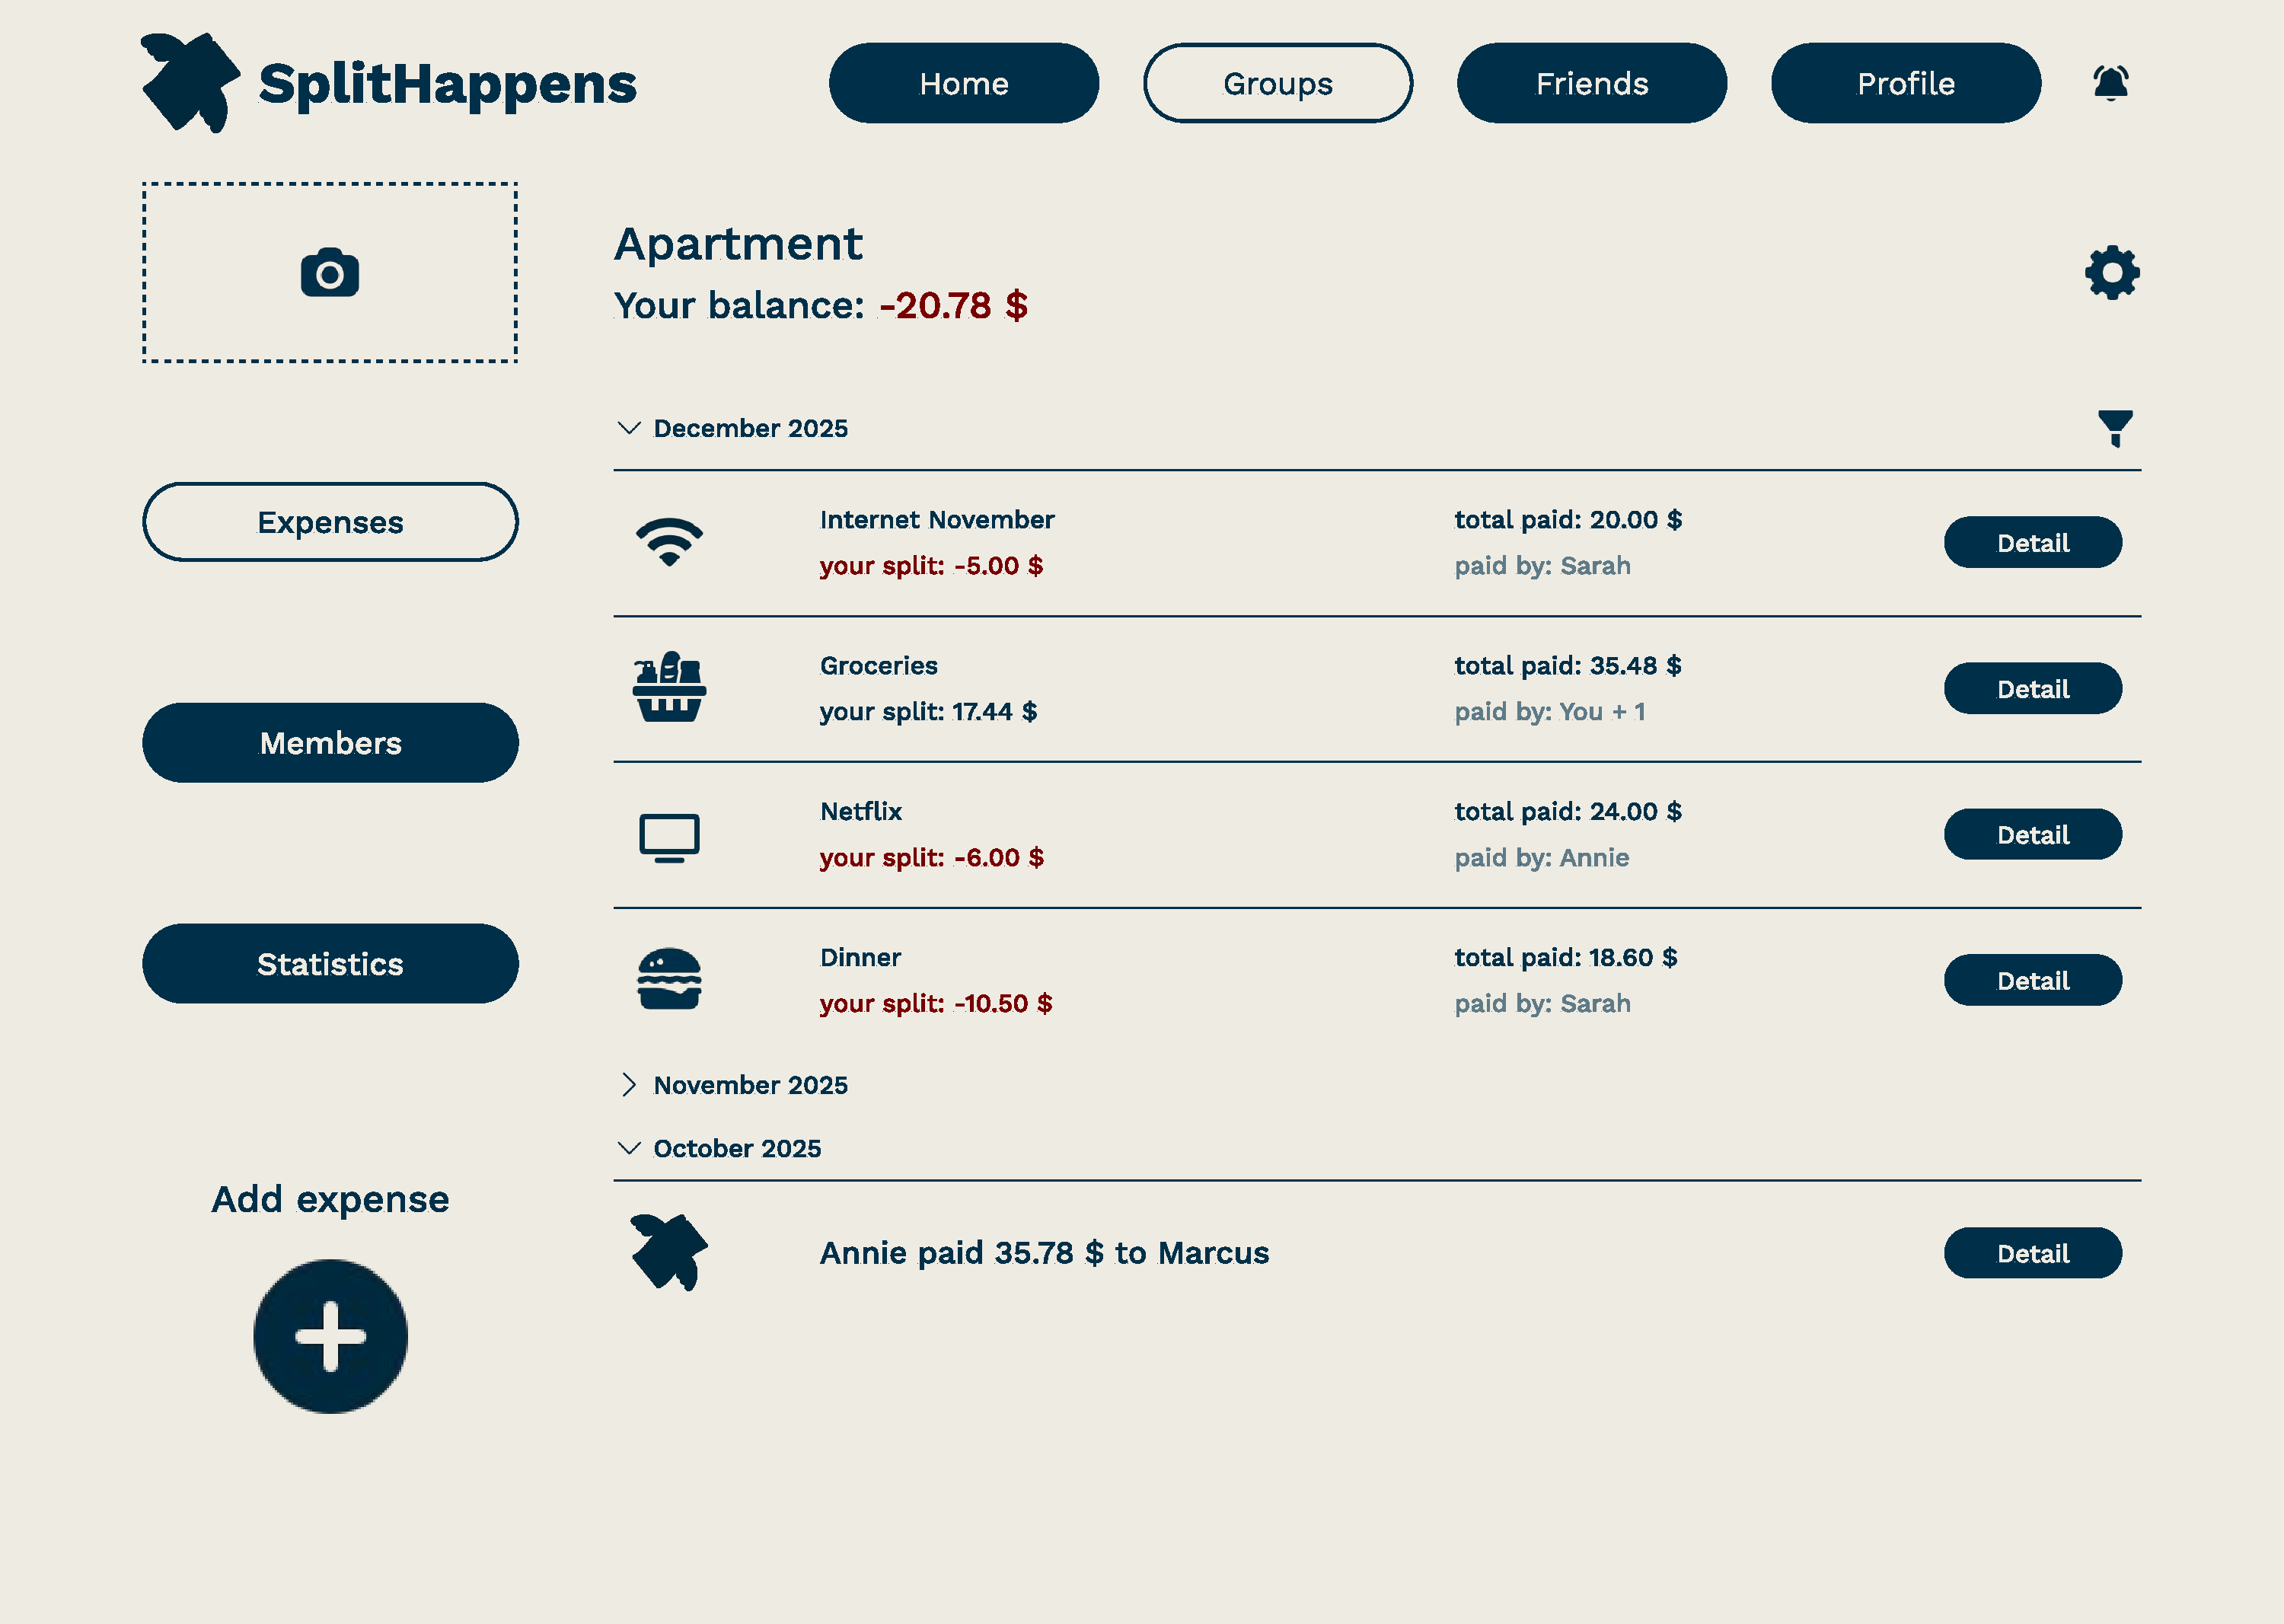
\includegraphics[width=0.9\textwidth]{images/prototype/Group Detail - Expenses.pdf}
    \caption{UI prototype - Desktop expenses in a group}
\end{figure}

\begin{figure}[H]
    \centering
    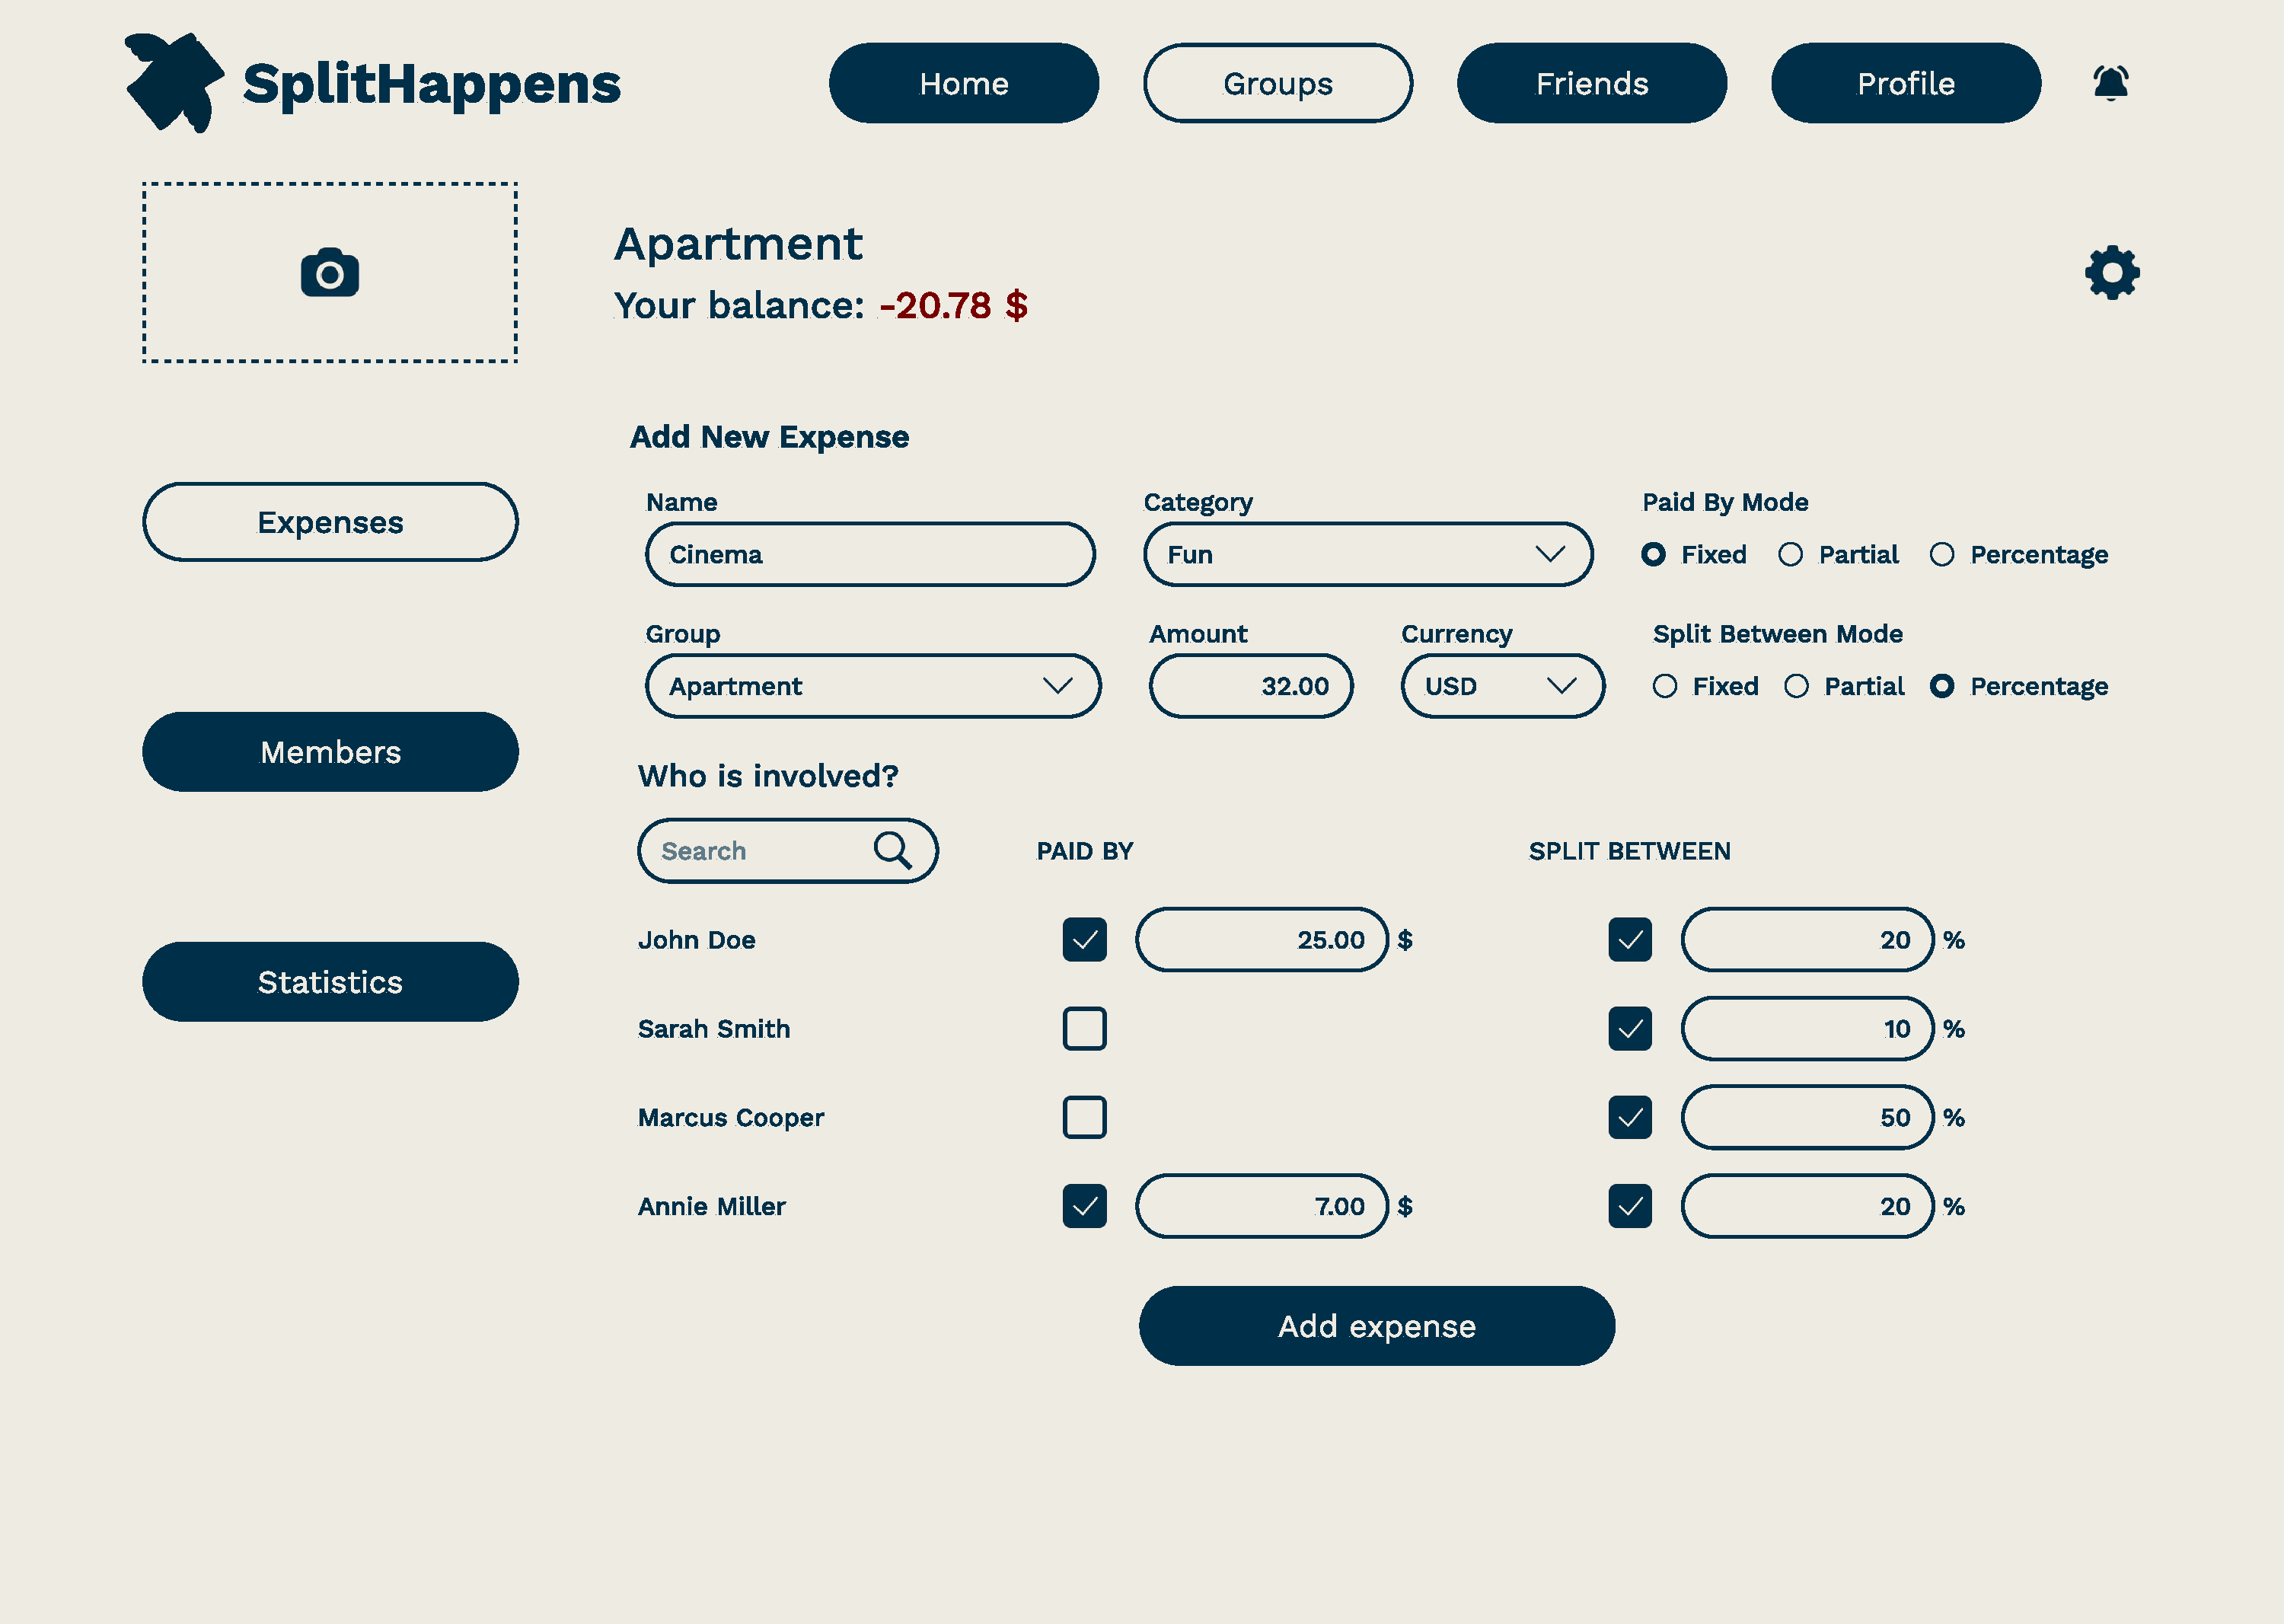
\includegraphics[width=0.9\textwidth]{images/prototype/Group Detail - Add expense.pdf}
    \caption{UI prototype - Desktop add expense interface}
\end{figure}

\section{Mobile screens}

\begin{figure}
    \centering
    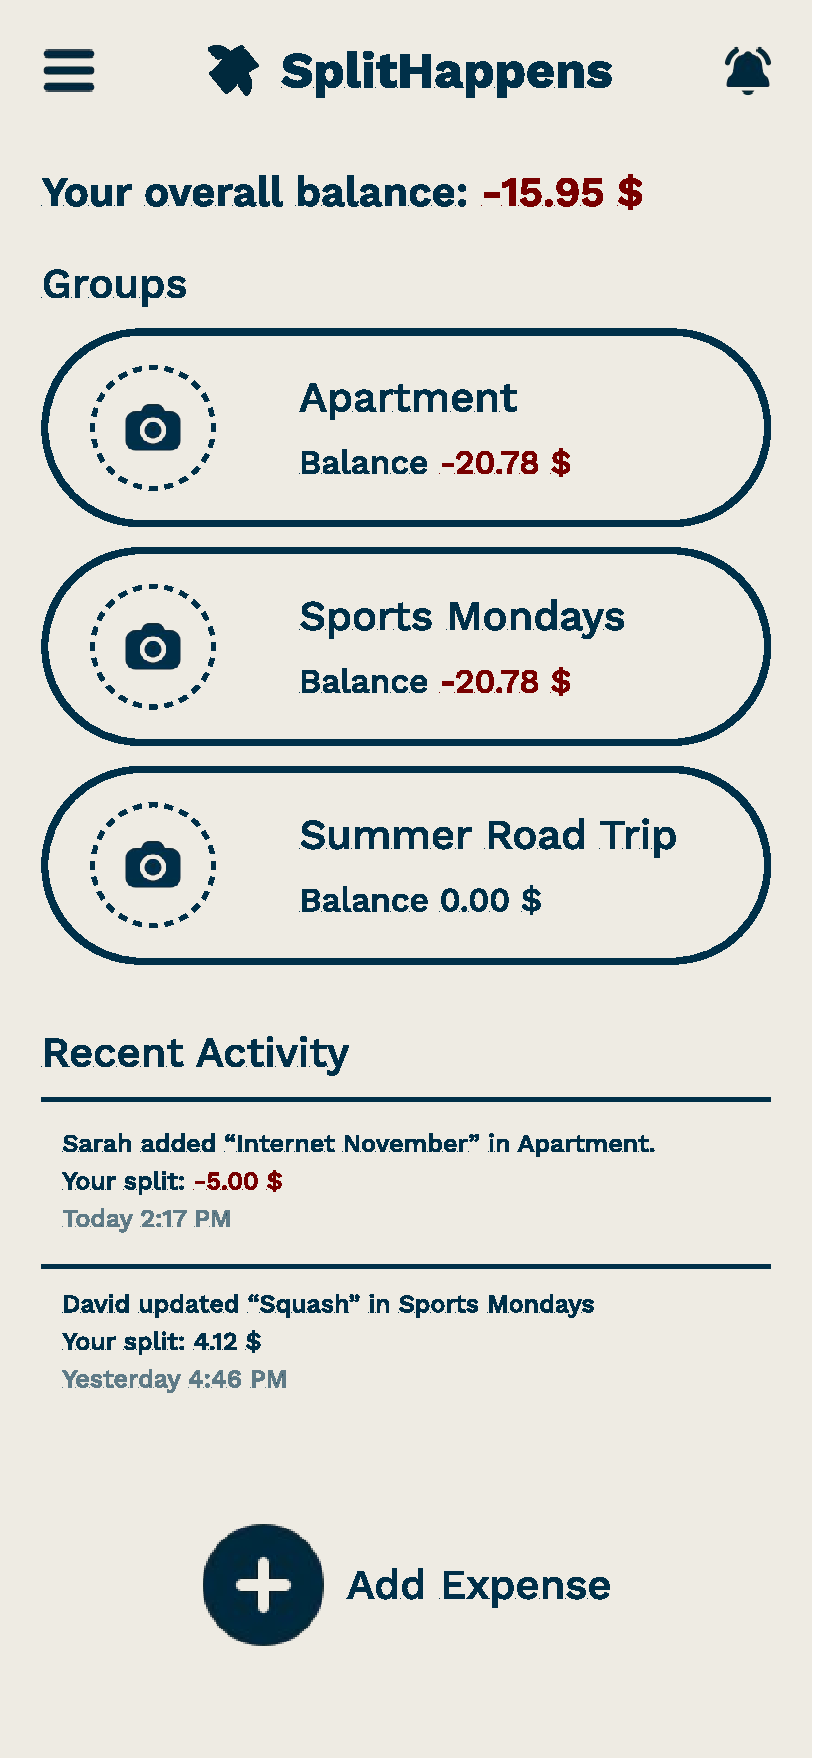
\includegraphics[width=0.3\textwidth]{images/prototype/Mobile Homepage.pdf}
    \hspace{35pt}
    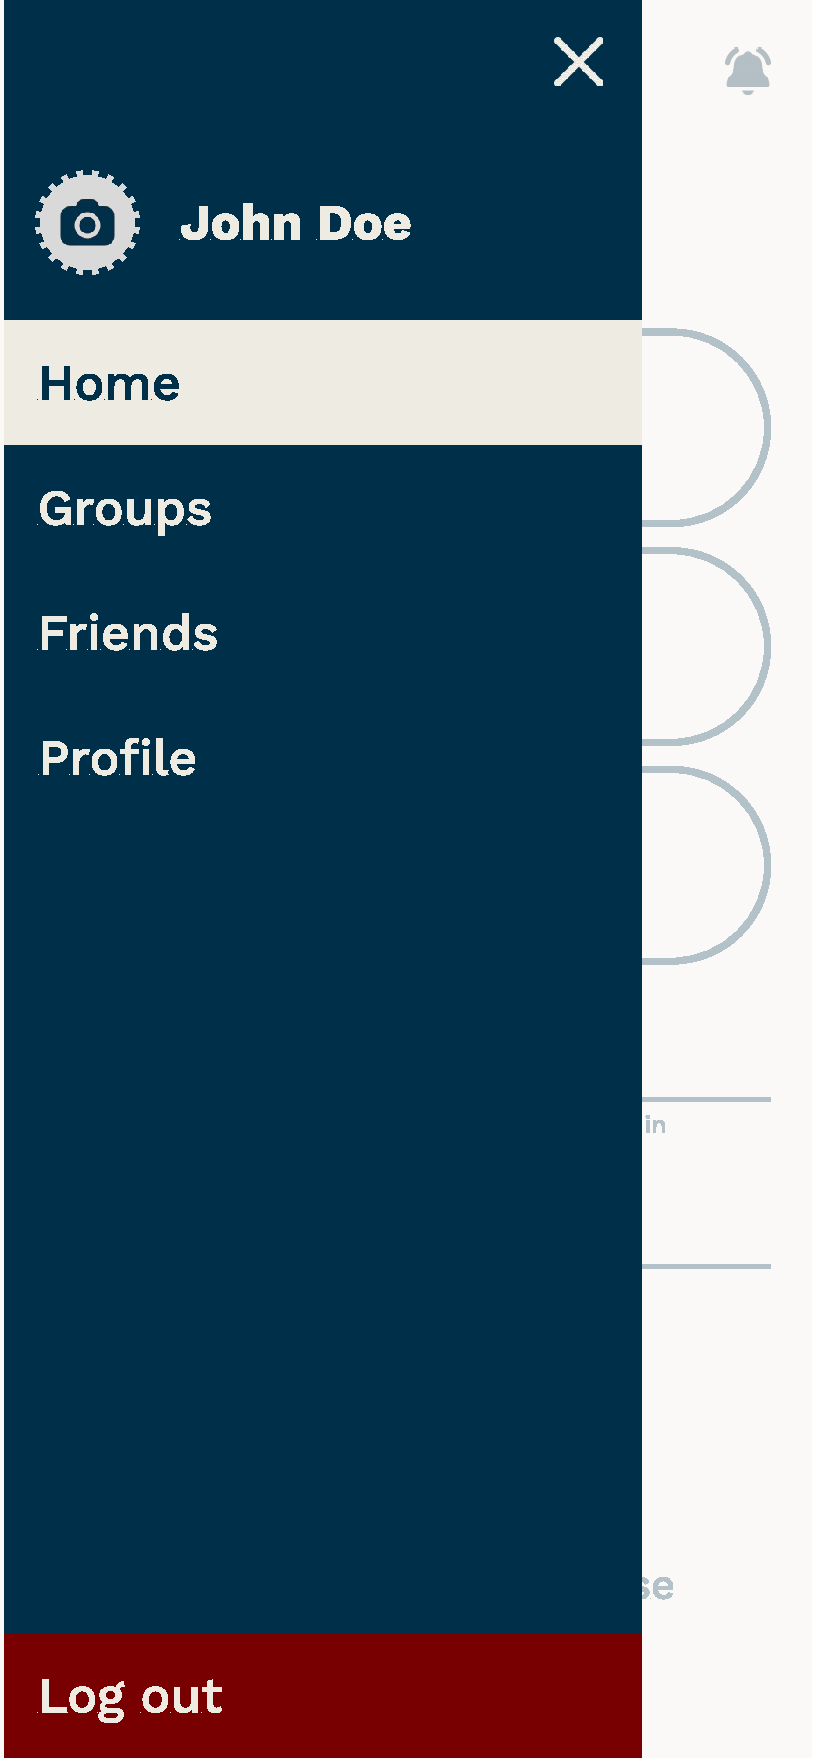
\includegraphics[width=0.3\textwidth]{images/prototype/Mobile Opened Menu.pdf}
    \caption{UI prototype - Mobile homepage and side menu}
\end{figure}

\begin{figure}
    \centering
    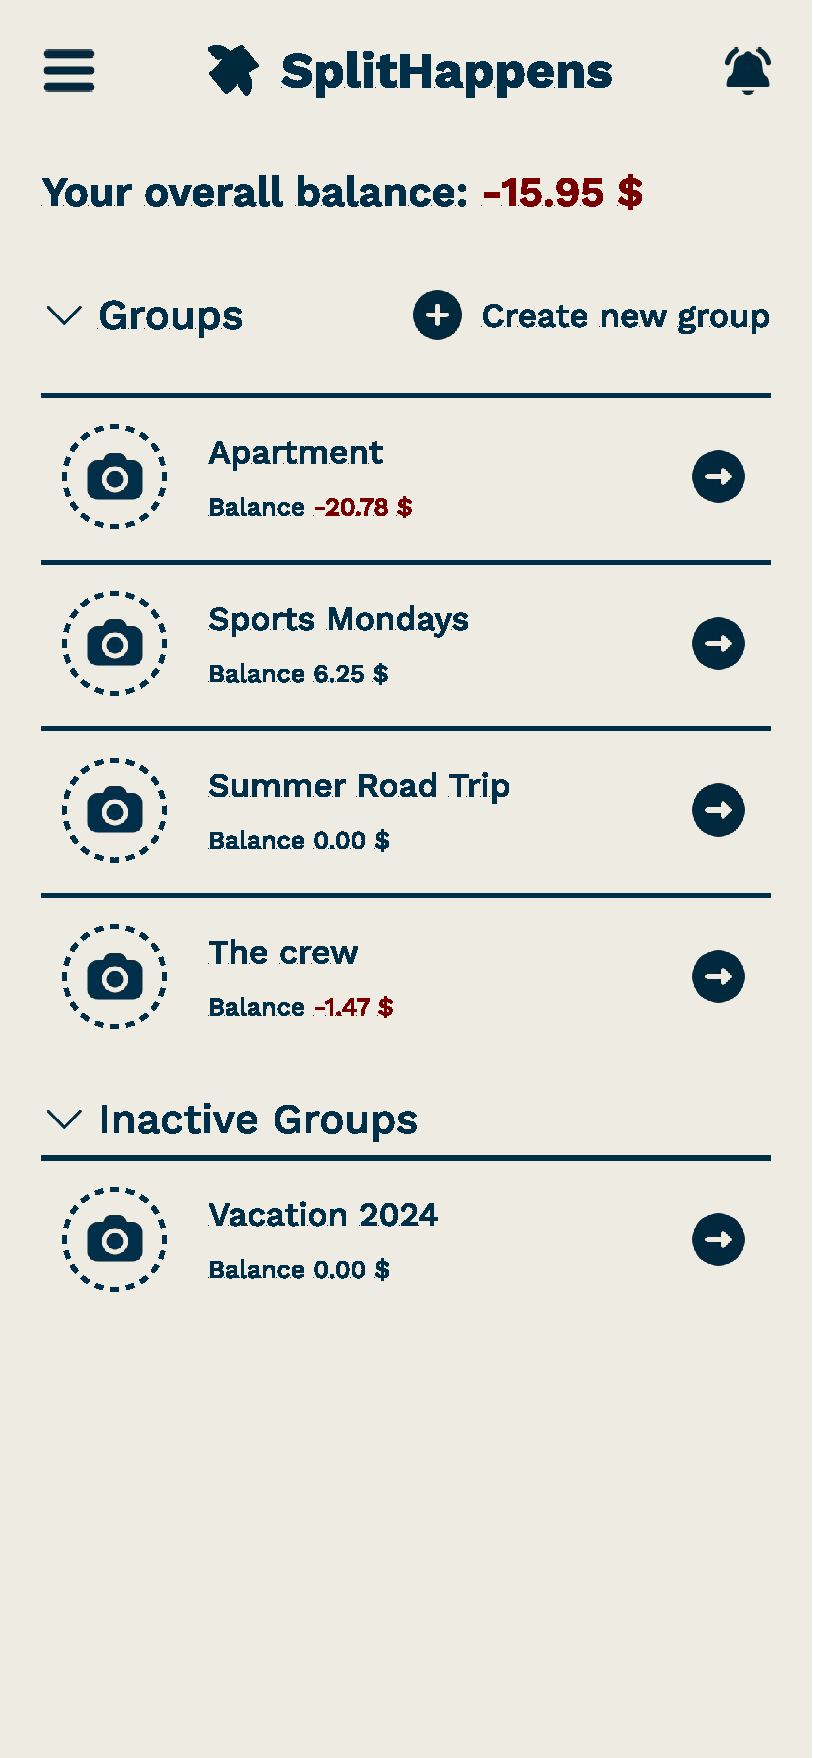
\includegraphics[width=0.3\textwidth]{images/prototype/Mobile Groups.pdf}
    \hspace{35pt}
    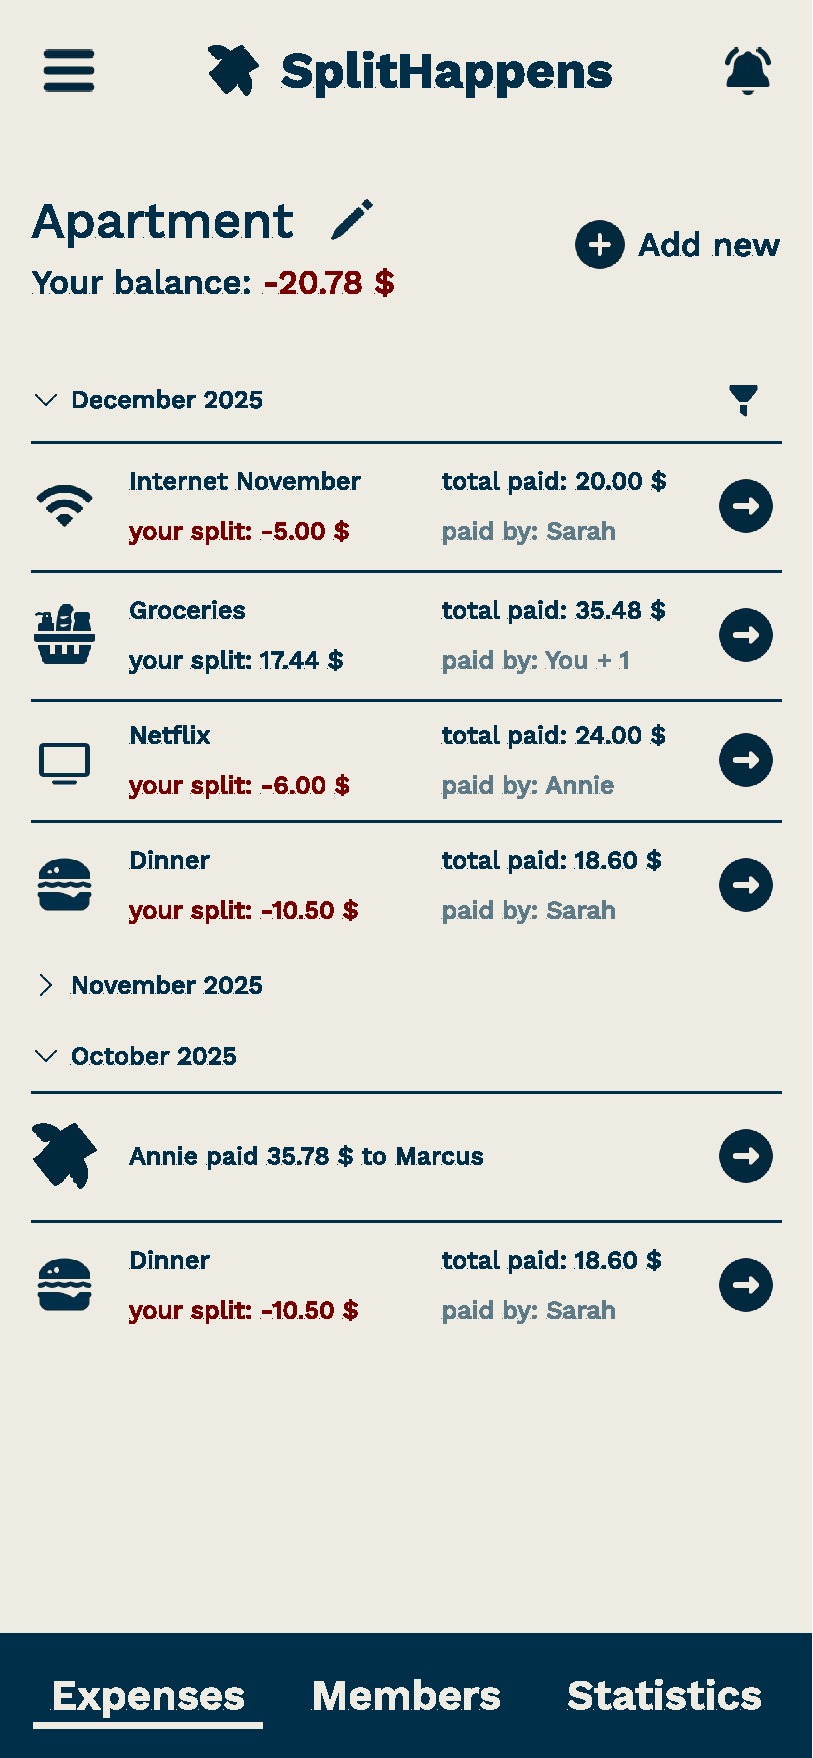
\includegraphics[width=0.3\textwidth]{images/prototype/Mobile Group Detail - Expenses.pdf}
    \caption{UI prototype - Mobile groups and expenses}
\end{figure}

\begin{figure}
    \centering
    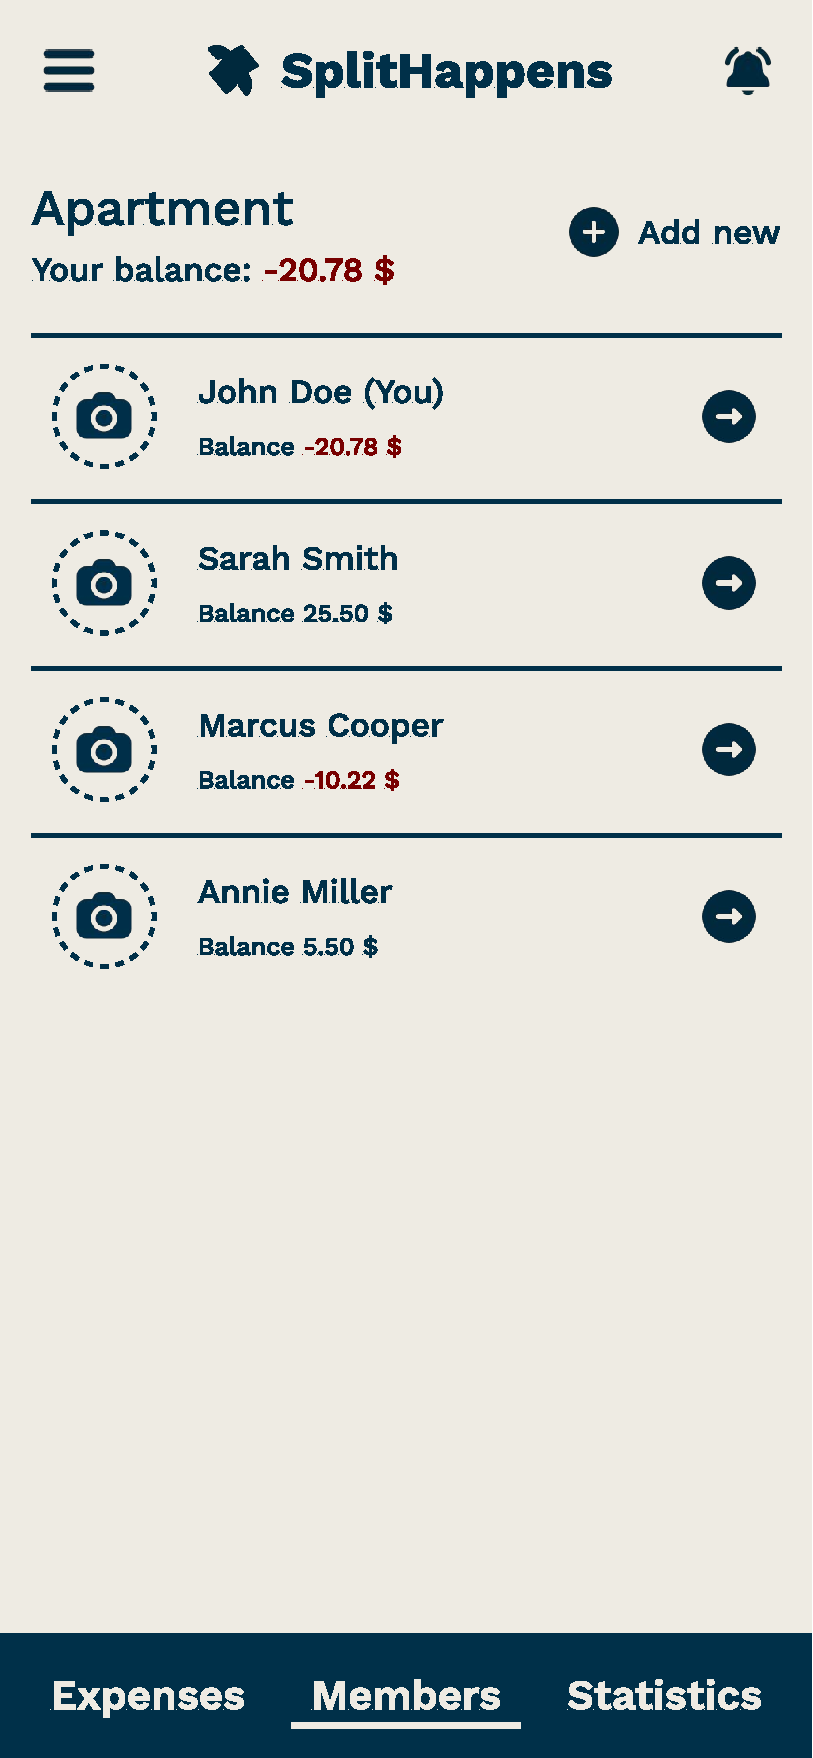
\includegraphics[width=0.3\textwidth]{images/prototype/Mobile Group Detail - Members.pdf}
    \hspace{35pt}
    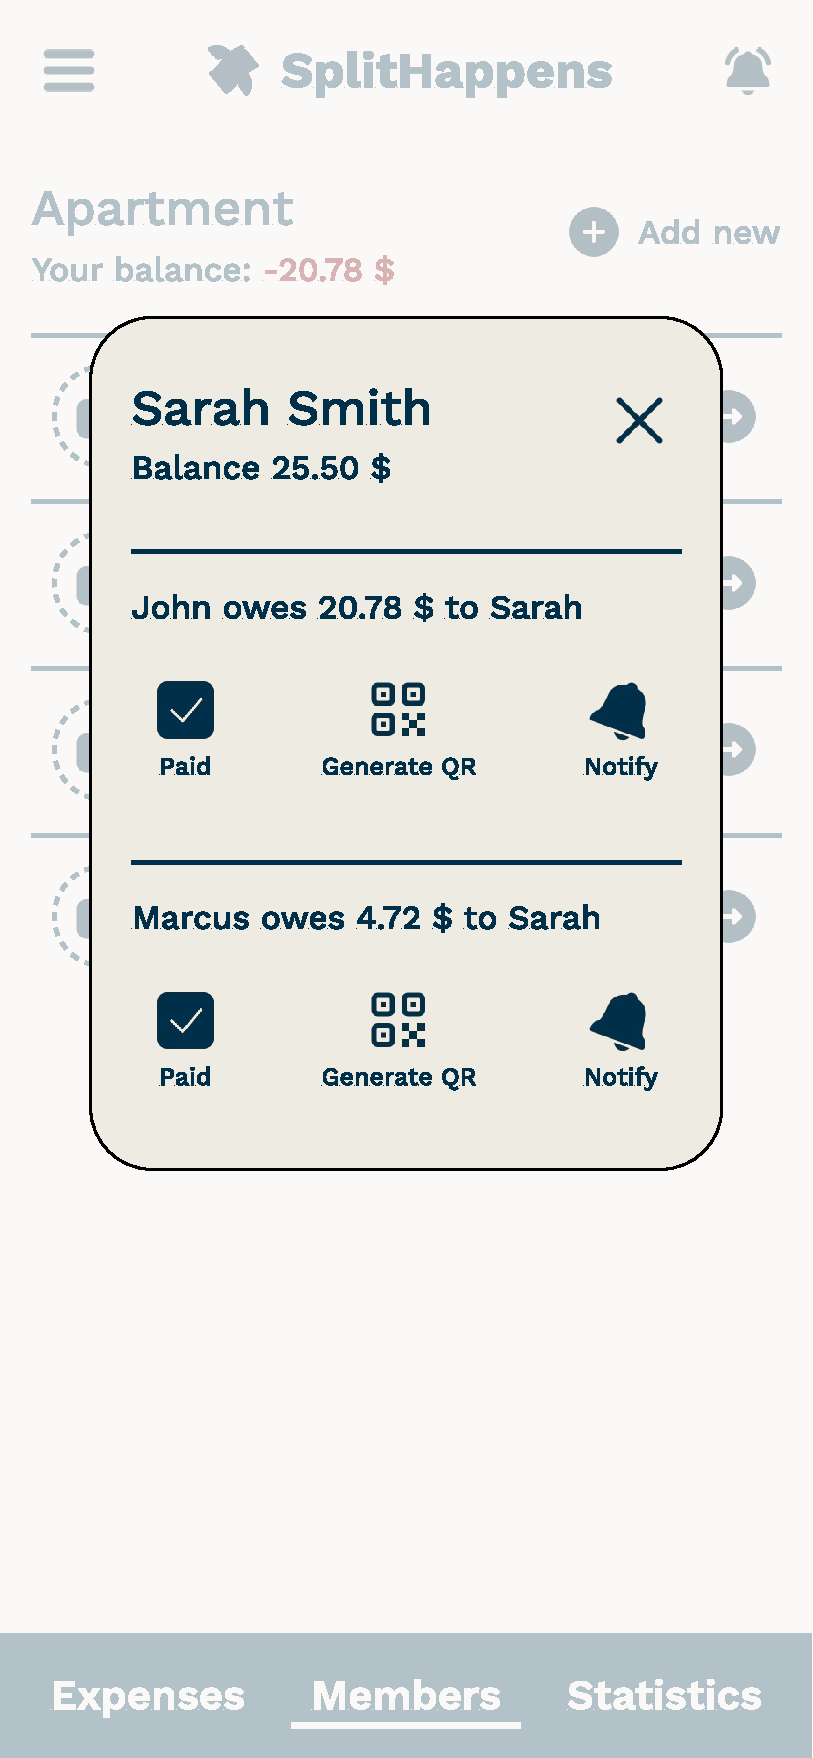
\includegraphics[width=0.3\textwidth]{images/prototype/Mobile Group Detail - Member balances.pdf}
    \caption{UI prototype - Mobile members and member balance detail}
\end{figure}

\begin{figure}
    \centering
    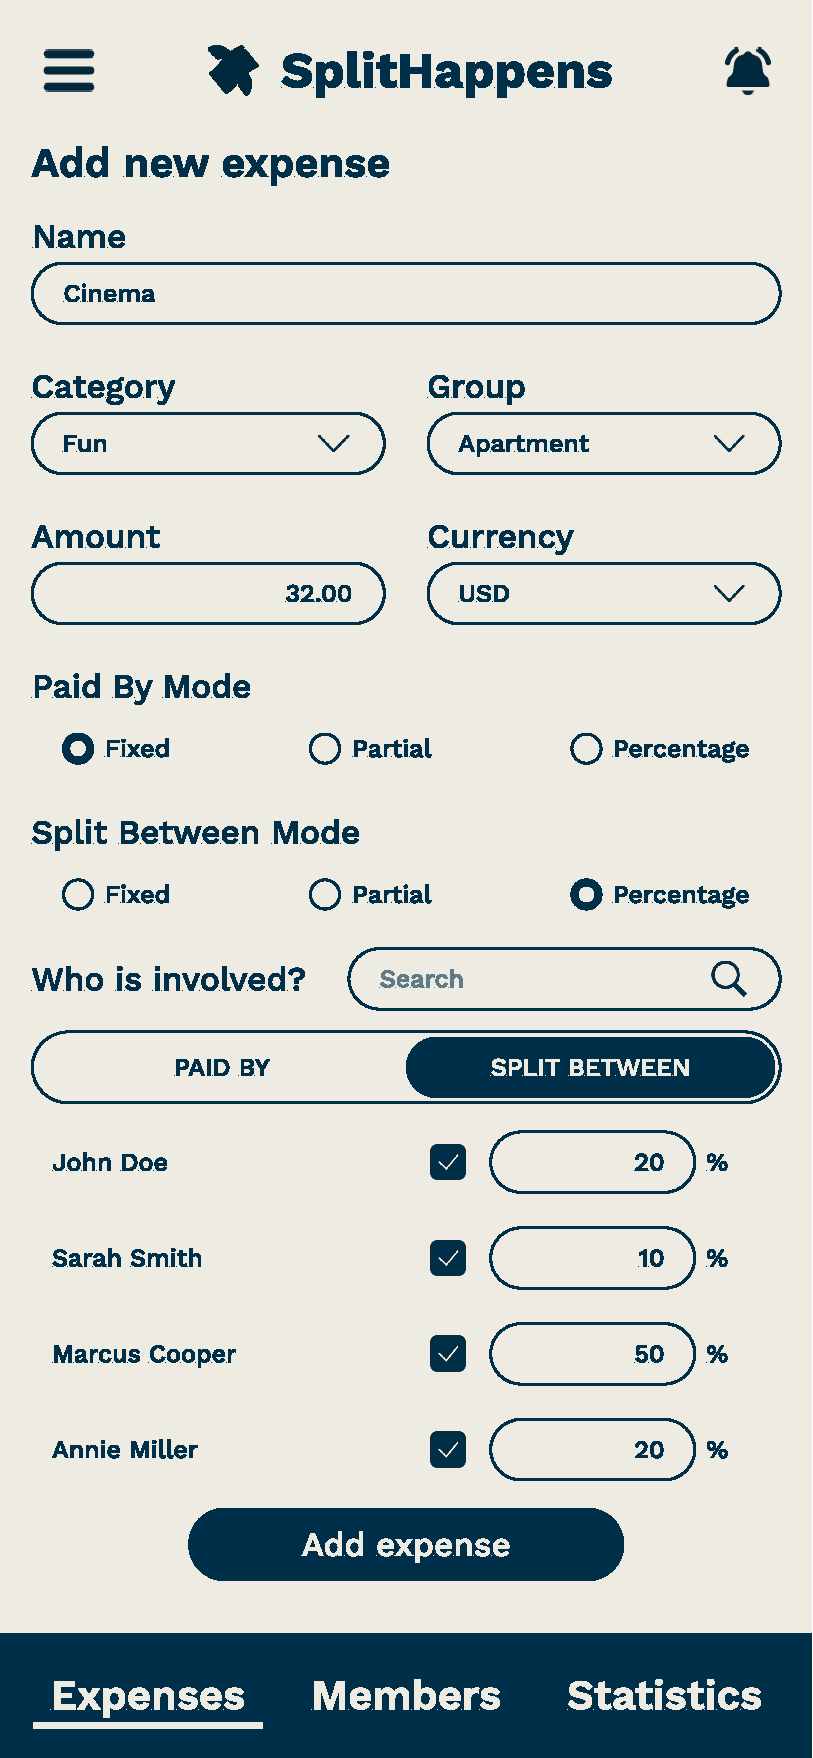
\includegraphics[width=0.3\textwidth]{images/prototype/Mobile Group Detail - Add expense.pdf}
    \caption{UI prototype - Mobile add expense interface}
\end{figure}

\chapter{Test scenarios}
\label{app:b}
\section{Test Scenario 1: User Management}
\textbf{Objective:} To verify that the system correctly handles the full lifecycle of a user account, from creation and authentication to profile customization.

\begin{enumerate}
    \item Sign up
    \item Login
    \item Edit your profile information
    \item Upload profile picture
\end{enumerate}

\section{Test Scenario 2: Group Management}
\textbf{Objective:} To verify that the system correctly handles the full lifecycle of a group, from initial creation and group customization and member management.

\begin{enumerate}
    \item Create new group
    \item Edit group information
    \item Add new members
    \item Upload group picture
\end{enumerate}

\section{Test Scenario 3: Expenses and Payments}
\textbf{Objective:} To verify that the system correctly handles the full lifecycle of expenses, like various split modes and the final simplification of debts to reduce the number of transactions.

\begin{enumerate}
    \item Add three different expenses (any group)
    \item Edit one of the expenses
    \item Record a payment
    \item Generate a QR code payment
\end{enumerate}

\section{Test Scenario 4: Friends}
\textbf{Objective:} To verify that the system correctly handles the full lifecycle of a friend relationship, like request handling, or non-group expenses.

\begin{enumerate}
    \item Add a friend
    \item Add a non-group expense with that friend
    \item Settle with a friend
    \item Remove a friend
\end{enumerate}

\section{Test Scenario 5: Statistics \& Notifications}
\textbf{Objective:} To verify that the system shows all needed statistics and that they are intuitive and clear to the user. For notifications, verify that notifications are clear and shown properly.

\begin{enumerate}
    \item Add three different expenses in a group (can be any group)
    \item Review statistics
    \item Review fired notifications
    \item Mark notifications as read
\end{enumerate}

\end{document}